% !TeX program = pdflatex

\documentclass{thesis}

\usepackage{lipsum} % Dummy text for examples
\usepackage{graphicx}
\usepackage{xspace}
\usepackage[space]{grffile}
\usepackage{latexsym}
\usepackage{textcomp}
\usepackage{longtable}
\usepackage{multirow,booktabs}
\usepackage{amsfonts,amsmath,amssymb}
\usepackage{natbib}
\usepackage{url}
\usepackage[utf8]{inputenc}
\usepackage[english]{babel}
\usepackage[hidelinks,pagebackref]{hyperref} % Handy for links, can comment for plain PDF
%%%%%%%%%%%%%%%%%%%%%%%
%%% Commands
%%%%%%%%%%%%%%%%%%%%%%%
%Units
\newcommand{\kelvin}{\ensuremath{\,\mathrm{K}}\xspace}
\newcommand{\s}{\ensuremath{\,\mathrm{s}}\xspace}
\newcommand{\grams}{\ensuremath{\,\mathrm{g}}\xspace}
\newcommand{\cm}{\ensuremath{\,\mathrm{cm}}\xspace}
\newcommand{\cc}{\ensuremath{\,\mathrm{cm}^{-3}}\xspace}
\newcommand{\msun}{\ensuremath{\,\mathrm{M}_{\odot}}\xspace}
\newcommand{\rsun}{\ensuremath{\,\mathrm{R}_{\odot}}\xspace}
\newcommand{\zsun}{\ensuremath{\,\mathrm{Z}_{\odot}}\xspace}
\newcommand{\kms}{\ensuremath{\,\mathrm{km}\,\mathrm{s}^{-1}\xspace}}
\newcommand{\kpc}{\ensuremath{\,\mathrm{kpc}}\xspace}
\newcommand{\pc}{\ensuremath{\,\mathrm{pc}}\xspace}
\newcommand{\au}{\ensuremath{\,\mathrm{AU}}\xspace}
\newcommand{\Mpc}{\ensuremath{\,\mathrm{Mpc}}\xspace}
\newcommand{\yrs}{\ensuremath{\,\mathrm{yrs}}\xspace}
\newcommand{\yr}{\ensuremath{\,\mathrm{yr}}\xspace}
\newcommand{\myr}{\ensuremath{\,\mathrm{Myr}}\xspace}
\newcommand{\ev}{\ensuremath{\,\mathrm{eV}}\xspace}
\newcommand{\kev}{\ensuremath{\,\mathrm{keV}}\xspace}
\newcommand{\erg}{\ensuremath{\,\mathrm{erg}}\xspace}
\newcommand{\sr}{\ensuremath{\,\mathrm{sr}}\xspace}
\newcommand{\Hz}{\ensuremath{\,\mathrm{Hz}}\xspace}
%Constants
\newcommand{\kb}{k_{\mathrm{B}}}
\newcommand{\mh}{m_{\mathrm{H}}}
%Special values
\newcommand{\tcmb}{\ensuremath{{T}_{\mathrm{CMB}}}\xspace}
\newcommand{\tff}{\ensuremath{{t}_{\mathrm{ff}}}\xspace}
\newcommand{\tH}{\ensuremath{{t}_{\textsc{h}}}\xspace}
\newcommand{\zcrit}{\ensuremath{{Z}_{\mathrm{crit}}}\xspace}
\newcommand{\ncrit}{\ensuremath{{n}_\mathrm{crit}}\xspace}
\newcommand{\tvir}{\ensuremath{{T}_{\mathrm{vir}}}\xspace}
\newcommand{\rvir}{\ensuremath{{R}_{\mathrm{vir}}}\xspace}
\newcommand{\mvir}{\ensuremath{{M}_{\mathrm{vir}}}\xspace}
\newcommand{\rta}{\ensuremath{{R}_{\mathrm{ta}}}\xspace}
%Chemistry
\newcommand{\htwo}{\ensuremath{\mathrm{H}_2}\xspace}
\newcommand{\hd}{\ensuremath{\mathrm{HD}}\xspace}
\newcommand{\deut}{\ensuremath{\mathrm{D}}\xspace}
\newcommand{\h}{\ensuremath{\mathrm{H}}\xspace}
\newcommand{\hplus}{\ensuremath{\mathrm{H}^+}\xspace}
\newcommand{\hminus}{\ensuremath{\mathrm{H}^-}\xspace}
\newcommand{\he}{\ensuremath{\mathrm{He}}\xspace}
\newcommand{\heplus}{\ensuremath{\mathrm{He}^+}\xspace}
\newcommand{\heminus}{\ensuremath{\mathrm{He}^-}\xspace}
\newcommand{\HI}{\ensuremath{\mathrm{H\,\textsc{i}}}\xspace}
\newcommand{\HeI}{\ensuremath{\mathrm{He\,\textsc{i}}}\xspace}
\newcommand{\HeII}{\ensuremath{\mathrm{He\,\textsc{ii}}}\xspace}
\newcommand{\abunde}{\ensuremath{ x_{\mathrm{e}}}\xspace}
\newcommand{\abundhe}{\ensuremath{ x_{\mathrm{He}}}\xspace}
\newcommand{\abundd}{\ensuremath{ x_{\mathrm{D}}}\xspace}
\newcommand{\abundhd}{\ensuremath{ x_{\mathrm{HD}}}\xspace}
\newcommand{\abundhtwo}{\ensuremath{ x_{\mathrm{H}_2} }\xspace}
\newcommand{\abundhplus}{\ensuremath{ x_{\mathrm{H}^+}}\xspace}
\newcommand{\abundi}{\ensuremath{ x_i}\xspace}
%Energetics
\newcommand{\etot}{\ensuremath{{E}_{\mathrm{tot}}}\xspace}
\newcommand{\egrav}{\ensuremath{{E}_{\mathrm{grav}}}\xspace}
\newcommand{\etherm}{\ensuremath{{E}_{\mathrm{th}}}\xspace}
\newcommand{\ekin}{\ensuremath{{E}_{\mathrm{kin}}}\xspace}
\newcommand{\erot}{\ensuremath{{E}_{\mathrm{rot}}}\xspace}
\newcommand{\ucr}{\ensuremath{{u}_{\textsc{cr}}}\xspace}
\newcommand{\ucrz}{\ensuremath{{u}_{\textsc{cr}}(z)}\xspace}
\newcommand{\uxr}{\ensuremath{{u}_{\textsc{xr}}}\xspace}
\newcommand{\uxrz}{\ensuremath{{u}_{\textsc{xr}}(z)}\xspace}
\newcommand{\gxr}{\ensuremath{\Gamma_{\textsc{xr}}}\xspace}
\newcommand{\gcrit}{\ensuremath{\Gamma_{\textsc{xr}, \mathrm{crit}}}\xspace}
\newcommand{\gblowout}{\ensuremath{\Gamma_{\textsc{xr}, \mathrm{blowout}}}\xspace}
%Radiation
\newcommand{\lya}{\mathrm{Ly}\alpha}
\newcommand{\jlw}{J_{\mathrm{LW},21}}
\newcommand{\Lxr}{\ensuremath{L_{\textsc{xr}}}\xspace}
\newcommand{\jxr}{\ensuremath{J_{\textsc{xr}}}\xspace}
\newcommand{\jxrz}{\ensuremath{J_{\textsc{xr}}(z)}\xspace}
\newcommand{\jxrvz}{\ensuremath{J_{\nu, \textsc{xr}}(z)}\xspace}
\newcommand{\jcrit}{\ensuremath{J_{\textsc{xr}, \mathrm{crit}}}\xspace}
\newcommand{\jblowout}{\ensuremath{J_{\textsc{xr}, \mathrm{blowout}}}\xspace}
%Cooling
\newcommand{\tcool}{t_{\mathrm{cool}}}
\newcommand{\tcoolhtwo}{t_{\mathrm{cool,H}_2}}
\newcommand{\tcoolhd}{t_{\mathrm{cool,HD}}}
%Cosmology
\newcommand{\Dhubble}{D_{\mathrm{H}}}
\newcommand{\omegab}{\Omega_{\mathrm{b}}}
\newcommand{\omegal}{\Omega_{\Lambda}}
\newcommand{\omegam}{\Omega_{\mathrm{m}}}
\newcommand{\omegatot}{\mathbf\Omega_{\mathrm{tot}}}
% Star Formation
\newcommand{\sfr}{\ensuremath{\Psi_{*}}\xspace}
\newcommand{\sfrz}{\ensuremath{\Psi_{*}(z)}\xspace}
\newcommand{\xrb}{\ensuremath{\textsc{hmxb}}\xspace}
%Computational
\newcommand{\rsoft}{r_{\mathrm{soft}}}
\newcommand{\code}[1]{\texttt{#1}}
%Mathematics
\newcommand{\curl}{\vec{\nabla}\times}  %curl, nabla times something
\newcommand{\dive}{\vec{\nabla}\cdot}   %divergence, nabla dot something
\newcommand{\vect}[1]{\boldsymbol{#1}}
%Latex 
\newcommand{\about}{\ensuremath{\sim}}
\newcommand{\RefTab}[1]{\mbox{Table~\ref{#1}}}                     
\newcommand{\RefFig}[1]{\mbox{Figure~\ref{#1}}}                    
\newcommand{\RefEq}[1]{\mbox{Eq.~(\ref{#1})}}                 
\newcommand{\RefCh}[1]{\mbox{Chapter~\ref{#1}}}                  
\newcommand{\RefSec}[1]{\mbox{Section~\ref{#1}}}                        
\newcommand{\RefApp}[1]{\mbox{Appendix~\ref{#1}}}
%%%%%%%%%%%%%%%%%%%%%%%
%%%%%%%%%%%%%%%%%%%%%%%
%%%%%%%%%%%%%%%%%%%%%%


\UTyear=2016

\makeindex

\graphicspath{{./figures/}}

\bibliographystyle{apj}

\begin{document}

\author{Jacob Alexander Hummel} 
\title{The First Supernovae: Impact on Early Star Formation and Prospects for Direct Detection} 
\date{Revised: \today}

\UTcopyrightlegend % Optional

\begin{UTcommittee}
\UTaddsupervisor{Volker Bromm}
\UTaddcommittee{J. Craig Wheeler}
\UTaddcommittee{Milo\v s Milosavljevi\'c}
\UTaddcommittee{Steven Finkelstein}
\UTaddcommittee{Naoki Yoshida}
\end{UTcommittee}

\UTtitlepage{B.S.; M.A.}{May}

\frontmatter

\setcounter{page}{4}

%\include{acknowledgements}
%\include{preface}

\begin{UTabstract}{Volker Bromm}
The formation of the first stars in the Universe marked a pivotal moment in cosmic history, initiating the transition from the simple initial conditions of the big bang to the complex structures we see today.
Ionizing radiation produced by these so-called Population III stars began the process of reionization, and the supernovae marking their deaths initiated the process of chemical enrichment. 
These violent explosions and the compact remnants they leave behind also produce significant amounts of high-energy X-rays and cosmic rays able  to travel through the predominantly neutral intergalactic medium and build up a cosmic background.
To better understand how these first supernovae impact subsequent episodes of metal-free star formation, we employ \textit{ab-initio}, cosmological hydrodynamics simulations to model the formation of stars in a $\sim$10$^6\msun$ minihalo at $z \gtrsim 20$ under the influence of both an X-ray and cosmic ray background.
The presence of an ionizing background---whether X-rays or cosmic rays---serves to expedite the collapse of gas to high densities by enhancing molecular hydrogen cooling, thus allowing stars to form at substantially earlier epochs in strongly irradiated minihalos.
The mass of the stars thus formed however appears to be quite robust, maintaining a characteristic mass of order $\sim$ a few $\times10\msun$ even as the strength of the ionizing background varies by several orders of magnitude.
We furthermore assess the prospects for direct detection of the first supernovae should they happen to end their lives as extremely energetic pair-instability supernovae, which should be within the detection limits of the upcoming \textit{James Webb Space Telescope}.
Using a combination of semi-analytic models and cosmological simulations to estimate their source density, we find that the primary obstacle to observing such events is their scarcity, not their faintness.
Finally, we describe the novel software developed to enable this research.  These tools for manipulating and analyzing simulation data have been released as the open-source \textsc{gadget} DataFrame Library: \verb|gadfly|.
\end{UTabstract}


% add . to include section numbers (non-standard)
\tableofcontents
%\tableofcontents.

\listoffigures

\mainmatter

\chapter{Introduction}

\chapter{Population III Star Formation Under X-ray Feedback}
%==============================================================================
\section{Introduction}
\label{intro}
The formation of the first stars in the Universe marked a watershed moment in cosmic history.  It was during this as-yet unobserved epoch that our Universe began its transformation from the relatively simple initial conditions of the Big Bang to the complex tapestry of dark matter (DM), galaxies, stars and planets that we see today \citep{BarkanaLoeb2001, Miralda-Escude2003, Brommetal2009, Loeb2010}.  The radiation from these so-called Population III (Pop III) stars swept through the Universe, beginning the process of reionisation \citep{Kitayamaetal2004, Sokasianetal2004, WhalenAbelNorman2004, AlvarezBrommShapiro2006, JohnsonGreifBromm2007, Robertsonetal2010}, while the heavy elements forged in their cores and released in the violent supernova explosions marking their deaths began the process of chemical enrichment (\citealt{MadauFerraraRees2001, MoriFerraraMadau2002, BrommYoshidaHernquist2003, Hegeretal2003, UmedaNomoto2003, TornatoreFerraraSchneider2007, Greifetal2007, Greifetal2010, WiseAbel2008, Maioetal2011}; recently reviewed in \citealt{KarlssonBrommHawthorn2013}). These effects are strongly dependent on the characteristic mass of Pop III stars, which determines their total luminosity and ionising radiation output \citep{Schaerer2002}, and the details of their eventual demise \citep{Hegeretal2003, HegerWoosley2010, MaederMeynet2012}. As a result, developing a thorough knowledge of how environmental effects influence the properties of these stars is crucial to understanding their impact on the intergalactic medium (IGM) and subsequent stellar generations.

While the complexities of the various physical processes involved have so far prevented a definitive answer to this question, the basic properties of the first stars have been fairly well established, with the consensus that they formed in dark matter `minihaloes,' having on the order of $10^5 - 10^6 \msun$ at $z\gtrsim 20$ \citep{CouchmanRees1986, HaimanThoulLoeb1996, Tegmarketal1997}.  Pioneering numerical studies of the collapse of metal-free gas into these haloes, where molecular hydrogen was the only available coolant, suggested that Pop III stars were very massive---on the order of $100\msun$---due to the lack of coolants more efficient than \htwo \citep[e.g.,][]{BrommCoppiLarson1999, BrommCoppiLarson2002, AbelBryanNorman2002, Yoshidaetal2003, BrommLarson2004, Yoshidaetal2006, O'SheaNorman2007}.  More recent simulations, benefiting from increased resolution, have found that significant fragmentation of the protostellar disc occurs during the star formation process, with the protostellar cores ranging in mass from \about0.1 to tens of solar masses \citep{StacyGreifBromm2010, Clarketal2011a, Clarketal2011b, Greifetal2011, Greifetal2012, StacyBromm2013, SusaHasegawaTominaga2014, Hiranoetal2014,Hiranoetal2015}, with a presumably flat initial mass function (IMF; \citealt{Dopckeetal2013}).

One intriguing outcome of these studies is that while the protostellar disc does indeed fragment, it only marginally satisfies the \citet{Gammie2001} criterion for disc instability \citep{Clarketal2011b, Greifetal2011, Greifetal2012}. While protostellar feedback is insufficient to stabilise the disc \citep{Smithetal2011, StacyGreifBromm2012}, it is possible that an external heating source could serve to stabilise the disc and prevent fragmentation. One promising source of such an external background is far-ultraviolet radiation in the Lyman-Werner (LW) bands (11.2-13.6 \ev).  While lacking sufficient energy to interact with atomic hydrogen, LW photons efficiently dissociate \htwo molecules, which serve as the primary coolant in primordial gas.  This diminishes the ability of the gas to cool, but studies have found that the critical LW flux required to suppress \htwo cooling is far above the expected mean value of such radiation \citep{Dijkstraetal2008}. Another possible heating source was recently explored by \citeauthor{Smithetal2012b}  (\citeyear{Smithetal2012b}; see also \citealt{Ripamontietal2009, Ripamontietal2010}) who investigated the ability of DM annihilation  to suppress fragmentation of the protostellar disc.  While such heating is unable to suppress star formation, it does serve to stabilise the disc, suppressing fragmentation within 1000 AU of the central protostar, at least for a while \citep{Stacyetal2012, Stacyetal2014}.

While LW radiation alone is unable to reliably suppress \htwo cooling in minihaloes, significant sources of LW photons, i.e., active star forming regions, contain large numbers of massive stars, and possibly mini-quasars as well \citep{KuhlenMadau2005, Jeonetal2012, Jeonetal2014a}.  Not only do massive stars end their lives as supernovae, leaving behind remnants that are significant sources of X-rays, a significant fraction of these stars are likely to be in tight binaries \citep[e.g.,][]{Clarketal2011b,Greifetal2012, Mirocha2014} and produce high-mass X-ray binaries (HMXBs).  As the cross-section of neutral hydrogen for X-rays is relatively small, such photons easily escape their host haloes, building up a cosmic X-ray background (CXB; \citealt{Oh2001, HaimanAbelRees2000, VenkatesanGirouxShull2001, GloverBrand2003, Cen2003, KuhlenMadau2005, Jeonetal2012, Jeonetal2014a}). This CXB serves to both heat and increase the ionisation fraction of gas in neighbouring minihaloes, which in turn can serve to increase the \htwo fraction of the gas by increasing the number of free electrons available to act as catalysts.

In this paper we consider the effects of such an X-ray background on Pop III star formation.  In \RefSec{context} we provide the cosmological context for this study, estimating both the expected intensity of the CXB, and the amount of additional heating required to prevent minihalo collapse. Our numerical methodology is described in \RefSec{methods}, while our results are found in \RefSec{results}.  Finally, our conclusions are gathered in \RefSec{conclusions}.
Throughout this paper we adopt
a $\Lambda$CDM model of hierarchical structure formation, using the following
cosmological parameters: $\Omega_{\Lambda} = 0.7$, $\Omega_{\mathrm m} = 0.3$, $\Omega_{\mathrm B} = 0.04$, and $H_0 = 70 \kms \Mpc^{-1}$.

%==============================================================================
\section{Cosmological Context}
\label{context}
%::::::::::::::::::::::::::::::::::::::::::::::::::::::::::::::::::::::::::::::
\subsection{Early Cosmic X-ray Background}
\label{HMXB}
The predominant source of X-rays at high redshifts was likely HMXBs.
Supermassive black holes were not yet common during this era, and
while supernovae produce significant X-ray radiation, their transient
nature precludes them from efficiently building up an X-ray
background. We can calculate the energy density \uxr
of X-rays produced by HMXBs as follows:
\begin{equation}
  \uxr(z) = f_{\xrb} \sfrz \left(\frac{\Lxr}{M_{\xrb}}\Delta t_{\xrb}\right) 
  \tH(z) (1+z)^3,
\end{equation}
where $f_{\xrb}$ is the mass fraction of stars that form HMXBs, \sfrz
is the comoving star formation rate density (SFRD) as a function of
redshift, and $\Lxr$, $M_{\xrb}$ and $\Delta t_{\xrb}$ are the
X-ray luminosity, mass and lifespan of a typical HMXB, respectively.  The
X-ray background accumulates over the Hubble time \tH, and the factor
of $(1+z)^3$ accounts for the conversion from a comoving SFRD to a
physical energy density. 

We employ the SFRD calculated by \citet{GreifBromm2006}, but see \citet{Campisietal2011} for a more recent calculation in the context of Pop III gamma-ray burst observations. The \citet{GreifBromm2006} SFRD incorporates both Pop III and Population I/II star formation with self-consistent reionisation and chemical enrichment.  Their SFRD history only extends out to $z=30$; we
extrapolate back to $z=100$ using a simple log-linear fit. 

The mass fraction of stars forming HMXBs, $f_{\xrb}$, is determined by
the mass fraction of stars forming black holes $f_{\textsc{bh}}$, the
fraction of black holes in binary systems $f_{\mathrm binary}$ and the
fraction of binaries close enough for mass transfer to occur
$f_{\mathrm close}$. As their IMF is nearly flat with a characteristic
mass of a few $\times10\msun$ \citep{Bromm2013}, we make the
plausible assumption that half of all Pop III stars end up forming
black holes.  Recent work by \citet{StacyBromm2013} found that just
over half of Pop III stars end up in binary pairs; we set $f_{\mathrm
  binary}$ accordingly. While the orbital distribution of nearby
solar-type stars is well-studied \citep[e.g.,][]{DuquennoyMayor1991},
that of Pop III stars is still very uncertain \citep[but
see][]{StacyBromm2013}.  We therefore assume that the orbital
distribution of Pop III stars is flat, i.e, $dN/d{\mathrm log} \; a$ is
constant, with a minimum orbital radius of $a=10\rsun$ and a maximum of
$6.5\pc$, which is approximately the size of the self-gravitating baryonic core of a minihalo. For mass transfer onto the BH to occur, the companion star
must at some point exceed its Roche limit; hence we designate all
binaries with orbital distances less than $100\rsun$ as `close.'
Doing so, we find that approximately $2/15$ of Pop III binaries will be
close enough for mass transfer to occur.
 Thus, for Pop III stars, we can estimate $f_{\xrb}$ as follows:  
\begin{equation}
  f_{\xrb} = f_{\textsc{bh}} f_{\mathrm binary} f_{\mathrm close} \simeq \left(\frac{1}{2}\right) 
  \left(\frac{1}{2}\right) \left(\frac{2}{15}\right) = \frac{1}{30}.
\end{equation}

Assuming HMXBs accrete material at close to the Eddington limit, we can approximate 
\begin{equation}
  \frac{L_{\xrb}}{M_{\xrb}} \simeq l_\textsc{edd} = 10^{38} \erg \s^{-1} \msun^{-1},
\end{equation}
where $L_{\xrb}$ is the bolometric luminosity.  Following \citet{Jeonetal2014a}, we assume that the spectral distribution of the
emerging radiation takes the form of a thermal multi-colour disc at
frequencies below $0.2 \kev$, and that of a non-thermal power law at
higher frequencies \citep[e.g.,][]{Mitsudaetal1984}.  Assuming the entire accretion luminosity is
emitted between $13.6\ev$ and $10\kev$, the fraction of the total
luminosity emitted between 1 and 10\kev is approximately 30\%.  We
choose 1\kev for the lower limit as the cross section of neutral
hydrogen increases rapidly at lower frequencies.   X-rays below
$\sim1\kev$ thus cannot efficiently contribute to a pervasive
background.  We therefore approximately set
\begin{equation}
\Lxr \simeq \frac{3}{10} L_{\xrb}.
\end{equation}

Assuming the typical lifespan of an HMXB is $10^7\yr$ \citep[e.g.,][]{BelczynskiBulikFryer2012, Jeonetal2012}, the average
intensity of this radiation \jxrz is then given by 
\begin{equation} 
  \jxrz =  \int_{\nu_{\mathrm min}}^{\nu_{\mathrm max}} \jxrvz d\nu = \frac{c}{4\pi} \uxrz,
\end{equation}
where $h\nu_{\mathrm min} = 1\kev$ and $h\nu_{\mathrm max} = 10\kev$.
Following \citet{InayoshiOmukai2011}, we employ
\begin{equation}
  \label{JXRnu}
  \jxrvz = J_{\nu,0}(z) \left(\frac{\nu}{\nu_0}\right)^{-1.5} 
\end{equation}
where $J_{\nu,0}(z)$ is the specific X-ray intensity, $h\nu_0 = 1\kev$, and $J_{\nu, 0}(z)$ is the normalisation factor.
In addition to this fiducial estimate for \jxrz, henceforth referred to as model $J_0$, we consider three
additional models with ten, one hundred and one thousand times the
intensity of $J_0$, as shown in \RefFig{xrayIntensity}. 

\begin{figure}
 \begin{center}
   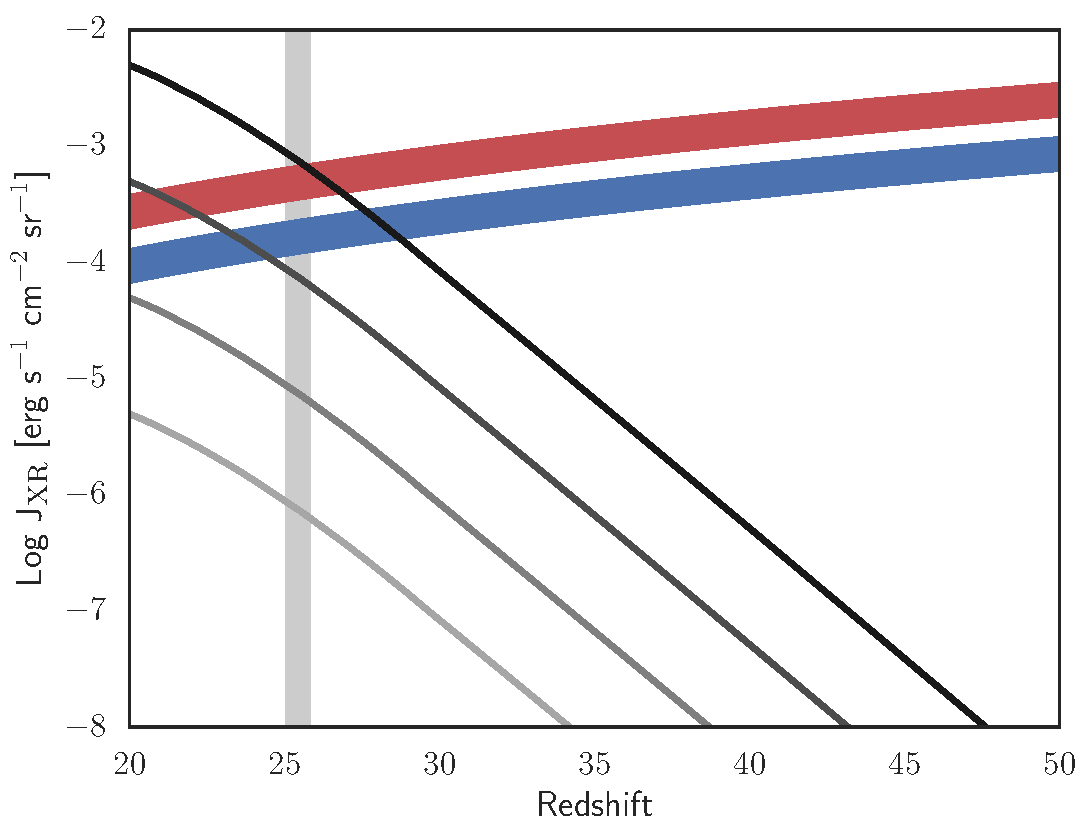
\includegraphics[width=\columnwidth]{figures/J_xr}
   \caption{X-ray average intensity as a function of redshift. The
     lightest grey line represents our fiducial model $J_0$, with successively darker grey lines denoting 10, 100, and $1000\,J_0$, respectively. The blue and red ranges denote the critical intensity above which collapse of the baryonic component into a $2\times10^5\msun$ and $10^6\msun$ halo is suppressed, respectively. In each case, the upper limit of the range assumes the contribution from secondary ionisation is negligible, while the lower limit denotes denotes \jcrit for maximally effective secondary ionisation. The vertical grey bar denotes the range of redshifts over which our minihaloes first reach $n=10^{12}\cc$.}
   \label{xrayIntensity}
 \end{center}
\end{figure}

\begin{figure}
\begin{center}
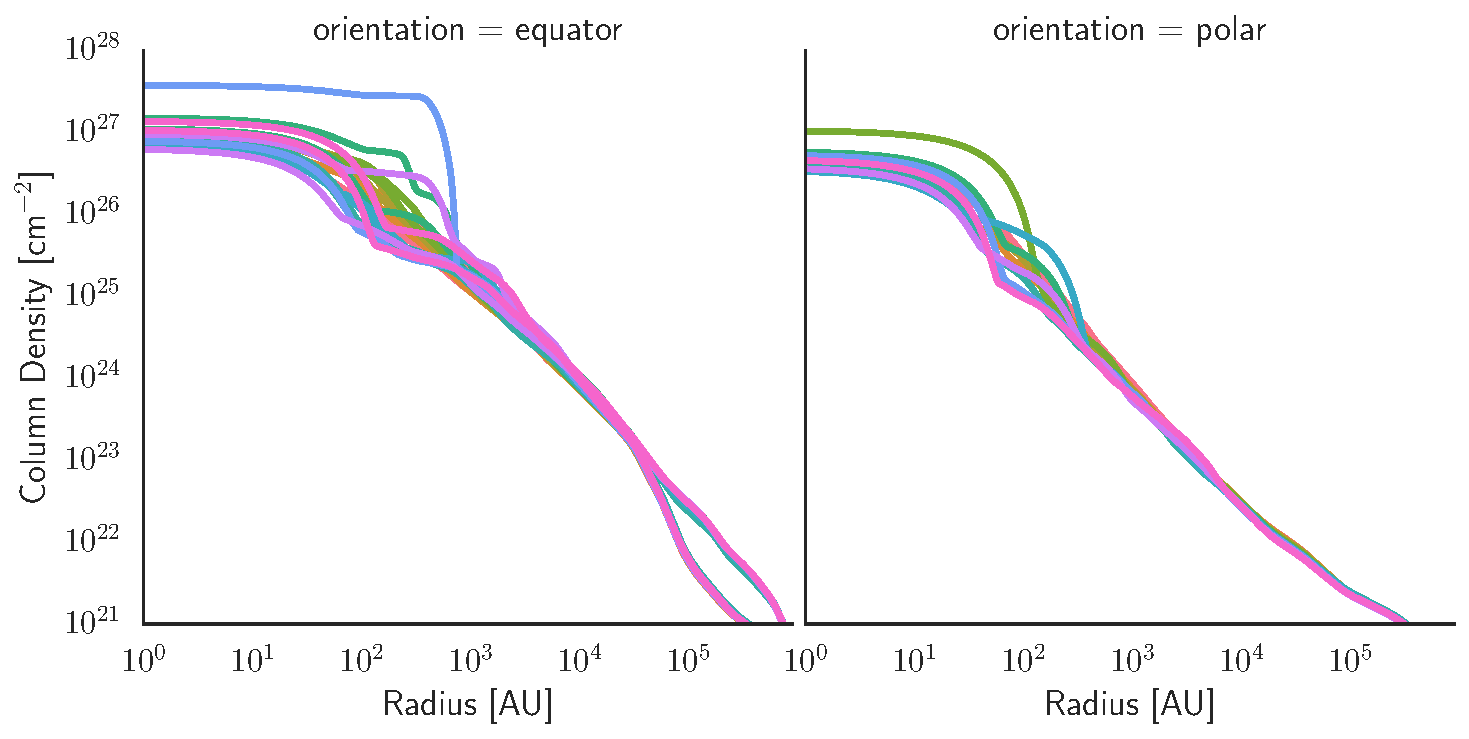
\includegraphics[width=\columnwidth]{figures/optical_depth/column_density}
\caption{\label{fig:column_density} Cumulative column density along both polar and equatorial lines of sight approaching the centre of the minihalo.  Shown is the column density for a selection of snapshots from just prior to the formation of the first sink particle to $5000\yr$ later, with different colors indicating different snapshots.  Note that the scatter in the central $10^3\au$ is larger in the equatorial plane than along the pole: as the accretion disc rotates, occasionally a sink particle orbiting the density-averaged centre lands within the chosen line of sight.}
\end{center}
\end{figure}

%::::::::::::::::::::::::::::::::::::::::::::::::::::::::::::::::::::::::::::::
\subsection{Jeans Mass Filtering under X-ray Feedback}
\label{filtering}
The presence of an ionising X-ray background will necessarily heat the
gas in the IGM.  As a result, collapse into a minihalo will be
suppressed when the thermal energy of the gas exceeds the
baryonic gravitational potential energy of the minihalo in question.  The
baryonic gravitational potential energy of a minihalo prior to collapse is given by
\begin{equation}
  \left|\egrav\right| \simeq \frac{\Omega_B}{\Omega_m} \frac{G \mvir^2}{\rvir},
\end{equation}
where $G$ is the gravitational constant, \mvir is the virial mass, and \rvir is the virial radius of the minihalo.
The gas in the minihalo will naturally undergo adiabatic heating as it
is compressed, but the cooling provided by the formation of molecular hydrogen keeps this process from halting collapse.  An additional heating
mechanism, provided here by X-rays, is required to prevent dissipational collapse of the gas.  We approximate this
excess thermal energy \etherm as
\begin{equation}
  \etherm \simeq \gxr \tff \rvir^3,
\end{equation}
where \gxr is the X-ray heating rate per unit volume and \tff is the freefall
time on which gravity draws gas into the minihalo, given by
\begin{equation}
  \tff = \sqrt{\frac{3\pi}{32 G \rho_{\mathrm b}}},
\end{equation}
where $\rho_{\mathrm b}$ is the background density. To first order then, the critical heating rate \gcrit for suppressing collapse  is  given by
\begin{equation}
  \gcrit = \frac{\Omega_B}{\Omega_m} \frac{G \mvir^2}{\tff \rvir^4}.
\end{equation}
Utilising the fact that 
\begin{equation}
  \mvir \simeq \frac{4\pi}{3}\rvir^3 (200 \rho_{\mathrm b})
\end{equation} 
and
\begin{equation}
  \rho_{\mathrm b} = \rho_0 (1+z)^3,
\end{equation}
where $\rho_0 = 2.5\times10^{-30}\,{\mathrm g}\cc$ is the average matter density at the present epoch, we can solve for \gcrit as a function of halo mass and redshift:
\begin{equation}
  \begin{split}
    \gcrit(M,z) = \; & 1.3\times10^{-28} \erg\s^{-1}\cc \\  
    &\times \left(\frac{M}{10^6\msun}\right)^{\frac{2}{3}} 
    \left(\frac{1+z}{20}\right)^{\frac{11}{2}},
  \end{split}
\end{equation}
where we have normalised to typical minihalo values.  

Prior to minihalo virialisation, gas densities are relatively low, such that attenuation of the CXB as it penetrates the minihalo is negligible (see \RefFig{fig:khratesXR}). Given this, \gxr
is related to the intensity of the CXB as follows:
\begin{equation}
\gxr = 4\pi n \int_{\nu_{\mathrm min}}^{\nu_{\mathrm max}} \jxrvz \sigma_{\nu}
\left(1 - \frac{\nu_{\mathrm ion}}{\nu} \right) d\nu + \Gamma_{\textsc{xr}, \mathrm sec},
\end{equation}
where $n$ is the gas number density and $\Gamma_{\textsc{xr}, \mathrm sec}$ is the contribution to the heating rate from secondary ionisation. While the contribution of secondary ionisation events to the heating rate has a complicated dependence on the ionisation fraction \citep[][see \RefSec{xrays} for details]{ShullvanSteenberg1985}, $\Gamma_{\textsc{xr}, \mathrm sec}$ never enhances \gxr by more than a factor of two in the regime considered here.  When secondary ionisation heating is negligible, 
we can similarly estimate the critical X-ray background required to suppress collapse:
\begin{equation}
  \begin{split}
    \jcrit(M,z) = \; & 3.4 \times 10^{-4} \erg\s^{-1} \cm^{-2} \sr^{-1}\\ &\times \left(\frac{M}{10^6\msun}\right)^{\frac{2}{3}}
    \left(\frac{1+z}{20}\right)^{\frac{5}{2}}.
  \end{split}
\end{equation}
When secondary ionisation heating is maximally effective then, \jcrit will be a factor of two lower. Both limits for \jcrit are shown in \RefFig{xrayIntensity} for both a $10^6$  and a $2\times10^5\msun$ minihalo.  These can be interpreted as the approximate range in which the CXB will begin to have a significant impact on the collapse of gas into such a minihalo.


%==============================================================================
\section{Numerical Methodology}
\label{methods}
%::::::::::::::::::::::::::::::::::::::::::::::::::::::::::::::::::::::::::::::
\subsection{Initial Setup}
\label{setup}
We use the well-tested $N$-body smoothed particle hydrodynamics (SPH) code \textsc{gadget-2} \citep{Springel2005}. We initialised our simulations in a periodic box of length 140 kpc (comoving) at $z=100$ in accordance with a $\Lambda$CDM model of hierarchical structure formation. An artificially enhanced normalisation of the power spectrum, $\sigma_8 = 1.4$, was used to accelerate structure formation. See \citet{StacyGreifBromm2010} for a discussion of the validity of this choice. High resolution in this simulation was achieved using a standard hierarchical zoom-in technique for both DM and SPH particles. Three nested levels of additional refinement at 40, 30 and 20 kpc (comoving) were added, each centred on the point where the first minihalo forms in the simulation.  As resolution increases, each `parent' particle is replaced by eight `child' particles, such that at the greatest refinement level, each original particle has been replaced by 512 high-resolution particles.  These highest-resolution SPH particles have a mass $m_{\textsc{sph}} = 0.015\msun$, such that the mass resolution of the simulation is $M_{\mathrm res} \simeq 1.5 N_{\mathrm neigh} m_{\textsc{sph}} \lesssim 1\msun$, where $N_{\mathrm neigh} \simeq 32$ is the number of particles used in the SPH smoothing kernel \citep{BateBurkert1997}.

%::::::::::::::::::::::::::::::::::::::::::::::::::::::::::::::::::::::::::::::
\subsection{Thermodynamics and Chemistry}
\label{chemistry}
Our chemistry and cooling network is the same as that described in \citet{Greifetal2009b}.  We follow the abundances of \h, \hplus, \hminus, \htwo, $\htwo^+$, \he, \heplus, $\he^{++}$, \deut, $\deut^+$, \hd and e$^-$.  All relevant cooling mechanisms, including cooling via \h and \he collisional excitation and ionisation, recombination, bremsstrahlung and inverse Compton scattering are accounted for.  Of particular importance is cooling via the ro-vibrational modes of \htwo, which are excited by collisions with \h and \he atoms and other \htwo molecules.  At high densities, additional \htwo processes must also be included in order to properly model the gas evolution.  For example, three-body \htwo formation and the associated heating becomes important above $n\gtrsim10^8$\cc \citep{Turketal2011}.  The formation rates for these reactions are uncertain; we employ the intermediate rate from \citet{PallaSalpeterStahler1983}. At densities greater than \about$10^9\cc$, the ro-vibrational lines for \htwo become optically thick, decreasing the efficiency of such cooling. We employ the Sobolev approximation and an escape probability formalism to account for this (see \citealt{Yoshidaetal2006, Greifetal2011} for details).

%::::::::::::::::::::::::::::::::::::::::::::::::::::::::::::::::::::::::::::::
\subsection{Optical Depth Estimation}
\label{attenuation}
Over the length scale of our cosmological box, the X-ray optical depth of primordial gas is $\ll 1$ everywhere except approaching the centre of the star-forming minihalo. As the CXB radiation penetrates the minihalo, it will necessarily be attenuated due to the high column density $N$ of the intervening gas.  In order to estimate the optical depth, we directly calculate the column density approaching the centre of the accretion disc along both polar and equatorial lines of sight in the absence of a CXB. As shown in Figure \ref{fig:column_density}, the column density remains essentially constant for the duration of the simulation, and has a simple power-law dependence on radius over several orders of magnitude up to the resolution limit of our simulation ($\sim100\au$). This same power-law behaviour can be seen versus density as well, as shown in Figure \ref{fig:ncol_fit}. In addition we notice that for a given gas density, the column density along the pole is roughly a factor of 10 lower than along the equator.  Performing an ordinary least squares fit to the combined data from several snapshots for $n > 10^4\cc$, we find that the column density along the pole and equator is well fit by 
\begin{equation}
{\mathrm log}_{10}(N_{\mathrm \small pole}) = 0.5323\, {\mathrm log_{10}}(n) + 19.64
\end{equation}
and
\begin{equation}
{\mathrm log}_{10}(N_{\mathrm \small eq}) = 0.6262\, {\mathrm log_{10}}(n) + 19.57, 
\end{equation}
respectively, and does not change appreciably with increasing \jxr.

\begin{figure}
\begin{center}
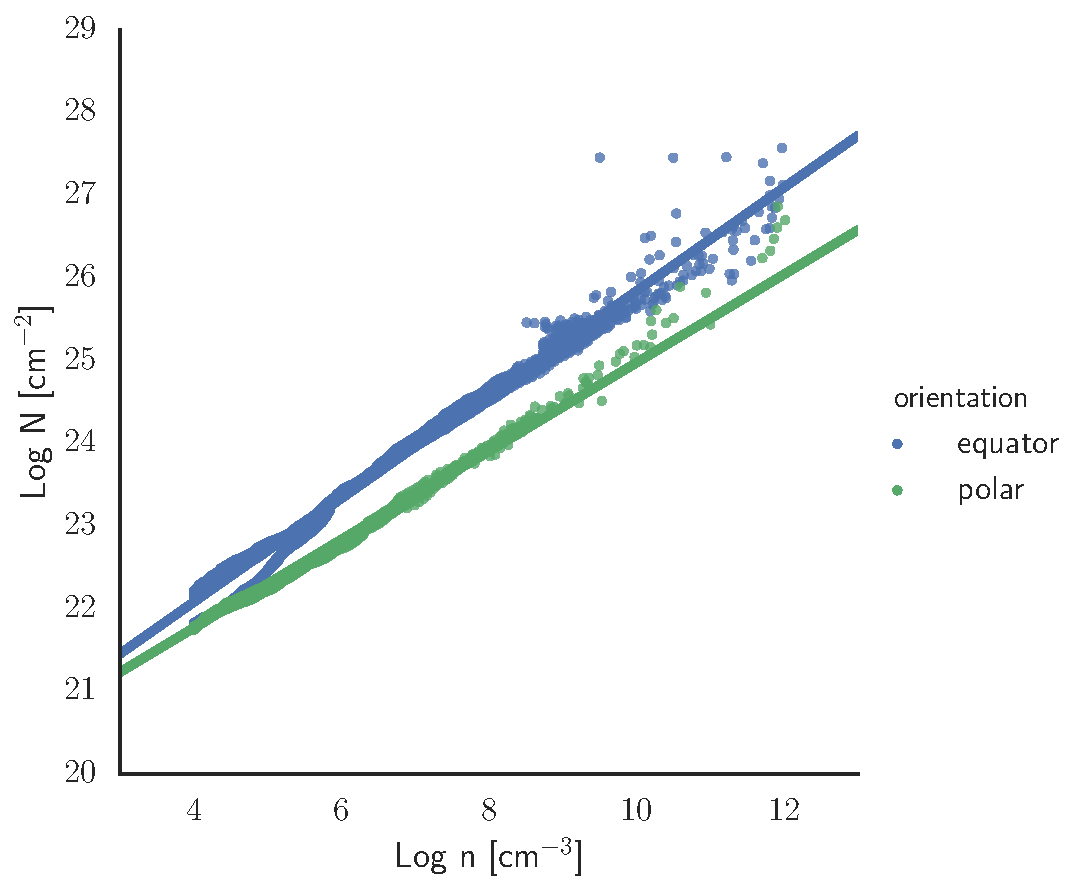
\includegraphics[width=\columnwidth]{figures/optical_depth/col_density_fit}
\caption{\label{fig:ncol_fit}
Column density as a function of gas number density along both polar (green) and equatorial (blue) lines of sight.  Points sample the distribution of column density as a function of number density for their respective lines of sight across several snapshots, while the lines indicate the $\chi^2$ best fit.}
\end{center}
\end{figure}

To account for this difference in column density, we assume every line of sight within 45 degrees of the pole \citep{Hosokawaetal2011} experiences column density $N_{\mathrm \small pole}$ and every other line of sight experiences $N_{\mathrm \small eq}$. Radiation within the opening angle is attenuated by $e^{-\sigma_{\nu}^i N_{\mathrm \small pole}}$ while the remainder of the background is attenuated by $e^{-\sigma_{\nu}^i N_{\mathrm \small eq}}$, allowing us to define an effective optical depth $\tau_{\textsc{xr}}$ such that
\begin{equation}
e^{-\tau_{\textsc{xr}}} = \frac{2 \Omega_{\mathrm \small pole}}{4\pi} e^{-\sigma_{\nu}^i N_{\mathrm \small pole}} + \frac{4\pi - 2 \Omega_{\mathrm \small pole}}{4\pi} e^{-\sigma_{\nu}^i N_{\mathrm \small eq}},
\end{equation}
\citep[e.g.,][]{ClarkGlover2014}.
Here we use the standard expressions for the photoionisation cross sections $\sigma^i_{\nu}$ of hydrogen and helium \citep[e.g.,][]{BarkanaLoeb2001, OsterbrockFerland2006} and define $\Omega_{\mathrm \small pole}$ as
\begin{equation}
\Omega_{\mathrm \small pole} = \int_0^{2\pi}{\mathrm d}\phi \int_0^{\pi/4}{\mathrm sin}\theta \,{\mathrm d}\theta
						 = 1.84\,{\mathrm sr}.
\end{equation}
Accounting for this attenuation and incorporating the cosmic X-ray background described in Section \ref{HMXB}, the resulting ionisation and heating rates for the $\jxr=J_0$ case at $z=25$ as a function of total number density are shown in Figure \ref{fig:khratesXR}.


\begin{figure}
\begin{center}
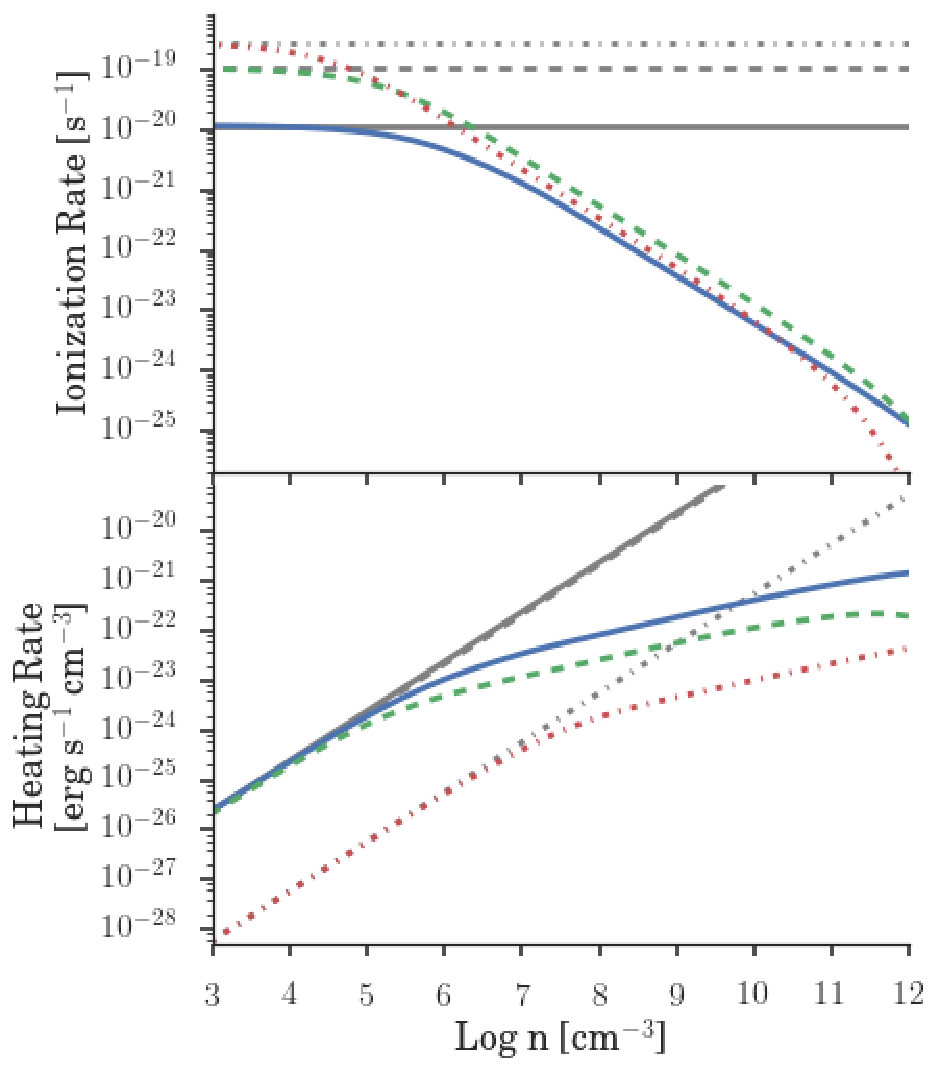
\includegraphics[width=\columnwidth]{figures/khrates/khratesXR}
\caption{\label{fig:khratesXR}
X-ray ionisation and heating rates for \HI, \HeI and \HeII as a function of total number density for the $\jxr=J_0$ case at $z=25$. In both panels, the solid blue, dashed green, and dash-dotted red lines denote \HI, \HeI, and \HeII, respectively.  The grey lines in each style demonstrate the expected rates in the absence of X-ray self-shielding for that species.  \HI dominates both ionisation and heating when the relative abundances of these species are accounted for, and we see that X-rays penetrating the minihalo experience significant attenuation above densities of $n\sim10^6\cc$.}
\end{center}
\end{figure}

%::::::::::::::::::::::::::::::::::::::::::::::::::::::::::::::::::::::::::::::
\subsection{X-ray Ionisation and Heating}
\label{xrays}
To study the effects of X-ray ionisation and heating on primordial star formation, we implement a uniform CXB as discussed in \RefSec{HMXB}. For further details, see \citet{Jeonetal2012, Jeonetal2014a}. Accounting for attenuation of the incident X-ray radiation while penetrating the minihalo, the primary ionisation rate coefficient for chemical species $i$ can be written as 
\begin{equation}
k^i_{\mathrm ion, p} = 4\pi \int_{\nu_{\mathrm min}}^{\nu_{\mathrm max}}
\frac{J_{\nu} \sigma^i_{\nu}}{h \nu} e^{-\tau_{\textsc{xr}}} d\nu
\end{equation}
where $\nu_{\mathrm min} = 1\kev/h$ and $\nu_{\mathrm max} = 10\kev/h$.  

We include the effects of secondary ionisation from energetic electrons released by the absorption of X-ray photons by adopting the fitting formulae of Shull \& van Steenberg (\citeyear{ShullvanSteenberg1985}; see also \citealt{ValdesFerrara2008, FurlanettoStoever2010}), who calculated the fractions of the initial electron energy going into heating the surrounding gas, as well as into secondary ionisations of \HI and \HeI ($f_{\mathrm H}$ and $f_{\mathrm He}$, respectively). While such secondary ionisation events have a significant impact on the ionisation fraction of \HI and \HeI, secondary ionisations of \HeII are negligible \citep{ShullvanSteenberg1985}, and are not included here.  The effective ionisation rates are thus given by
\begin{equation}
k^i_{\mathrm ion} = k^i_{\mathrm ion, p} + k^i_{\mathrm ion, sec}
\end{equation}
where
\begin{equation}
k^{\mathrm \HI}_{\mathrm ion, sec} = f_{\mathrm H} \left( \Gamma_{\mathrm \HI} + \frac{n_{\mathrm \HeI}}{ n_{\mathrm \HI}} \Gamma_{\mathrm \HeI} \right) \frac{1}{13.6\ev}
\end{equation}
and
\begin{equation}
k^{\mathrm \HeI}_{\mathrm ion, sec} = f_{\mathrm He} \left( \Gamma_{\mathrm \HeI} + \frac{n_{\mathrm \HI}}{ n_{\mathrm \HeI}} \Gamma_{\mathrm \HI} \right) \frac{1}{24.6\ev}.
\end{equation}
Here $\Gamma_i$ is the heating rate at which excess energy from the initial X-ray photoionisation is released into the gas, given by
\begin{equation}
\Gamma_i = 4\pi n_i \int_{\nu_{\mathrm min}}^{\nu_{\mathrm max}} J_{\nu} \sigma^i_{\nu}
\left(1 - \frac{\nu^i_{\mathrm ion}}{\nu} \right) e^{-\tau_{\textsc{xr}}} d\nu,
\end{equation} 
where $\nu^i_{\mathrm ion}$ is the ionisation threshold of the species in question; $h\nu_{\mathrm ion} = 13.6\ev$, 24.6\ev and 54.4\ev for hydrogen, neutral helium and singly ionised helium, respectively.

The fraction of the initial electron energy going into secondary ionisations depends on the hydrogen ionisation fraction $x_{\mathrm ion, H}$ as follows:
\begin{equation}
f_{\mathrm H} = 0.3908 \left( 1 - x_{\mathrm ion, H}^{0.4092} \right) ^{1.7592}
\end{equation}

\begin{equation}
f_{\mathrm He} = 0.0554 \left( 1 - x_{\mathrm ion, H}^{0.4614} \right) ^{1.6660}.
\end{equation}
Thus the total heating rate $\Gamma_i^{\mathrm tot}$, including contributions from both primary and secondary ionizations, can be written as
\begin{equation}
\Gamma_i^{\mathrm tot} = 4\pi n_i \left(1 - f_i \right)
\int_{\nu_{\mathrm min}}^{\nu_{\mathrm max}} J_{\nu} \sigma^i_{\nu}
\left(1 - \frac{\nu^i_{\mathrm ion}}{\nu} \right) e^{-\tau_{\textsc{xr}}} d\nu.
\end{equation}

\begin{figure}
  \begin{center}
    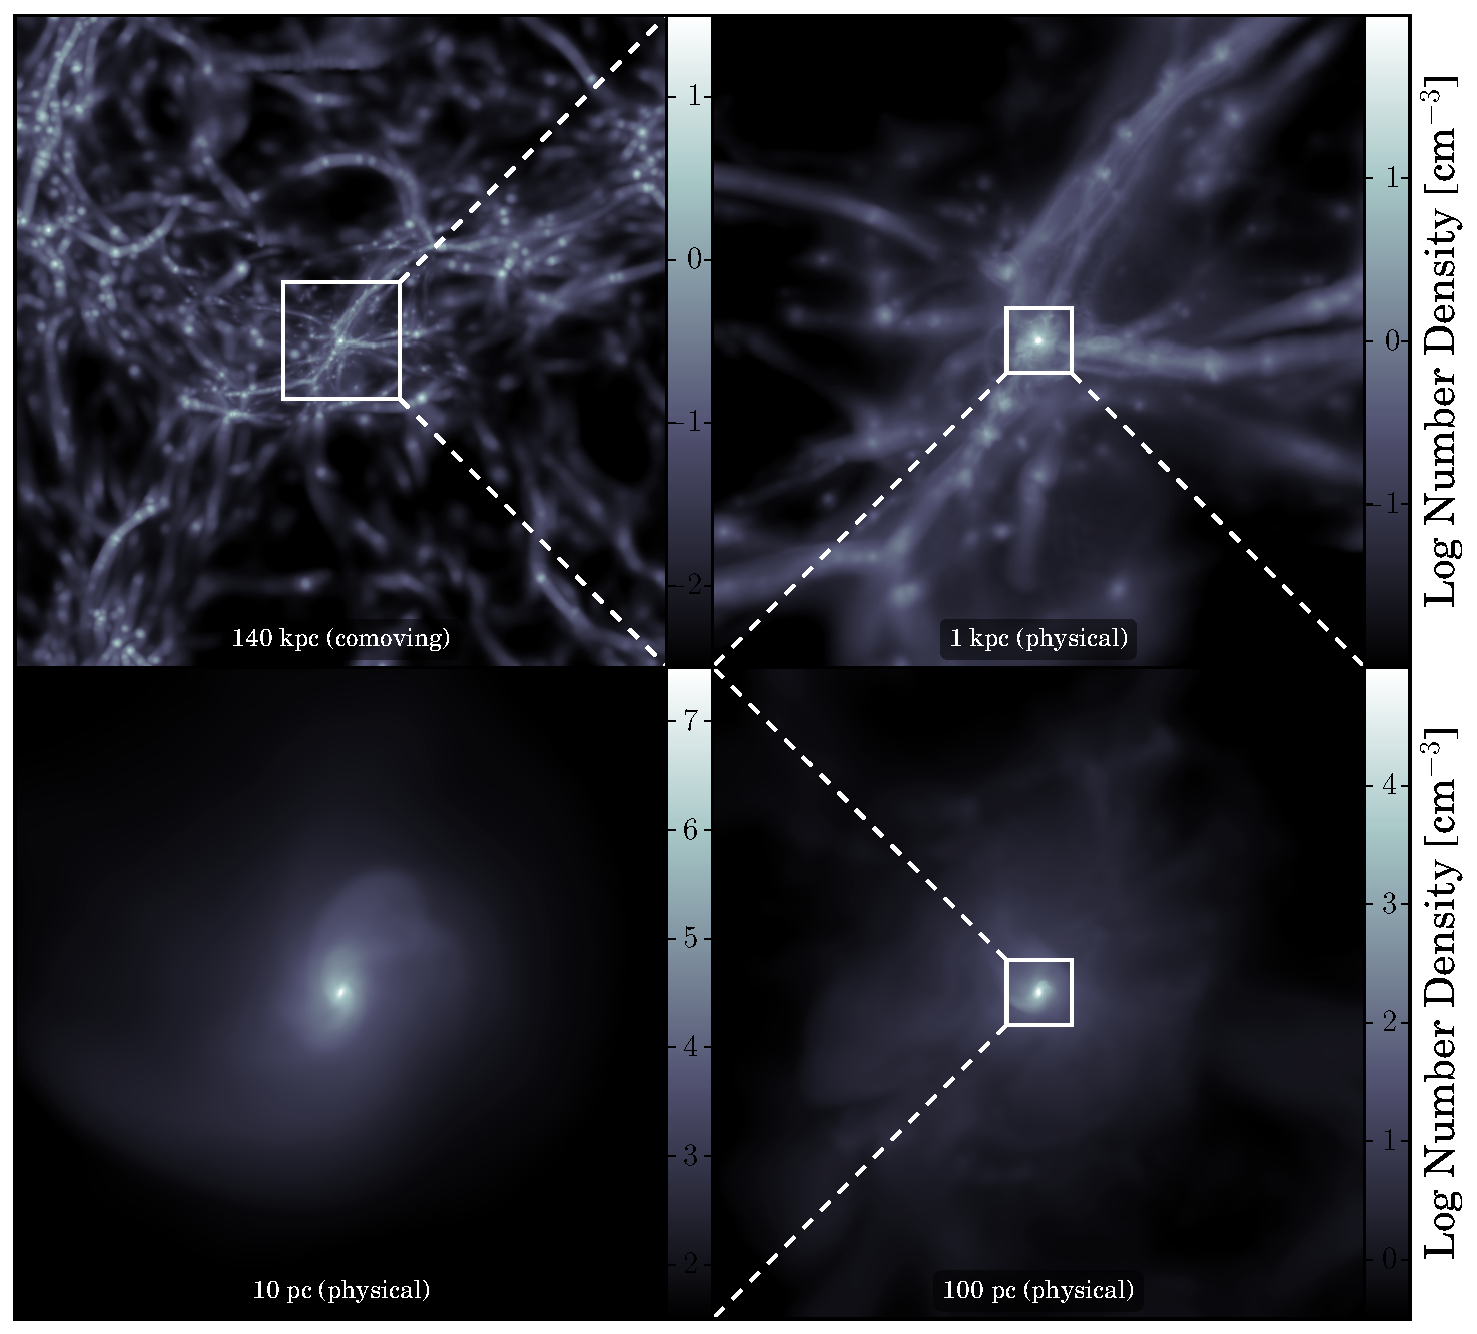
\includegraphics[width=0.67\textwidth]{figures/structure/structure-vanilla_t0}
    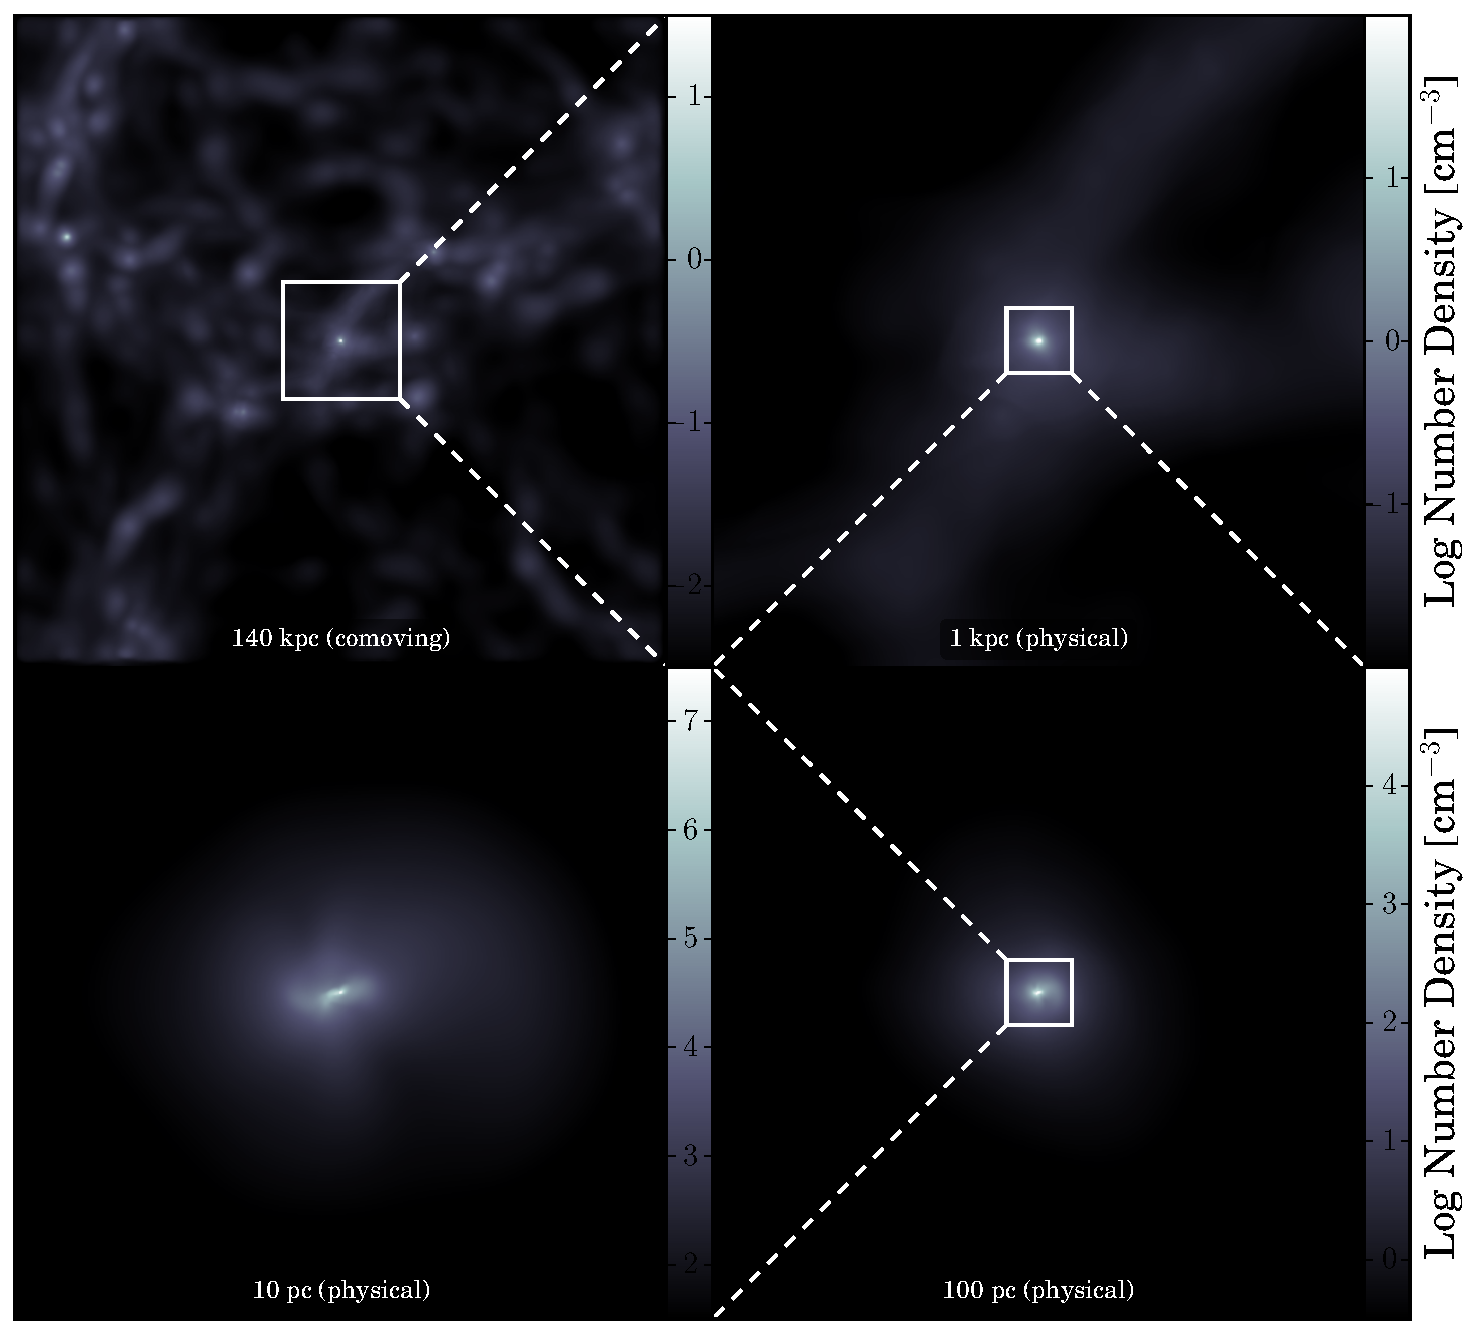
\includegraphics[width=0.67\textwidth]{figures/structure/structure-xr_tau2_J2_t0}
    \caption{Density projection of the final simulation output 5000\yr after the formation of the first sink particle on progressively smaller scales for both the $\jxr=0$ (top) and the shielded $\jxr=10^2\,J_0$ (bottom) simulations.  White boxes indicate the region depicted on the next smaller scale.  Clockwise from top left: full simulation box; minihalo and surrounding filamentary structure; central 100\pc of minihalo; central 10\pc.  The density scale for each panel is included just to the right -- note that the scaling changes from panel to panel. In both cases, note how the morphology approaches an increasingly smooth, spherical distribution on the smallest scales, where the gas is in quasi-hydrostatic equilibrium.  In the shielded $\jxr=10^2\,J_0$ case, the low-density filamentary structure is smoothed out due to X-ray heating, whereas gas at high densities is shielded and proceeds to collapse unimpeded.}
    \label{zoom-in}
  \end{center}
\end{figure}

\begin{figure}
  \begin{center}
    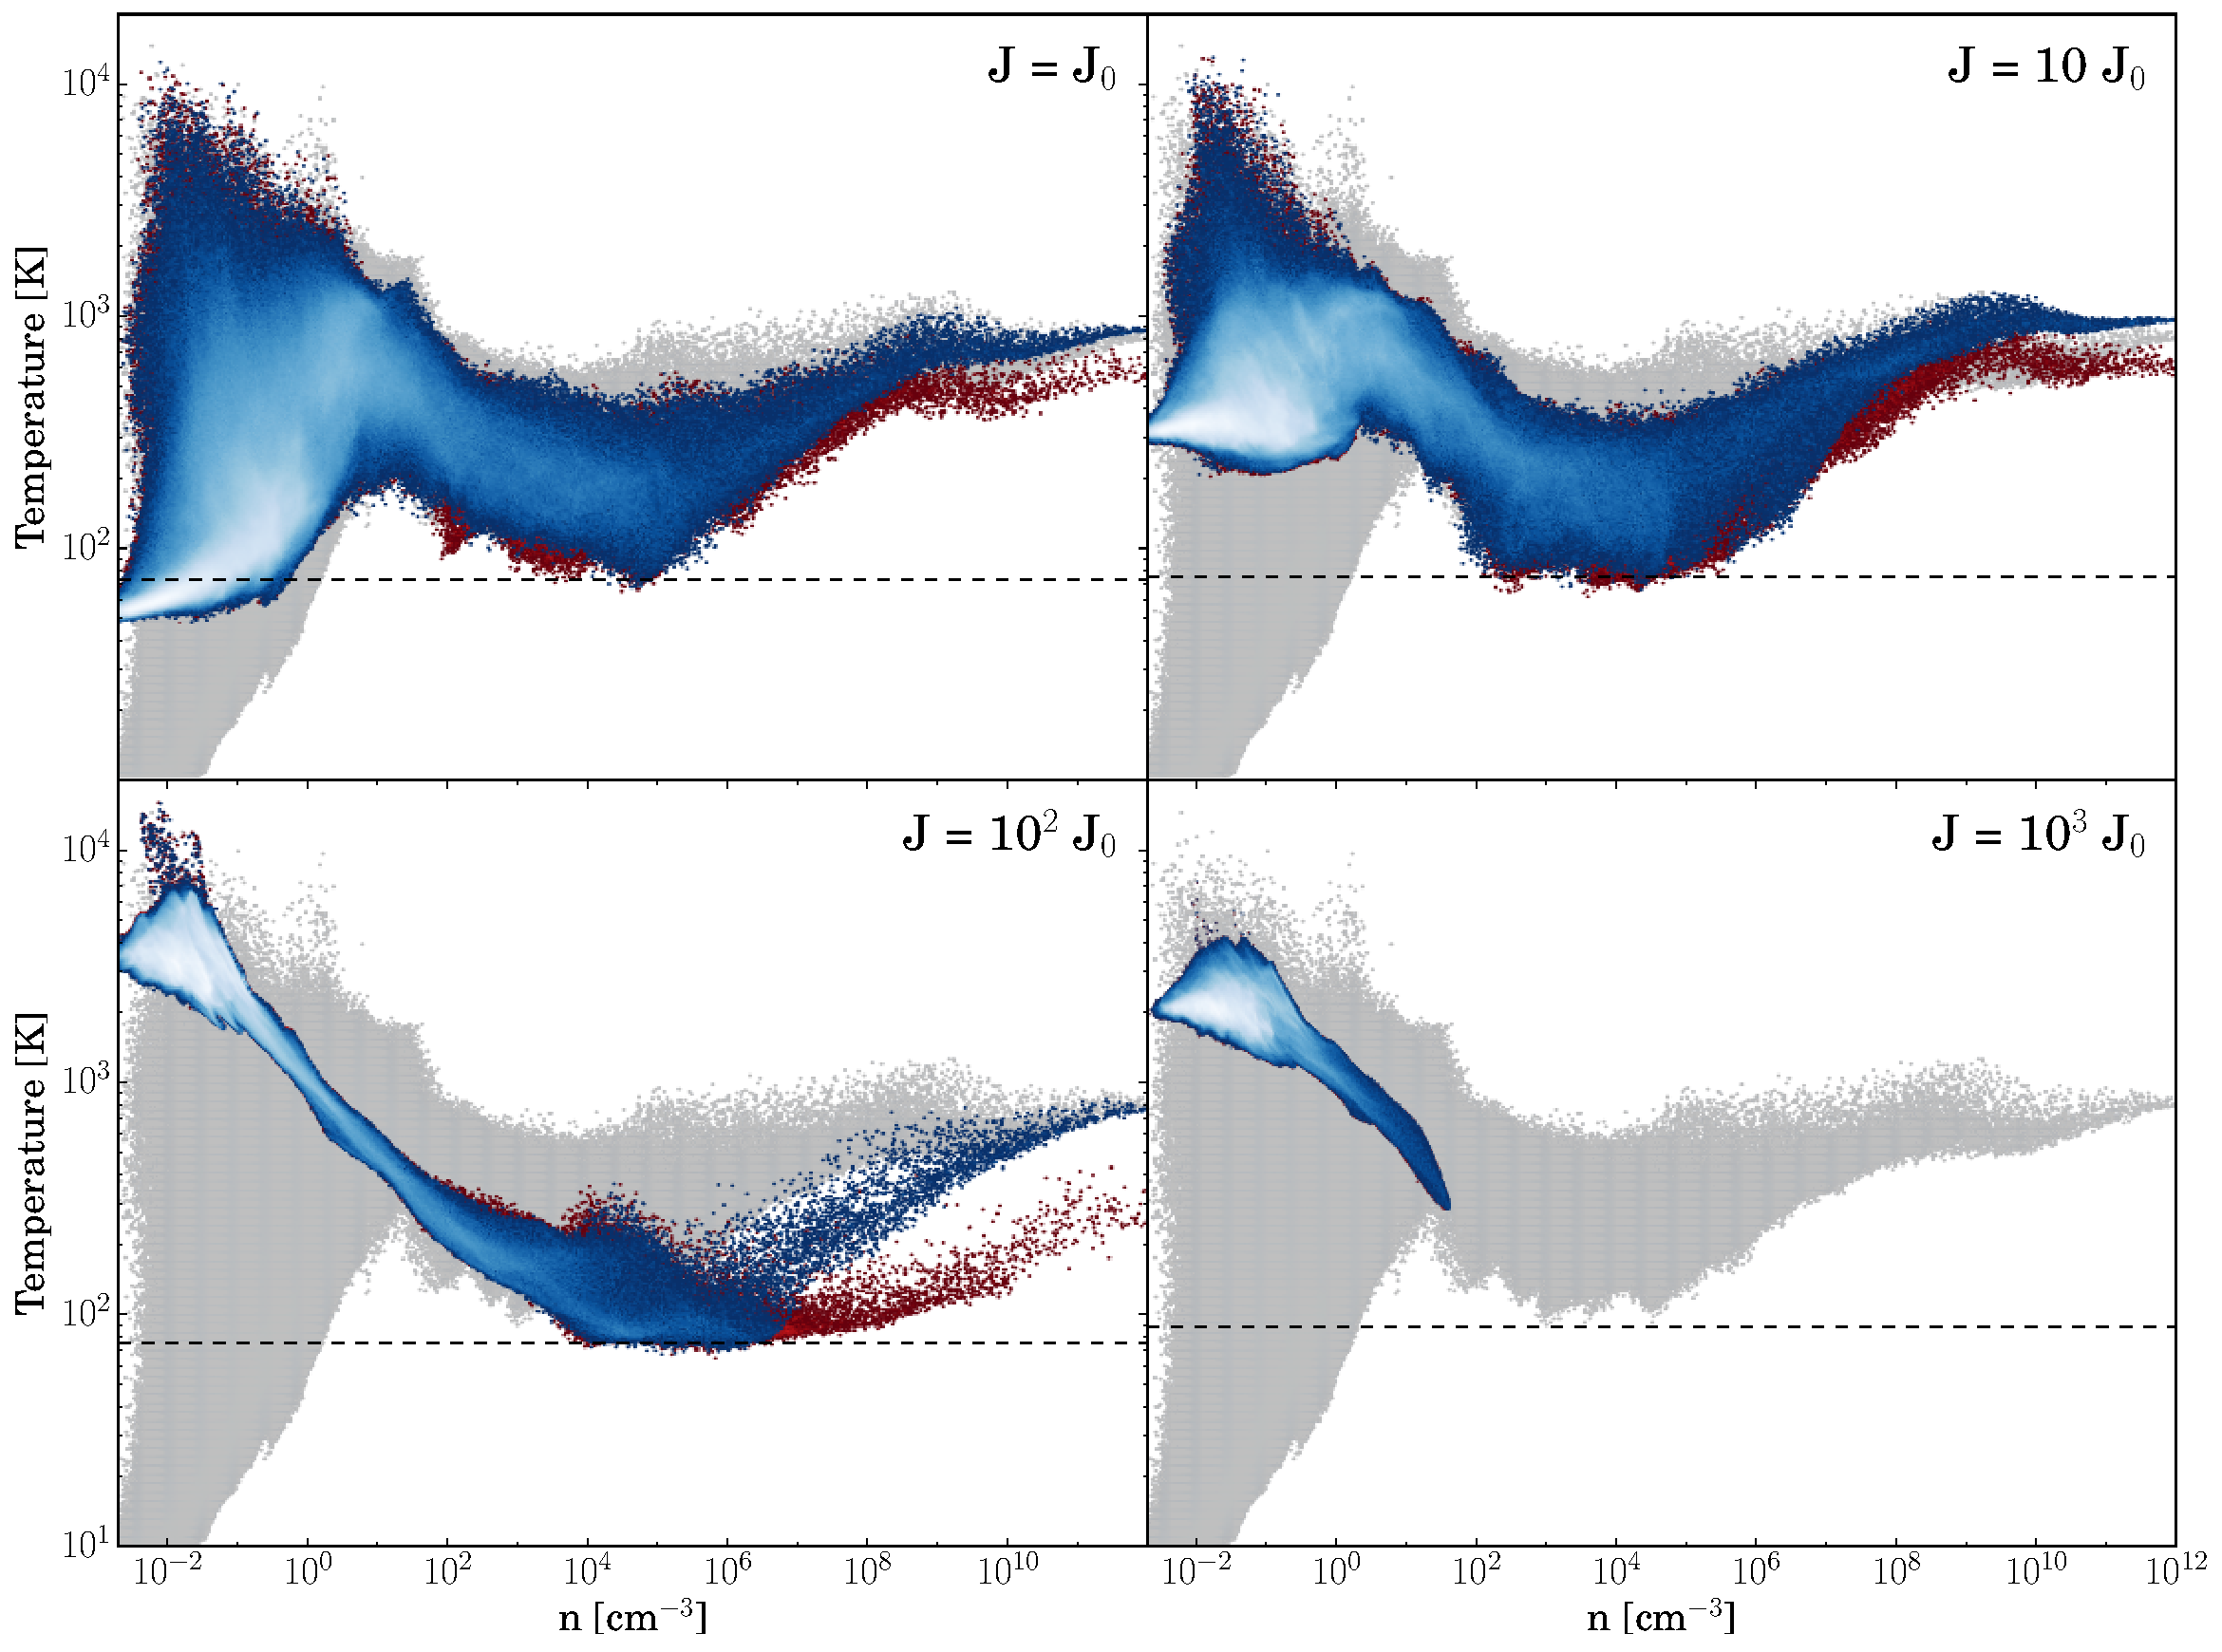
\includegraphics[width=\columnwidth]{figures/phase_diagrams/temp}
    \caption{Mass-weighted temperature distribution of the collapsing gas in each simulation, shown just prior to sink formation---or maximum density reached in the case of the $10^3 J_0$ background. Each panel shows the behaviour of the gas in the presence of the CXB, both shielded (in blue) and unshielded (in red). For comparison, the gas behaviour in the $\jxr=0$ case is shown in grey.  Dashed lines denote the CMB temperature. All simulations except the $10^3 J_0$ case successfully collapse to high densities.  Gas at low densities gets progressively hotter and gas in the loitering phase gets progressively cooler with increasing \jxr. Note that in all cases where the minihalo successfully proceeds to collapse, the shielded gas re-converges to the $\jxr=0$ case prior to reaching sink formation densities.}
    \label{Tdens}
  \end{center}
\end{figure}
%::::::::::::::::::::::::::::::::::::::::::::::::::::::::::::::::::::::::::::
\subsection{Sink Particles}
\label{sink_particles}
We employ the sink particle method described in \citet{StacyGreifBromm2010}.  When the density of a gas particle exceeds $n_{\mathrm max} = 10^{12}\cc$, we replace it and all non-rotationally-supported particles within the accretion radius $r_{\mathrm acc}$ with a single sink particle.  We set $r_{\mathrm acc}$ equal to the resolution length of the simulation: $r_{\mathrm acc} = L_{\mathrm res} \simeq 50\au$.  Here, 
\begin{equation}
L_{\mathrm res} \simeq 0.5 \left( \frac{M_{\mathrm res}}{\rho_{\mathrm max}} \right)^{1/3},
\end{equation}
where $\rho_{\mathrm max} = n_{\mathrm max} m_{\mathrm H}$.  The sink thus immediately accretes the majority of the particles within its smoothing kernel, such that its mass $M_{\mathrm sink}$ is initially close to $M_{\mathrm res} \simeq 1\msun$. Once the sink is formed, additional gas particles and smaller sinks are accreted as they approach within $r_{\mathrm acc}$ of that sink particle.  After each accretion event, the position and momentum of the sink particle is set to the mass-weighted average of the sink and the accreted particle.

Following the creation of a sink particle, its density, temperature and chemical abundances are no longer updated. The sink's density is held constant at $10^{12}\cc$, and its temperature is kept at 650\kelvin, typical for collapsing gas reaching this density; the pressure of the sink is set correspondingly. Assigning a temperature and pressure to the sink particle in this fashion allows it to behave as an SPH particle. This  avoids the creation of an artificial pressure vacuum, which would inflate the accretion rate onto the sink \citep[see][]{BrommCoppiLarson2002, MartelEvansShapiro2006}. The sink's position and momentum continue to evolve through gravitational and, initially, hydrodynamical interactions with the surrounding particles. As it gains mass and gravity becomes the dominant force, the sink behaves less like an SPH particle and more like a non-gaseous $N$-body particle.

%==============================================================================
\section{Results}
\label{results}
We perform a total of nine simulations, following each for 5000 years after the formation of the first sink particle in the simulation.  Beyond our fiducial case of $\jxr=J_0$ and the standard case of $\jxr=0$, we examine three additional  simulations with $\jxr = 10$, $10^2$, and $10^3$ times $J_0$. The results of a $\jxr = 10^{-1}\,J_0$ simulation were indistinguishable from $\jxr=0$. Not only is the CXB at high redshifts subject to fairly large uncertainties, but as Pop III star formation is highly biased there is likely a significant amount of cosmic variance.
In addition, we also consider the optically-thin limit where $\tau_{\textsc{xr}} \rightarrow 0$.  While physically unrealistic, these numerical experiments serve as comparison cases to more fully elucidate the physics in the properly shielded simulations.

%::::::::::::::::::::::::::::::::::::::::::::::::::::::::::::::::::::::::::::::
\subsection{Initial Collapse}
\label{collapse}
\subsubsection{Collapse under Enhanced Cooling}
\label{collapse_acceleration}
\RefFig{zoom-in} shows the final simulation output on various scales for both the $\jxr=0$ and the shielded $\jxr = 10^2\,J_0$ case.  While the expected filamentary structure is visible in all cases, the effects of X-ray heating in the  $\jxr = 10^2\,J_0$ case are readily apparent, with the low-density filamentary gas  
experiencing significant heating. With the usual definition of the virial radius \rvir as $\rho = \rho_{\mathrm vir} \equiv 178\,\rho_{\mathrm b}$, where $\rho$, $\rho_{\mathrm vir}$ and $\rho_{\mathrm b}$ are the average halo density, the density at the point of virialisation and the background density at the time of halo virialisation, we find that our $\jxr = 0$ minihalo collapses at $z=25.04$ with $\rvir \simeq 85\pc$ and $\mvir \simeq 2.1\times10^5\msun$, typical for the minihalo environment \citep{Bromm2013}.  

\begin{figure}
  \begin{center}
    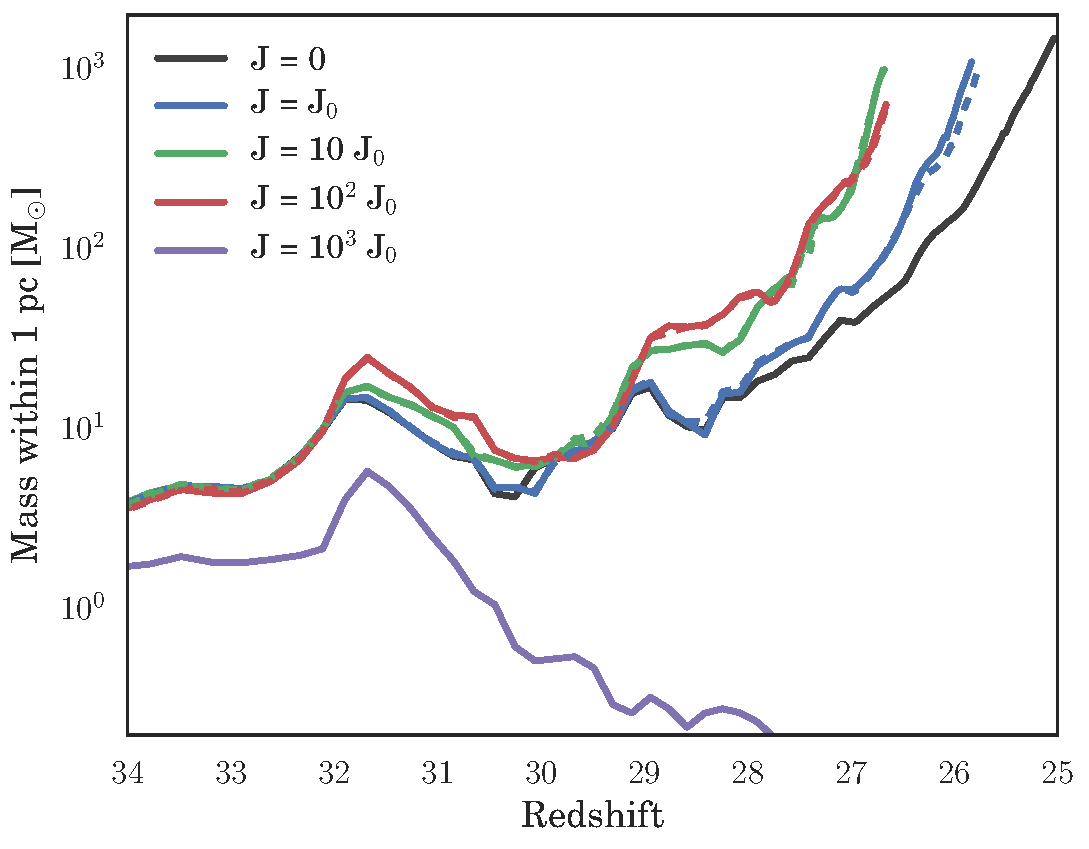
\includegraphics[width=\columnwidth]{figures/growth/collapse}
    \caption{Total gas mass within 1\pc of the highest density point in each simulation over cosmic time. Shielded simulations are denoted by solid lines, unshielded simulations by dashed lines.  Both with and without shielding, as \jxr increases, the gas in the loitering phase becomes cooler. This lowers the Jeans mass, allowing the gas to collapse to high densities sooner.}
    \label{fig:collapse}
  \end{center}
\end{figure}

After the minihalo virialises, the gas continues to collapse in accordance with the standard picture of Pop III star formation \citep[e.g.,][]{StacyGreifBromm2010, Greifetal2012, StacyBromm2013}. This picture is modified slightly in the presence of an X-ray background, but in the $\jxr=0$ case the gas heats adiabatically until reaching $n\sim1\cc$, attaining temperatures of $\sim$1000\kelvin. Beyond this point, the gas is able to cool via the ro-vibrational modes of \htwo, reaching a minimum temperature of \about200\kelvin at a density of $n\sim10^4\cc$.  After exiting the quasi-hydrostatic `loitering phase' \citep{BrommCoppiLarson2002}, the gas enters runaway collapse until $n\sim10^8\cc$, when three-body reactions become important.  This process turns the gas fully molecular by $n\sim10^{12}\cc$, the density at which we form sink particles. As seen in \RefFig{Tdens}, this basic picture holds true even as we vary the strength of the CXB by several orders of magnitude. 

We find that X-ray heating dominates at low densities in all cases, while above $n\sim10^2\cc$ the additional cooling catalysed by X-ray ionisation exceeds it; the precise density at which this transition occurs depends on the strength of the CXB.  This enhanced cooling significantly impacts the subsequent evolution of the gas as it collapses to high densities; the minimum temperature of the gas in the loitering phase approaches the CMB floor as $\jxr$ increases, and---in the unshielded simulations---remains cooler than the $\jxr=0$ case in all later stages of the collapse. This allows the gas to more easily fulfil the Jeans criterion and thus collapse sooner, as demonstrated by \RefFig{fig:collapse}.

When shielding is properly accounted for, the gas becomes optically thick to X-rays as it exits the loitering phase and proceeds to runaway collapse (see \RefFig{fig:khratesXR}).  In the absence of continued X-ray ionisation, the free electron fraction decays, re-converging with that of the $\jxr=0$ case.  Consequently, the thermodynamic behaviour of the gas at high densities in the shielded simulations is remarkably similar, even as we vary the CXB strength by several orders of magnitude as shown in Figure \ref{Tdens}. This convergence under a wide range of X-ray backgrounds is similar to the behaviour noted by \citet{StacyBrommLoeb2011a} and \citet{Greifetal2011b} in the presence of dark matter--baryon streaming, though we observe an earlier---rather than a later---collapse.

\subsubsection{Collapse Suppression}
 \label{suppression}
Minihalo collapse in the $\jxr = 1000\,J_0$ case is completely suppressed.  While the gas in the very centre of the minihalo does initially begin to cool via \htwo, this process is quickly overwhelmed by heating from the increasingly strong X-ray background.  Despite reaching densities and temperatures approaching $n \simeq 50\cc$ and $T \simeq 200\kelvin$ this cold core is eventually dissipated as the CXB continues to heat the gas. 
The reason for this suppression is demonstrated clearly in \RefFig{suppressed}, where we have shown the enclosed mass and the Jeans mass as a function of radius for both the $\jxr = 0$ and the $\jxr = 1000\,J_0$ case. Here, we calculate the Jeans mass using the average density and temperature within a given radius, extending out to the virial radius of the halo.  The $\jxr = 0$ case is shown just prior to the formation of the first sink particle in that simulation; the $\jxr = 1000\,J_0$ case is shown at the maximum density reached over the course of the simulation.  While the enclosed mass in the $\jxr = 0$ minihalo exceeds the Jeans mass on all scales, and thus is universally collapsing, the cold core in the $\jxr = 1000\,J_0$ minihalo never gains sufficient mass to exceed the Jeans criterion.

%::::::::::::::::::::::::::::::::::::::::::::::::::::::::::::::::::::::::::::::
\subsection{Sink Particle Formation and Accretion}
\subsubsection{Build-up of a Central Disc}
 \RefFig{sinkmasses} shows the growth over time of all sink particles formed in our simulations, from the formation of the first sink to simulation's end 5000\yr later.  Sink particles are formed when the gas in the centre of the minihalo reaches $10^{12}\cc$, and in all cases a central disc forms within $300\yr$ of the first sink particle, as seen in \RefFig{disks}, where we have shown the density structure of the central $10^4\,$AU of each simulation.  In the absence of any X-ray irradiation, the accretion disc fragments and forms a stable binary system, in agreement with previous studies \citep[e.g.,][]{ StacyGreifBromm2010, Clarketal2011a, Clarketal2011b, Greifetal2011, Greifetal2012}. When self-shielding is properly accounted for, the thermodynamic state of the gas in X-ray irradiated minihaloes is remarkably similar to the $\jxr=0$ case by the time it reaches sink formation densities. The mass distribution, however, is in all cases significantly steeper than in the $\jxr=0$ case, as shown in \RefFig{mbins}. This is a direct consequence of the earlier collapse discussed in \RefSec{collapse_acceleration}: the sooner the gas collapses to high densities, the less time is available for gas to accumulate in the centre of the minihalo. 

\begin{figure}
  \begin{center}
    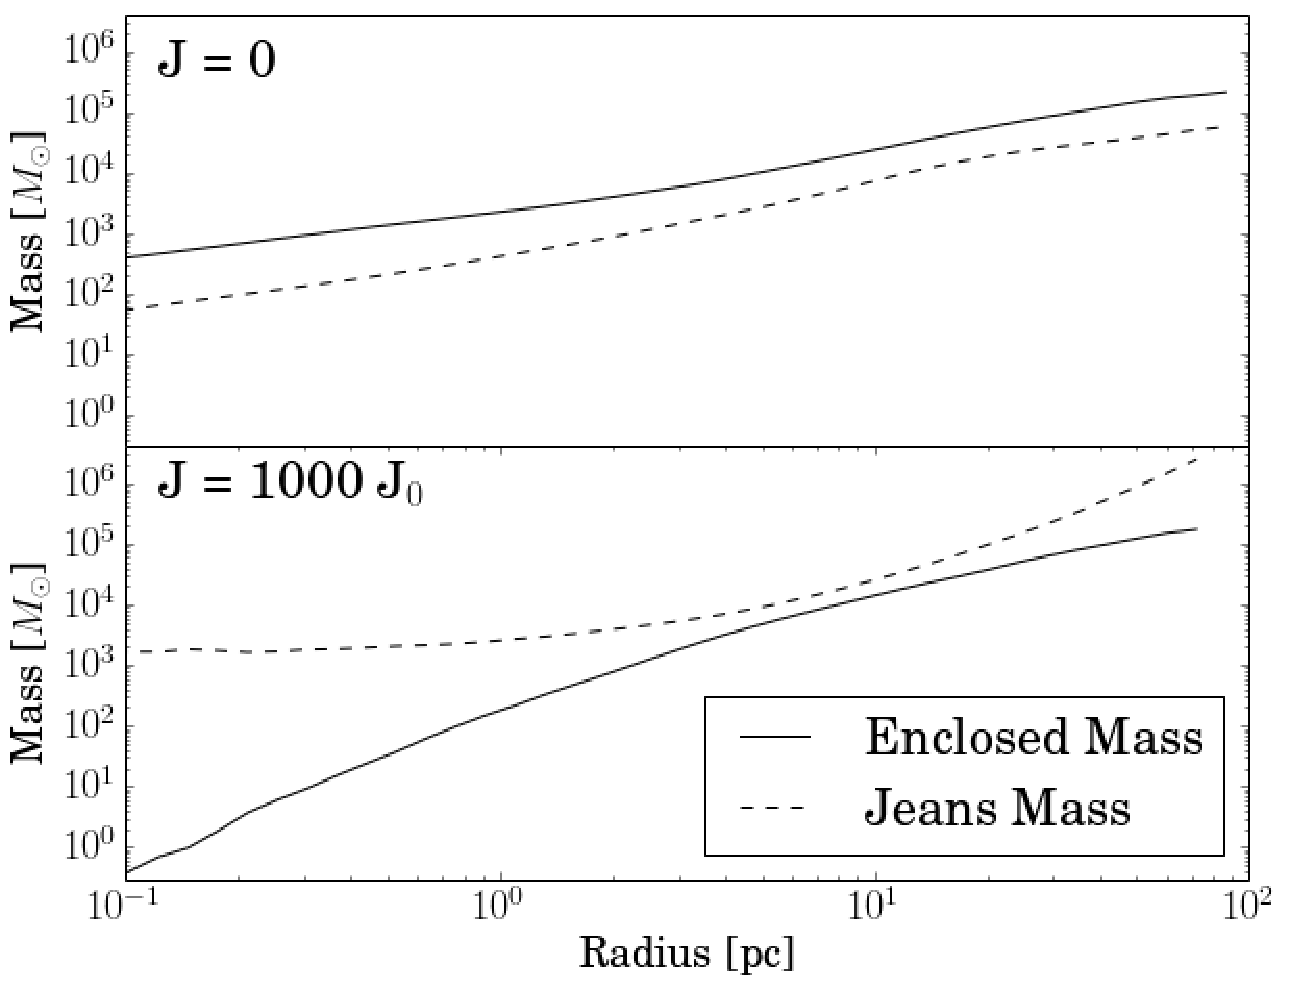
\includegraphics[width=\columnwidth]{figures/halo/blowout}   
    \caption{Shown
      here are the Jeans mass (dotted lines) and total enclosed mass
      (solid lines) within a given radius for  both the $\jxr = 0$ (upper panel) and $\jxr = 1000\,J_0$ case (lower panel). Here we calculate the Jeans mass using the average density and temperature within that radius, extending out to the virial radius of the halo.  The \jxr = 0 case is shown just prior to the formation of the first sink particle; the $\jxr = 1000\,J_0$ case is shown at the maximum density reached over the course of the simulation.}
    \label{suppressed}
  \end{center}
\end{figure}



\begin{figure}
  \begin{center}
    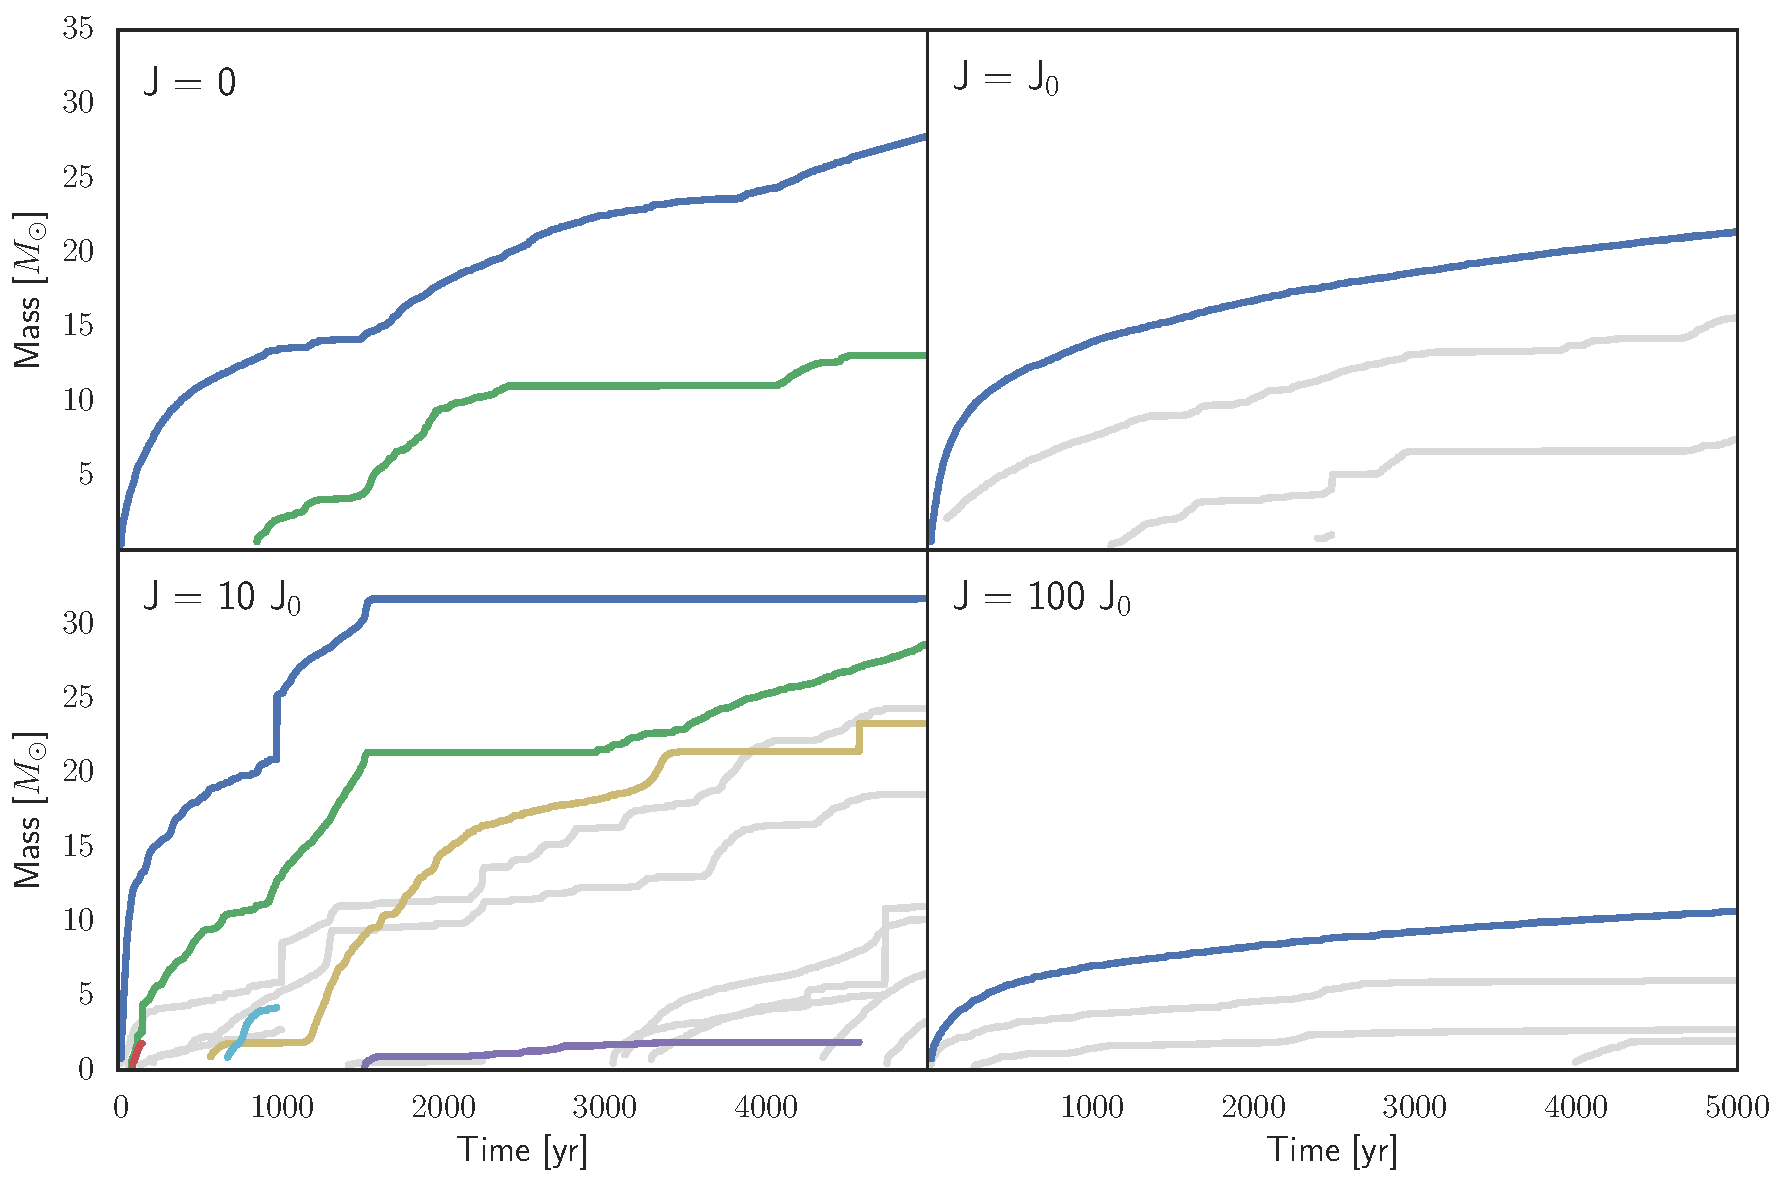
\includegraphics[width=\columnwidth]{figures/sinks/sink_masses}
    \caption{Growth of individual sink particles over time. Sinks for the shielded simulations are coloured throughout in order of formation: blue, green, red, yellow,  cyan, and purple. Lines end where one sink is accreted by another.  The light grey lines show the growth history of sinks in the unshielded simulations for comparison. Note that in the absence of shielding, more sinks form, but the total mass remains roughly constant.}
    \label{sinkmasses}
  \end{center}
\end{figure}

 Once sink formation densities are achieved, there is no clear trend in the subsequent behaviour of the sink particles formed---either in number or accretion rate.  As seen in \RefTab{masstable}, both the virial mass of the minihalo and the cold core mass (defined here as $n\geq10^2\cc$) decrease with increasing \jxr, as expected given the earlier collapse induced by a stronger CXB.  However, at higher densities the $10\,J_0$ case breaks this trend, suggesting that the final stages of the collapse are somewhat chaotic, and influenced more by small-scale randomness related to turbulence than by the strength of the CXB.

 \begin{table}
  \caption{Total gas mass in various minihalo components for each simulation at $t=5000\yr$. Here we have defined $M_{\mathrm core}$ and $M_{\mathrm disc}$ as the total gas mass with $n\geq10^2\cc$ and $n\geq10^8\cc$, respectively. These values are independent of whether shielding is included.}
  \centering
  \begin{tabular}{r c c c c }
    \hline\hline
    \jxr & $M_{\mathrm vir}$ & $M_{\mathrm core}$ & $M_{\mathrm disc}$ & $M_{\mathrm sink}$\\
    & ($10^4\msun$) & ($10^3\msun$) & (\msun) & (\msun) \\
    \hline
    $0$        & 2.4 & 2.5 & 100 & 41 \\
    $J_0$      & 2.2 & 2.2 &  60 & 23 \\
    $10\,J_0$  & 1.9 & 2.1 & 130 & 74 \\
    $100\,J_0$ & 1.2 & 1.3 &  30 & 11 \\
    \hline
    \\
  \end{tabular}
  \label{masstable}
\end{table}

\begin{figure}
  \begin{center}
    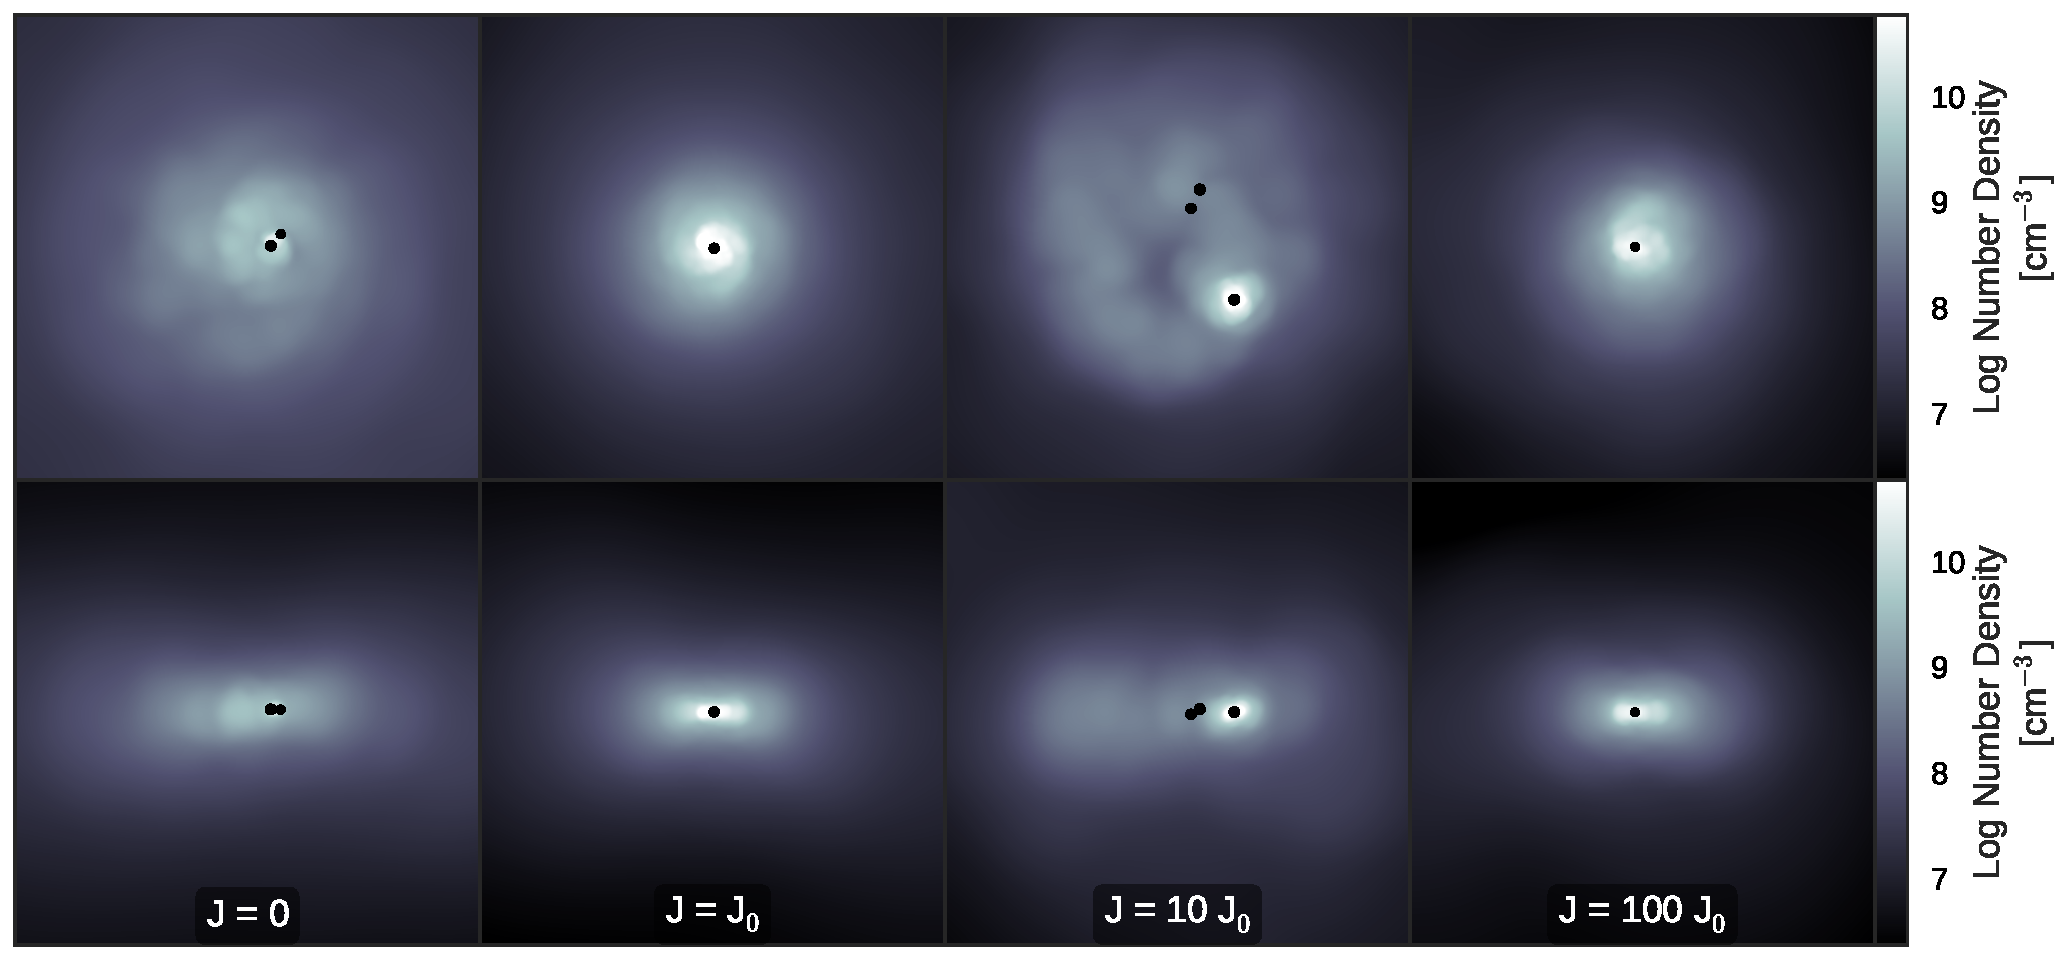
\includegraphics[width=\columnwidth]{figures/structure/disks}
    \caption{Density projection of the central 10000\au of each simulation 5000\yr after formation of the first sink particle. From left to right: $\jxr=0$, $J_0$, $10\,J_0$, $10^2\,J_0$.  Top row shows the face-on density projection; bottom row shows an edge-on projection.  Black dots mark the location of all sink particles, and scale with the mass of the sink.}
    \label{disks}
  \end{center}
\end{figure}

\begin{figure}
  \begin{center}
    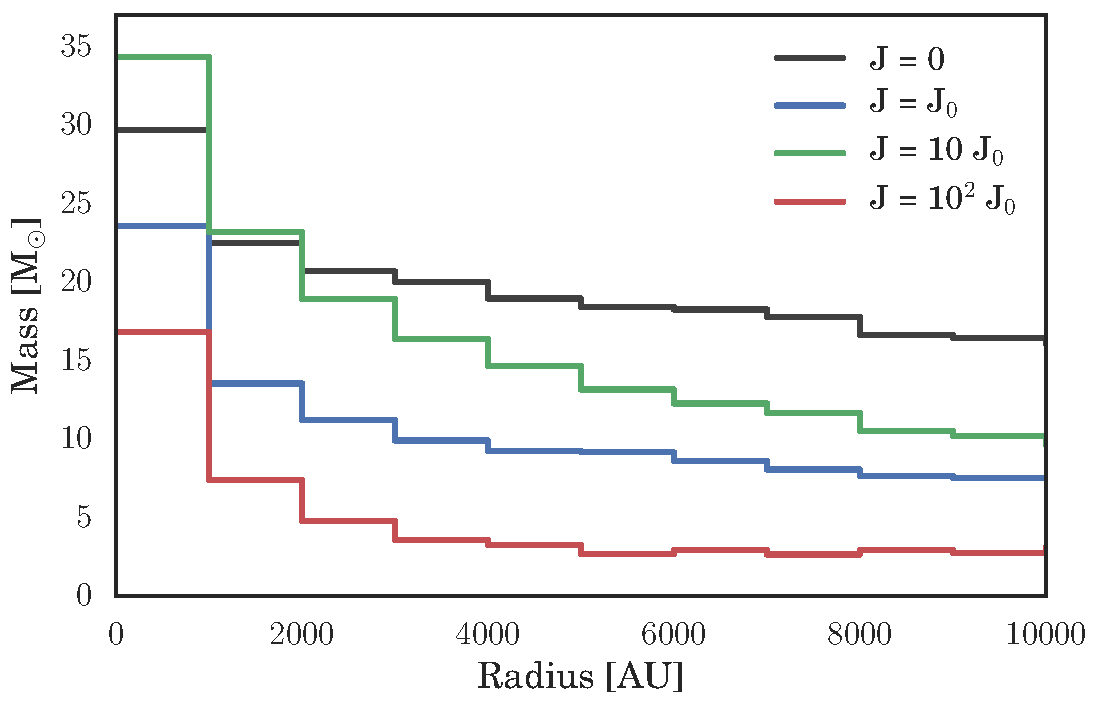
\includegraphics[width=\columnwidth]{figures/radial_bins/mass_bins}
    \caption{Total gas mass in successive radial bins of 500 AU centred on the highest density point in the simulation.  Shown is the mass distribution just prior to the formation of the first sink particle.}
    \label{mbins}
  \end{center}
\end{figure}

\begin{figure}
  \begin{center}
    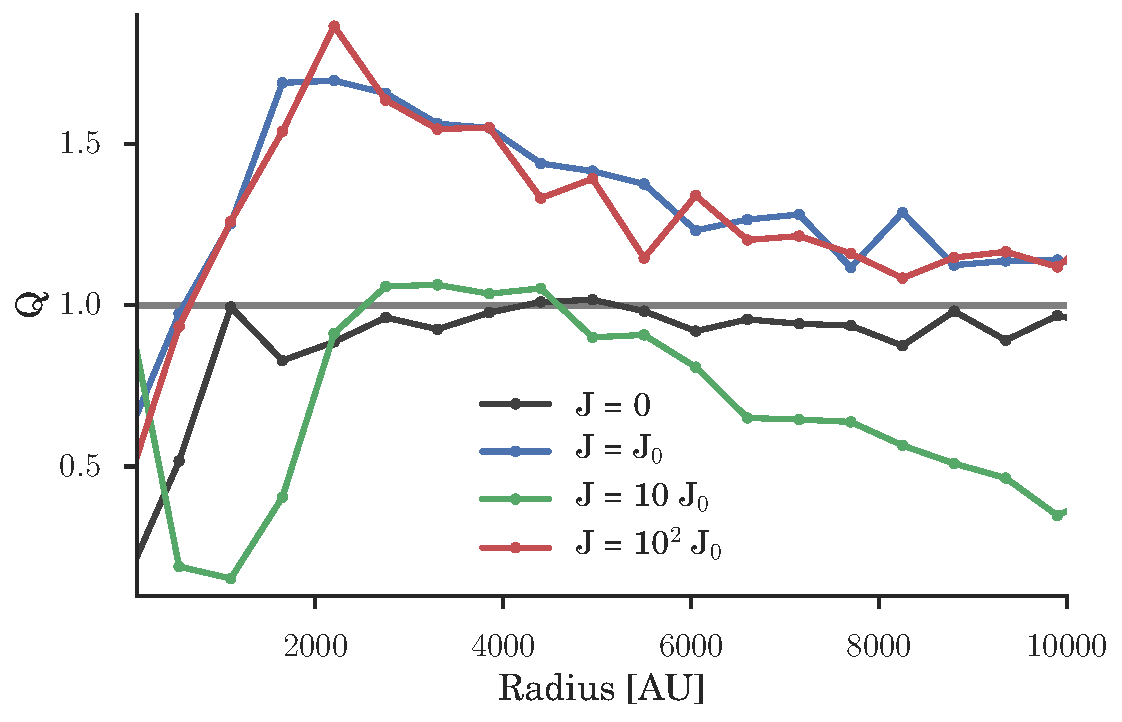
\includegraphics[width=\columnwidth]{figures/radial_bins/toomreQ}
    \caption{The Toomre Q parameter versus radius shown 5000 yr after the first sink particle forms in each simulation.  The accretion disc is susceptible to fragmentation when $Q\lesssim1$, as is the case for the  $\jxr= 0$ and $10\,J_0$ cases.}
    \label{toomreQ}
  \end{center}
\end{figure}


\subsubsection{Disc Fragmentation}
\label{fragmentation}
In the absence of shielding, the gas invariably fragments, forming a binary or small multiple within $1000\yr$.  When shielding is properly accounted for though, excess cooling of the disc ($n\gtrsim10^8\cc$; see \RefFig{Tdens}) is eliminated, and fragmentation is suppressed.  In fact, only a single sink particle forms in both the $\jxr=J_0$ and $100\,J_0$ cases, and while the $10\,J_0$ simulation still fragments, it does so considerably less than in the absence of shielding.  We may quantify this using the Toomre Q parameter \citep{Toomre1964}: 
\begin{equation}
Q = \frac{c_s \kappa}{\pi G \Sigma}
\end{equation}
where $c_s$ is the gas sound speed, $\kappa$ is the epicyclic frequency of the disc, and $\Sigma$ is the surface density; we replace $\kappa$ with the orbital frequency $\Omega$, as appropriate for Keplerian discs.  While the $Q$ parameter specifically applies to infinitely thin isothermal discs, it is correct to within a factor of order unity when applied to thick discs \citep{Wangetal2010}, as is the case here. \RefFig{toomreQ} shows the $Q$ parameter evaluated in mass-weighted spherical shells centred on the accretion disc $5000\yr$ after the first sink particle has formed.  As the mass within these shells is dominated by the disc component, applying this analysis to the disc particles alone would have a negligible impact on the results \citep[e.g.,][]{Greifetal2012}.  The $\jxr=0$ and $10\,J_0$ simulations maintain $Q\lesssim1$ throughout the disc, and are thus susceptible to fragmentation.  On the other hand, save for the central few hundred AU, where they approach the resolution limit of the simulation, the $J_0$ and $100\,J_0$ discs stay well above $Q=1$, hence the lack of fragmentation.

\begin{figure}
  \begin{center}
    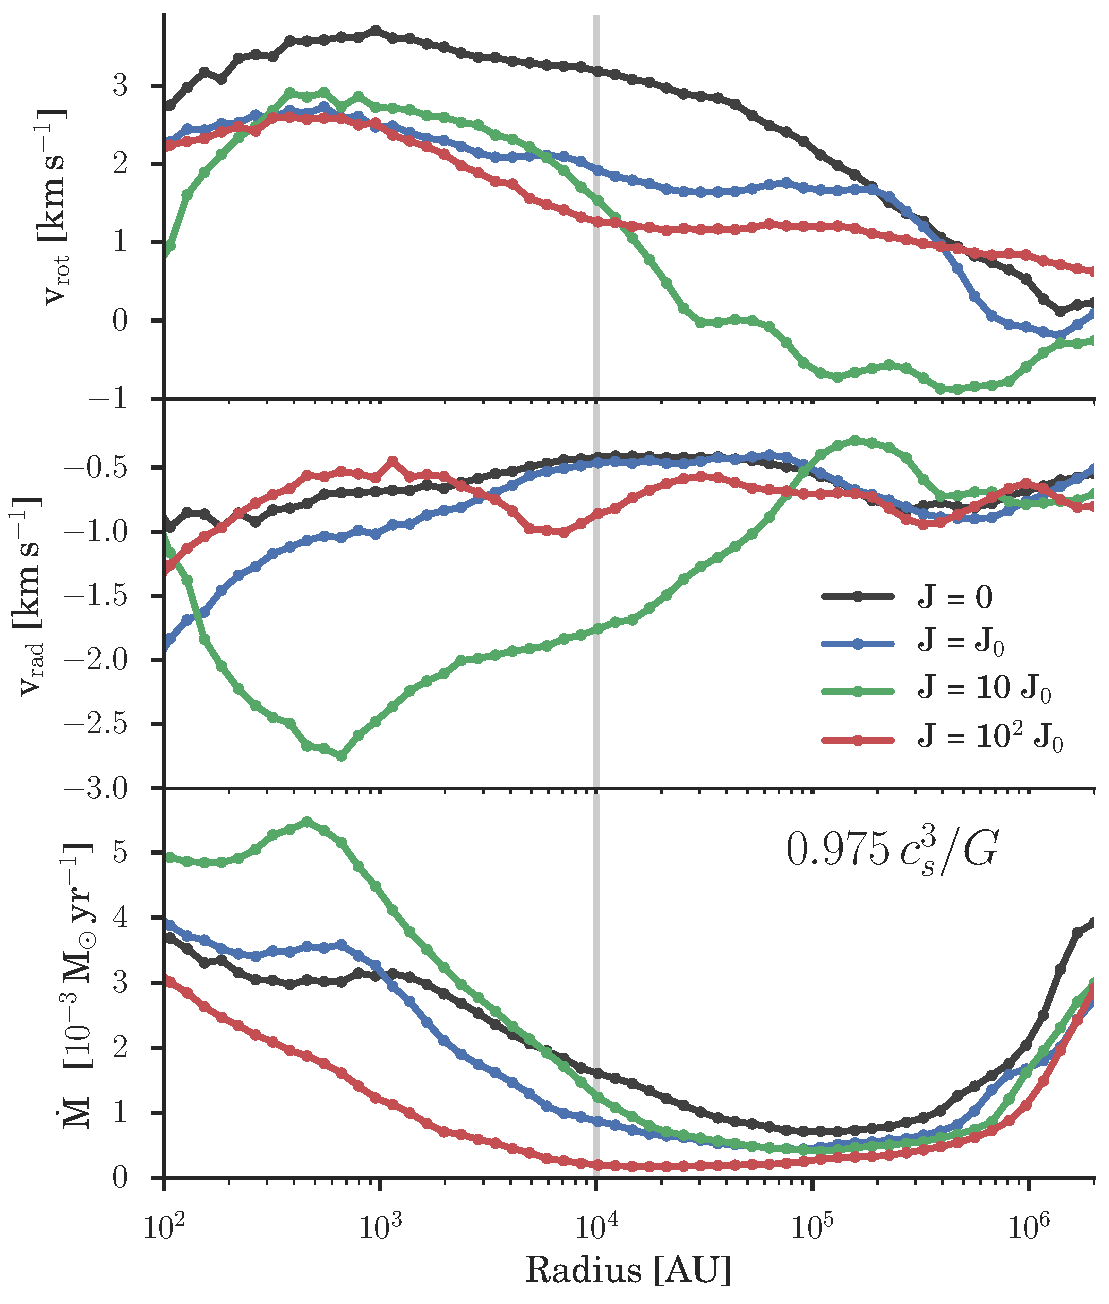
\includegraphics[width=\columnwidth]{figures/radial_bins/core_profile}
    \caption{From top to bottom: the rotational velocity, radial velocity, and Shu accretion rate versus distance to the centre of the minihalo for each simulation as denoted in the legend.  The vertical gray line at $10^4\au$ marks the approximate limit of the accretion disc, and the limit to which Figures \ref{disks}, \ref{mbins} and \ref{toomreQ} are displayed.  Note the significant discrepancies in the behaviour of the $\jxr=10\,J_0$ case in each panel.}
    \label{core_profile}
  \end{center}
\end{figure}
While the $\jxr=10\,J_0$ minihalo also collapses early, in the same manner as the $J_0$ and $100\,J_0$ simulations, it still experiences significant fragmentation.  This is primarily due to the specific details of its collapse history, modulated by small-scale turbulence, rather than the precise value of \jxr, and can be understood by examining the velocity profile of the minihalo, shown in \RefFig{core_profile} along with the Shu accretion rate \citep{Shu1977} for mass-weighted spherical bins out to $\sim$$10\pc$. While the inner regions of the $10\,J_0$ accretion disc exhibit approximately Keplerian rotation in line with the other simulations, the gas at large radii experiences significantly less rotational support.  This results in a much larger infall velocity, leading in turn to a higher accretion rate.  This overwhelms the ability of the accretion disc to support itself against the growth of perturbations, resulting in significant fragmentation.


%==============================================================================
\section{Summary and Conclusions}
\label{conclusions}
We have performed a suite of cosmological simulations employing a range of CXB models, focusing on the impact of such a background on Pop III stars forming in a minihalo.  As three-body processes turn the gas fully molecular by $n=10^{12}\cc$, following the evolution of the gas up to this density allows us to fully capture the impact of a CXB on \htwo and \hd cooling in the gas.  After the gas reaches $10^{12}\cc$ we form sink particles, enabling us to study the subsequent evolution of the system, which we follow for an additional 5000\yr.

X-rays have two competing effects on primordial gas, as ionising the gas serves to both heat it and increase the number of free electrons, which catalyse the formation of molecular hydrogen.  As \htwo is the main coolant in primordial gas, this actually enhances cooling.  We find that heating dominates in low density gas, but is overwhelmed at higher densities by the enhanced cooling X-rays provide.  The transition between these two regimes occurs between $n=1$ and 100\cc, depending on the strength of the CXB.  

Previous work investigating the impact of a CXB on structure formation in the early universe has generally been found to increase the supply of cold gas in a given halo \citep{HaimanAbelRees2000, VenkatesanGirouxShull2001, GloverBrand2003, Cen2003, KuhlenMadau2005, Jeonetal2012}.  In particular, \citet{KuhlenMadau2005} found the increase in cold gas available for star formation was greatest in $2\times10^5$--$10^6\msun$ minihaloes, where the increase could exceed 1--2 orders of magnitude for moderate X-ray ionisation rates. This comports with our findings---allowing the X-ray irradiated haloes to evolve to the same cosmic time as the $\jxr=0$ minihalo would result in a relatively larger supply of cold dense gas. As X-rays penetrating the minihalo begin to experience significant attenuation above $n\sim10^6\cc$ though, the primary impact of a CXB is on gas in the loitering phase and below. While X-ray heating dominates below $n\sim 1\cc$, minihaloes that overcome this impediment collapse earlier, as the cooler gas in the loitering phase requires a smaller Jeans mass to proceed to high densities.  

The X-ray background is severely attenuated by the time it reaches sink formation densities. As a result its impact on the gas temperature is largely neutral, with the subsequent behaviour of the sink particles formed influenced more by small-scale  turbulence than the strength of the CXB.  Consequently, the characteristic mass of the stars formed is quite stable even as we vary the CXB strength by several orders of magnitude, and does not change dramatically even when the supply of cold gas in the centre of the minihalo is significantly increased, as in the $10\,J_0$ case.  Instead, this causes the disc to fragment, forming several protostellar cores.

It should be noted that these findings are somewhat sensitive to the density at which the minihalo becomes opaque to X-rays.  While we found no difference in the total column density between simulations, a more robust estimate of the local column density would be beneficial \citep[e.g.,][]{Hartwigetal2015, Safranek-Shraderetal2012}. Additionally, there is a possibility that the more rapid minihalo collapse induced by a strong CXB may have an impact on the velocity dispersion of the infalling gas, suppressing fragmentation and possibly increasing the mass of the stars formed. While our simulations lack sufficient resolution to verify this, the findings of \citet{Clarketal2011a} suggest that stars forming in pre-ionised minihaloes experience more turbulence, resulting in a somewhat larger characteristic mass than in pristine minihaloes. Finally, our findings may have implications for reionisation and the 21-cm signal \citep{FurlanettoPengBriggs2006, Mirocha2014}: while the impact on the number of fragments and characteristic mass of Pop III appears to be nearly neutral, low-density gas is still smoothed by X-ray heating, thus resulting in a lower IGM clumping factor.


\chapter{Population III Star Formation Under Cosmic Ray Feedback}
\section{Introduction}
\label{intro}

Cosmic rays (CRs) have long been known to play an important role in the complex physics and chemistry of the interstellar medium (ISM) in local galaxies (\citealt{SpitzerTomasko1968,SpitzerScott1969,GlassgoldLanger1973,GoldsmithLanger1978,CravensDalgarno1978,MannheimSchlickeiser1994,Tielens2005}; recently reviewed by \citealt{StrongMoskalenkoPtuskin2007,GrenierBlackStrong2015}).  
They are an effective source of ionisation and heating in various environments, from preheating the primordial intergalactic medium  \citep[IGM;][]{SazonovSunyaev2015}, to driving outflows in the diffuse ISM \citep[e.g.,][]{Ensslinetal2007,Jubelgasetal2008,SalemBryan2014,Hanaszetal2013,Boothetal2013,SalemBryanHummels2014}, to providing an important (often dominant) source of heating and ionisation in deeply embedded gas clouds and protostellar discs \citep{Spitzer1978,DalgarnoYanLiu1999,IndrioloFieldsMcCall2009,PadovaniGalliGlassgold2009,GlassgoldGalliPadovani2012,PadovaniHennebelleGalli2013,Padovanietal2015}. 

CRs are particularly interesting in the context of Population III (Pop III) star formation, as they provide a continually replenished source of free electrons, enhancing the formation of molecular hydrogen---the only coolant available in primordial gas \citep{Abeletal1997,GalliPalla1998,BrommCoppiLarson2002}.  
This enhances the ability of the gas to cool, modifying the characteristic density and temperature at which runaway gravitational collapse sets in, and possibly the characteristic mass of the stars thus formed.   
The characteristic mass of Pop III is critical, as it largely controls the extent to which the first stars influence their environment, determining both their total luminosity and ionising radiation output \citep{Schaerer2002}, in addition to the details of their eventual demise \citep{Hegeretal2003,HegerWoosley2010,MaederMeynet2012}. 
As such, a thorough understanding of how the very first stars impact subsequent episodes of metal-free star formation---sometimes referred to as Pop III.1 and Pop III.2, respectively \citep{McKeeTan2008}---is crucial to developing a comprehensive picture of cosmic evolution.

In the absence of any feedback, pioneering numerical studies suggested that the very first stars were quite massive---on the order of $100\msun$ \citep[e.g.,][]{BrommCoppiLarson1999,BrommCoppiLarson2002,AbelBryanNorman2002,Yoshidaetal2003,BrommLarson2004,Yoshidaetal2006,OSheaNorman2007}. 
However, more recent simulations, aided by increased resolution, have found that significant fragmentation occurs during the star formation process \citep{StacyGreifBromm2010,Clarketal2011a,Clarketal2011b,Greifetal2011,Greifetal2012,StacyBromm2013,Hiranoetal2014,Hosokawaetal2015}, leading to the emerging consensus that the Pop III initial mass function (IMF) was somewhat top-heavy with a characteristic mass of $\sim$ a few $\times 10\msun$ \citep{Bromm2013}. 
While the contribution these stars make to chemical enrichment (\citealt{MadauFerraraRees2001,MoriFerraraMadau2002,BrommYoshidaHernquist2003,Hegeretal2003,UmedaNomoto2003,TornatoreFerraraSchneider2007,Greifetal2007,Greifetal2010,WiseAbel2008,Maioetal2011}; recently reviewed in \citealt{KarlssonBrommHawthorn2013}) and  reionisation \citep{Kitayamaetal2004,Sokasianetal2004,WhalenAbelNorman2004,AlvarezBrommShapiro2006,JohnsonGreifBromm2007,Robertsonetal2010} have been well studied, the consequences for Pop III stars forming in neighbouring minihaloes have been less thoroughly explored.  

As Pop III stars form in a predominantly neutral medium, the majority of their ionising output is absorbed, allowing only radiation less energetic than the Lyman-$\alpha$ transition to escape the immediate vicinity of the star-forming halo.  
While far-ultraviolet radiation in the Lyman-Werner (LW) bands ($11.2 - 13.6\ev$) lacks sufficient energy to interact with atomic hydrogen, it can still effectively dissociate molecular hydrogen.  
However, studies have found that the expected mean value of such radiation is far below the critical LW flux required to suppress $\htwo$ cooling \mbox{\citep{Dijkstraetal2008}}. 
At the high energy end, the neutral hydrogen cross section for X-rays and cosmic rays is small, allowing them to easily escape their host minihaloes. 
We recently investigated the impact of a cosmic X-ray background generated by high-mass X-ray binaries on primordial star formation \citep{Hummeletal2015}; here we focus on the impact of a CR background consisting of particles accelerated in supernova shock waves via the first-order Fermi process (see Section \ref{sec:context}).  

While the uncertainties involved in estimating the strength of the high-$z$  CR background are huge,  measurements of the $^6{\mathrm Li}$ abundance from metal-poor stars in the Galactic halo provide a useful constraint: the observed abundance of  $^6{\mathrm Li}$ is approximately 1000 times higher than predicted by big bang nucleosynthesis \citep{Asplundetal2006}, strong evidence for the existence of a CR spallation channel to provide a $^6{\mathrm Li}$ bedrock abundance prior to the bulk of star formation \citep{RollindeVangioniOlive2005,RollindeVangioniOlive2006}. 
Production of this first pervasive CR background by shock-acceleration in Pop III supernovae dovetails nicely with the upper limits this places on the CR energy density at high redshifts \citep{RollindeVangioniOlive2006}.

Early studies of the impact of CRs on primordial star formation focused on the production of ultra-high-energy CRs (UHECRs) by the decay of ultra-heavy X particles \citep{ShchekinovVasiliev2004,VasilievShchekinov2006,RipamontiMapelliFerrara2007}.  
With energies above the Greisen--Zatsepin--Kuzmin (GZK) cutoff \citep{Greisen1966,ZatsepinKuzmin1966}, UHECRs interact with the cosmic microwave background (CMB) to produce ionising photons, which in turn enhance the free electron fraction of the gas.  
Other work investigated the direct collisional ionisation of neutral hydrogen by SN shock-generated CRs, using one-zone models to determine the impact of a CR background on the chemical and thermal evolution of the gas in a minihalo \citep{StacyBromm2007,JascheCiardiEnsslin2007}.  
These studies found that the presence of a CR background enhanced molecular hydrogen formation in the minihalo, cooling the gas and lowering the Jeans mass, and by extension, the characteristic mass of the stars formed. 
We expand upon these one-zone models, using three-dimensional \textit{ab initio} cosmological simulations to investigate the impact of a CR background on Pop III stars forming in a minihalo.

This paper is organized as follows: In Section \ref{sec:context} we provide the cosmological context for this study, estimating the expected intensity of the CR background. Our numerical methodology is described in Section \ref{sec:methods}, while our results are presented in Section \ref{sec:results}.  
Finally, our conclusions are gathered in Section \ref{conclusions}. Throughout this paper we adopt a $\Lambda$CDM model of hierarchical structure formation, using the following cosmological parameters, consistent with the latest measurements from the Planck Collaboration \citep{PlanckParams2015}: $\Omega_{\Lambda} = 0.7$, $\Omega_{\mathrm m} = 0.3$, $\Omega_{\mathrm B} = 0.04$, and $H_0 = 70 \kms \Mpc^{-1}$.

\section{Cosmic Rays in the Early Universe}
\label{sec:context}
While there are several possible sources of CRs at high redshifts including primordial black holes, topological defects, supermassive particles, and structure formation shocks, the most likely source in the early Universe is supernova (SN) explosions \citep[e.g.,][]{GinzburgSyrovatskii1969,BiermannSigl2001,Stanev2004,Pfrommeretal2006}, wherein CRs are accelerated by the SN shock wave via the first-order Fermi process \citep[e.g.,][]{Bell1978}.  
In this scenario, high-energy particles diffuse back and forth across the shock front, increasing their energy by a small percentage each time, and resulting in a differential spectrum of CR number density per energy \citep{Longair1994} of the form
\begin{equation}
    \frac{{\mathrm d}n_{\mathrm \small CR}}{{\mathrm d}\epsilon} = \frac{n_{\mathrm norm}}{\epsilon_{\mathrm min}}
    \left( \frac{\epsilon}{\epsilon_{\mathrm min}} \right)^{-2},
\end{equation}
where $n_{\mathrm \small CR}$ is the CR number density, $\epsilon$ is the kinetic energy of the CR, $\epsilon_{\mathrm min}$ is the low-energy cutoff of the CR spectrum, and $n_{\mathrm norm}$ is a normalising density factor. 

The value of $\epsilon_{\mathrm min}$ is crucial, as the ionisation cross-section of non-relativistic CRs varies roughly as $\epsilon^{-1}$ for $\epsilon \gtrsim 10^5\ev$. 
Higher energy CRs thus travel much farther between interactions and are less able to effectively deposit their energy into the gas, such that the low-energy end of the CR spectrum provides the majority of the ionisation and heating.  
While estimates of the lowest possible energy CR protons could gain in a SN shock wave vary significantly, below $10^5\ev$ the velocity of the CR drops below the approximate orbital velocity of electrons in the ground state of atomic hydrogen, and the interaction cross-section diminishes rapidly \citep{Schlickeiser2002}. 

We therefore employ $\epsilon_{\mathrm min} = 10^6\ev$ as the lower bound for the CR background in our simulations.  
While CRs with energies below $10^6\ev$ may account for $\sim$$5-50$ percent of the CR energy budget, they also deposit a substantial fraction of their energy into the IGM \citep{SazonovSunyaev2015}. 
Consequently, they are unable to efficiently contribute to the build-up of a large-scale CR background. We thus neglect the contribution such CRs make to the ionisation and heating of primordial gas. 
However, this introduces only minor errors, as shown by \citet{StacyBromm2007}. Using one-zone models, they found that extending the CR spectrum to as low as $\epsilon_{\mathrm min} = 10^3\ev$ altered the resulting ionisation and heating rates by less than a factor of two.  
It should also be noted that the uncertainty in $\epsilon_{\mathrm min}$ is on par with that for the fraction of the SN energy going into CR production, $f_{\mathrm \small CR}$, which is expected to be $\sim$$10-20$ percent \citep{CaprioliSpitkovsky2014}.  
Here we assume $f_{\mathrm \small CR} = 0.1$.

The upper limit of the CR energy spectrum $\epsilon_{\mathrm max}$ depends on the strength of the ambient magnetic field in the local ISM, as the Fermi acceleration process is linearly dependent on the magnetic field through which the SN shock wave propagates. 
As the strength, generation mechanism, and distribution of magnetic fields in the early Universe remain highly uncertain \citep{DurrerNeronov2013}, we set $\epsilon_{\mathrm max} = 10^{15}\ev$, a typical maximum value from Fermi acceleration theory in SN shocks \citep[e.g.,][]{BlandfordEichler1987}.  
So long as $\epsilon_{\mathrm max}$ is below the GZK cutoff, $\epsilon_{\mathrm \small GZK}$, at that redshift, given by \citep{StacyBromm2007}
\begin{equation}
\epsilon_{\mathrm \small GZK}(z) = \frac{5\times10^{19}\ev}{1+z},
\end{equation}
the precise value of $\epsilon_{\mathrm max}$ is not crucial, since the great majority of the heating and ionisation is provided by CRs near $\epsilon_{\mathrm min}$.

Magnetic fields also play an important role in isotropising the CR background.  
We may estimate the effective mean free path over which a CR can freely propagate before being significantly impacted by the presence of a magnetic field $B$ using the Larmor radius $r_L$, where for a proton, 
\begin{equation}
r_L = \frac{\gamma \mh \beta c^2}{eB}.
\end{equation}
Here, $\gamma$ is the Lorentz factor of the CR; $\mh$, the proton mass; $e$, the proton charge; $c$, the speed of light, and $\beta c$ is the CR velocity. 
The CR background at redshift $z$ for protons with energy $\epsilon$ may then be considered fully isotropic if $r_L(\epsilon) \ll \Dhubble(z)$ where $\Dhubble(z)$ is the Hubble distance at that epoch. 
Recent observations have placed lower bounds on the modern-day intergalactic magnetic field strength ranging from $10^{-18}\,$G \citep{Dermeretal2011} to $3\times10^{-16}\,$G \citep{NeronovVovk2010}, while other estimates place the field strength as high as $10^{-15}\,$G \citep{AndoKusenko2010}.  
Simply accounting for flux freezing, the magnetic field at redshift $z$ is given by
\begin{equation}
B(z) = B_0 (1+z)^2,
\end{equation}
where $B_0$ is the magnetic field at the current epoch. 
The magnetic field strength in the IGM at $z=20$ then was likely in the range $4\times10^{-16}$ to $4\times10^{-13}\,$G.  
The magnetic field strength required to fully randomize the path of a $10^{15}\ev$ CR proton is $\sim$$10^{-14}\,$G; we may therefore assume the CR background is fully isotropic to the limit of our CR spectrum.  
The Larmor radius for a $10^6\ev$ CR proton in a $10^{-15}\,$G magnetic field, on the other hand, is $\sim$$10\pc$.  
While unable to freely propagate, under the assumption that magnetic fields at these redshifts are disordered on $\pc$ scales, such CRs will diffuse through the IGM with a diffusion coefficient $D = c r_{\mathrm L}$.  
Given that the typical physical distance $L$ between minihaloes at $z=20$---derived from the Press-Schechter (\citeyear{PressSchechter1974}) formalism---is $\sim$$5\kpc$, the diffusion time between minihaloes, $t_{\mathrm diff} = L^2/D$, is of order $10^{14}\s$, less than the Hubble time at this epoch.
$10^6\ev$ CRs are thus able to build up a locally isotropic background on scales larger than the typical distance between minihaloes.
On the scale of our simulation boxes (see Section \ref{setup}), CRs are thus able to build up an effectively uniform and isotropic background from $10^6$ to $10^{15}\ev$, an assumption we make throughout the remainder of our analysis.

Normalising the differential CR spectrum with the aforementioned limits $\epsilon_{\mathrm min}$ and $\epsilon_{\mathrm max}$ to the total energy density in cosmic rays, $\ucr$, results in a CR energy spectrum increasing over cosmic time in the following fashion:
 \begin{equation}
 \frac{{\mathrm d}n_{\mathrm \small CR}}{{\mathrm d}\epsilon}(z) = \frac{u_{\mathrm \small CR}(z)}{\epsilon_{\mathrm min}^2{\mathrm ln}\,\epsilon_{\mathrm max}{\large /}\epsilon_{\mathrm min}}  \left( \frac{\epsilon}{\epsilon_{\mathrm min}} \right)^{-2}.
 \end{equation}
Here we estimate $\ucr$ as follows:
\begin{equation}
u_{\mathrm \small CR}(z) = f_{\mathrm \small CR} E_{\mathrm \small SN}\, f_{\mathrm \small SN} \Psi_{*}(z)\, t_{\mathrm \small H}(z) (1+z)^3,
\end{equation}
where $f_{\mathrm \small CR}$ is the fraction of the SN explosion energy $E_{\mathrm \small SN}$ going into CR production, $f_{\mathrm \small SN}$ is the mass fraction of stars formed which die as SNe, and $\Psi_{*}(z)$ is the comoving star formation rate density (SFRD) as a function of redshift, which we assume to be constant over a Hubble time $t_{\mathrm \small H}$. 
The factor of $(1+z)^3$ accounts for the conversion from a comoving SFRD to a physical energy density. As in \citet{Hummeletal2015}, we base our estimate of $u_{\mathrm \small CR}(z)$ on the Pop III SFRD calculated by \citet{GreifBromm2006}, but see \citet{Campisietal2011} for a more recent calculation. 

The mass fraction of Pop III stars dying as SNe depends strongly on their IMF, and while the complex physical processes at play in gas collapsing from IGM to protostellar densities have so far prevented a definitive answer to this question, the emerging consensus is that the Pop III IMF was somewhat top-heavy with a characteristic mass of $\sim$ a few $\times 10\msun$ \citep{Bromm2013}.  
Given this, we assume one SN is produced for every $50\msun$ of stars formed and each SN-producing star dies quickly as a core-collapse explosion with $E_{\mathrm \small SN} = 10^{51}\erg$, 10 percent of which goes into CR production.  

This fiducial estimate for $\ucrz$---henceforth referred to as model $u_0$---is shown in Figure \ref{fig:ucr}, where we compare the energy density in CRs to the gas thermal energy density in the IGM, the range of estimates for the IGM magnetic field energy density, and the energy density of the cosmic microwave background. 
We also mark the most conservative upper limits placed on $\ucr$ by \citet{RollindeVangioniOlive2006}, calculated using the observed overabundance of $^6$Li compared to big bang nucleosynthesis. 
Given the huge uncertainties inherent in estimating the strength of the high-$z$ CR background, we also consider five additional models with 10, $10^2$, $10^3$, $10^4$, and $10^5$ times the energy density of model $u_0$, as shown in Figure \ref{fig:ucr}.  
This allows us to bracket the plausible range of energy densities, from values comparable to the IGM thermal energy density to just below the upper limits from $^6$Li abundance measurements.
 

\begin{figure}
\begin{center}
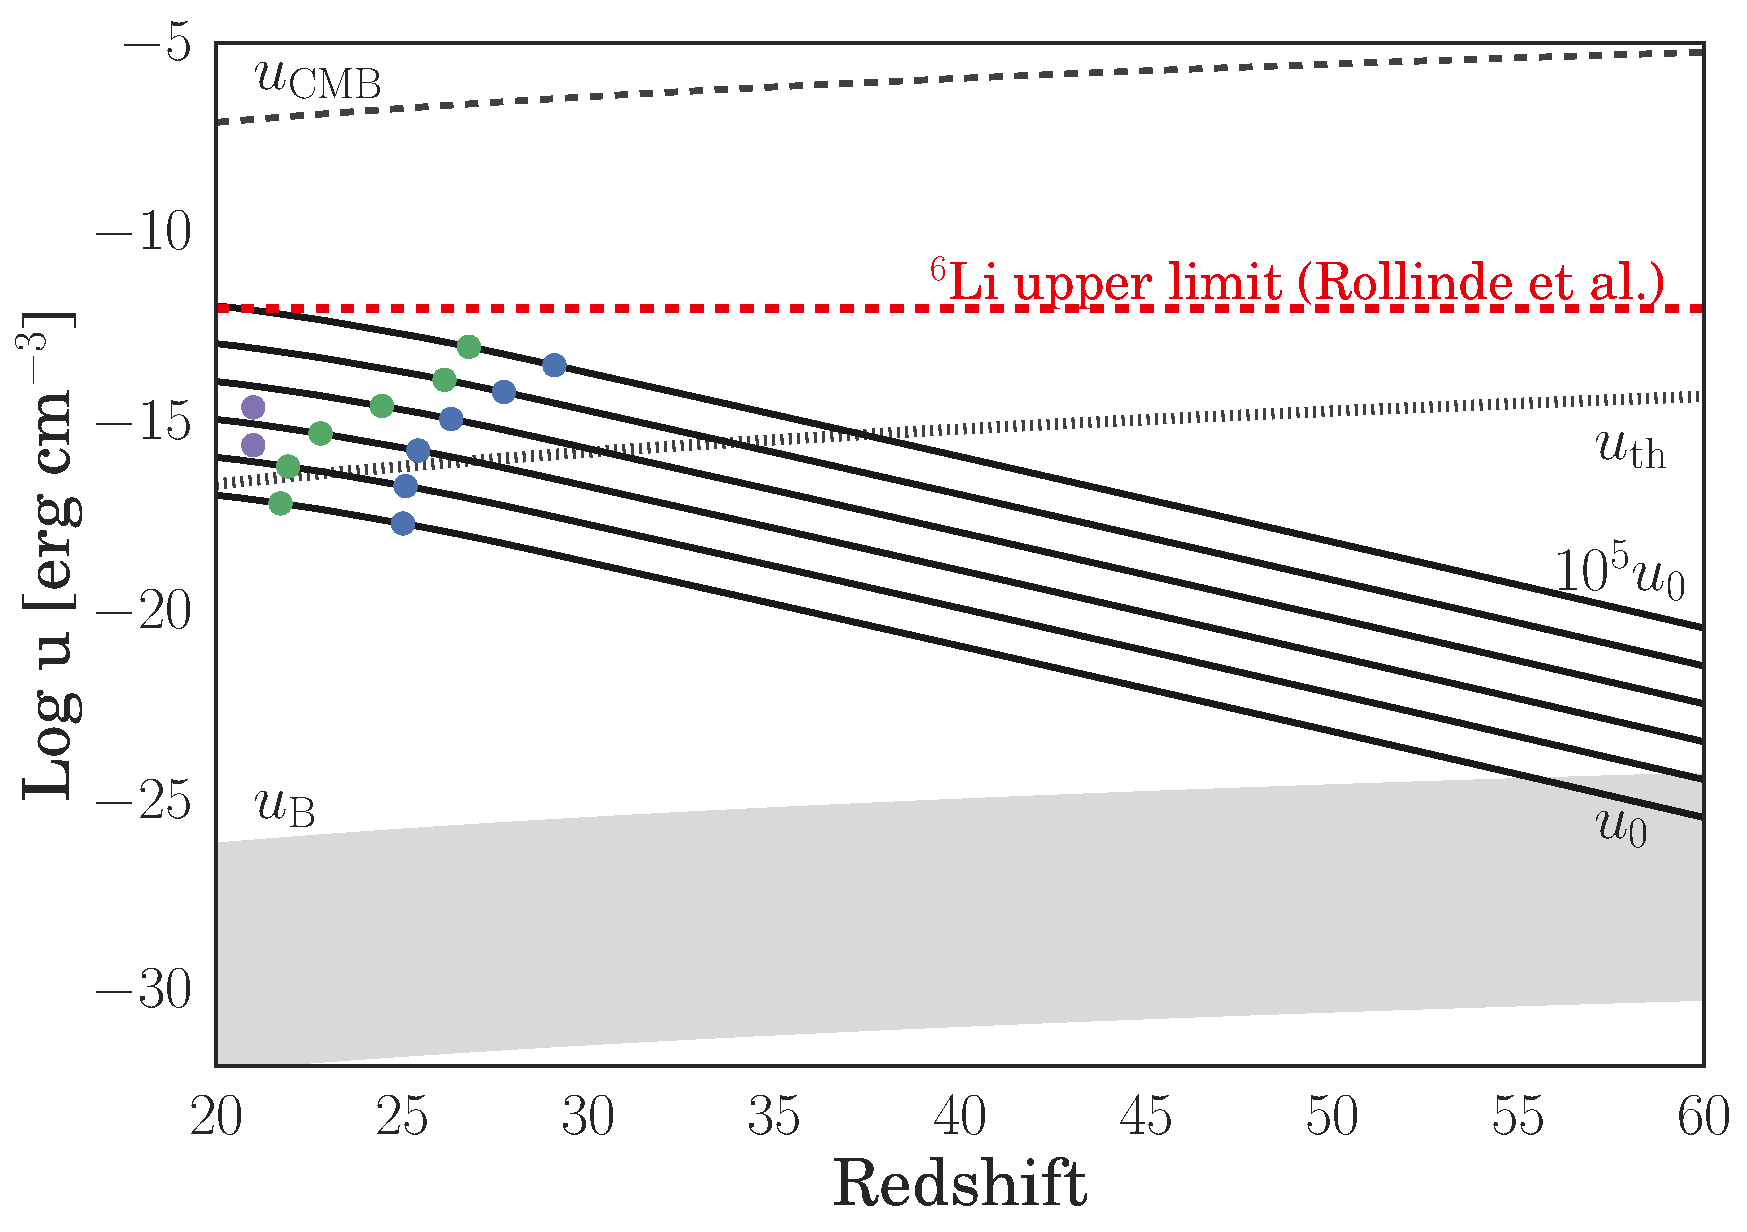
\includegraphics[width=1\columnwidth]{figures/u_cr/u_cr}
\caption{\label{fig:ucr}
Cosmic ray energy density $\ucr$ as a function of redshift.  
Our models, from $u_0$ to $10^5u_0$ are indicated by solid black lines, while the energy density in the CMB and the thermal energy density in the IGM are denoted by dashed and dotted black lines, respectively. 
The grey region shows the range of possible values for the magnetic field energy density in the IGM, and the dashed red line marks the most conservative upper limit on the CR energy density from \citet{RollindeVangioniOlive2006}, as derived from the $^6$Li abundance. 
Blue points indicate the redshift at which Halo 1 collapses to high densities for a given $\ucr$; green points, the redshift at which Halo 2 collapses.  
Finally, purple points denote the energy densities employed by \citet{StacyBromm2007} to study the impact of a CR background using one-zone models calculated at $z=21$.%
}
\end{center}
\end{figure}

\section{Numerical Methodology}
\label{sec:methods}
Using the well-tested $N$-body smoothed particle hydrodynamics (SPH) code GADGET-2 \citep{Springel2005}, we perform our simulations using the same chemistry network and sink particle method as described in \citet{Hummeletal2015}; the relevant details are summarized below.  
In addition to using the same initial conditions as in \citet{Hummeletal2015} to allow for a comparison of the impact of X-rays versus cosmic rays on the primordial gas, we perform a second suite of simulations using new initial conditions.  
The minihalo in these simulations collapses at a lower redshift; this allows us to ensure our results are not being influenced by the CMB temperature floor.

\subsection{Initial Setup}
\label{setup}
The first set of simulations (henceforth referred to as Halo 1) use the same initial conditions as \citet{Hummeletal2015} and \citet{StacyGreifBromm2010}, and are initialised at $z=100$ in a 140 comoving kpc box with periodic boundary conditions. 
To accelerate structure formation within the simulation box an artificially enhanced normalisation of the power spectrum, $\sigma_8 = 1.4$, was used, but the simulations are otherwise initialised in accordance with a $\Lambda$CDM model of hierarchical structure formation. 
For a discussion of the validity of this choice, see \citet{StacyGreifBromm2010}. 
High resolution in these simulations is achieved using a standard hierarchical zoom-in technique, with nested levels of refinement at 40, 30, and 20 kpc (comoving).  
Using this technique, the highest resolution SPH particles have a mass $m_{\mathrm SPH} = 0.015\msun$, yielding a minimum mass resolution $M_{\mathrm res} \simeq 1.5 N_{\mathrm neigh} m_{\mathrm SPH} \lesssim 1\msun$ for the simulation.  
Here $N_{\mathrm neigh} = 32$ is the number of particles used in the SPH smoothing kernel \citep{BateBurkert1997}.

The initial conditions for the second set of simulations (henceforth referred to as Halo 2) are derived from the simulations described in \citet{StacyBromm2013}.  
These simulations were initialised at $z=100$ in a 1.4 comoving Mpc box in accordance with the same $\Lambda$CDM structure formation model as Halo 1, but with $\sigma_8 = 0.9$ rather than the artificially enhanced $\sigma_8 = 1.4$ used in Halo 1. 
The use of `marker sinks'  for regions reaching densities beyond $n=10^3\,{\mathrm cm}^{-3}$ rather than following the gas to higher densities allows for the efficient identification of the first 10 minihaloes to form within the box; we select the final minihalo to form---i.e., Minihalo 10 from \citet{StacyBromm2013}---for further study.  
After identifying the location of the final minihalo, the cosmological box is re-initialised at $z=100$ using a standard zoom-in technique with two nested levels of refinement used to improve resolution surrounding the selected minihalo.  
Each `parent' particle within the most refined region is split into 64 `child' particles, with a minimum mass of $m_{\mathrm gas}=1.85\msun$ and $m_{\mathrm \small DM}=12\msun$. 
These refined simulations are then run until the gas approaches the typical onset of runaway collapse at $n=10^4\cc$.

\subsubsection{Halo 2 Cut-out and Refinement}
\label{cutout}

Once the simulation reaches $10^4\cc$ all particles beyond 10 comoving kpc from the centre of the collapsing minihalo are removed to conserve computational resources. 
To achieve a maximum resolution comparable to Halo 1, all particles within the 10 comoving kpc volume are split into two child particles placed randomly within the smoothing kernel of the parent particle.  
This particle-splitting is repeated twice more; all particles within 8 comoving kpc are replaced by 8 child particles; within 6 comoving kpc, each of these child particles is split into an additional 8 for a total of 128 child particles in the most refined region.  
At each step, the mass of the parent particle is evenly divided among the child particles and the smoothing length is set to $h N_{\mathrm new}^{-1/3}$, where $h$ is the smoothing length of the parent and $N_{\mathrm new}$ is the number of child particles created.  
All particles inherit the same entropy, velocity, and chemical abundances as their parent, ensuring conservation of mass, internal energy, and momentum.

While our cut-out technique leads to a rarefaction wave propagating inward from the suddenly introduced vacuum boundary condition, the average sound speed at the edge of the most refined region is $\sim$$1\,{\mathrm km}\,{\mathrm s}^{-1}$.  
As a result the wave only travels $\sim$$0.5\,$pc over the remaining 400,000$\,$yr of the simulation, a negligible fraction of the $\sim$350$\,$pc physical box size.

\subsection{Chemistry and Thermodynamics}
\label{chemistry}
 We employ the chemistry network described in detail by \citet{Greifetal2009b}, which follows the abundance evolution of $\h$, $\hplus$, $\hminus$, $\htwo$, $\htwo^+$, $\he$, $\heplus$, $\he^{++}$, $\deut$, $\deut^+$, $\hd$ and e$^-$. 
 All relevant cooling mechanisms are accounted for, including $\h$ and $\he$ collisional excitation and ionisation, recombination, bremsstrahlung and inverse Compton scattering. 
 
 In order to properly model the chemical evolution at high densities, $\htwo$ cooling induced by collisions with $\h$ and $\he$ atoms and other $\htwo$ molecules is also included.  
 Three-body reactions involving $\htwo$ become important above $n \gtrsim 10^8\cc$; we employ the intermediate rate from \citet{PallaSalpeterStahler1983}, but see \citet{Turketal2011} for a discussion of the uncertainty of these rates. 
 In addition, the efficiency of $\htwo$ cooling is reduced above $\sim$$10^9\cc$ as the ro-vibrational lines of $\htwo$ become optically thick above this density.  
 To account for this we employ the Sobolev approximation together with an escape probability formalism (see \citealt{Yoshidaetal2006, Greifetal2011} for details). 

\subsection{Cosmic Ray Ionisation and Heating}
\label{CRchem}

Each time a CR proton ionises a hydrogen atom, an electron with average energy $\langle E \rangle = 35\ev$ is produced \citep{SpitzerTomasko1968}.  
Including the ionization energy of $13.6\ev$, the CR proton loses approximately $50\ev$ per scattering. 
This necessarily places a limit on how many scatterings a CR proton can undergo before losing all its energy to ionisation, as well as limiting the distance it may travel.  
This distance may be described by a penetration depth 
\begin{equation}
    D_p(n, \epsilon) \approx \frac{\beta c \epsilon} {-({\mathrm d}\epsilon / {\mathrm d}t)_{\mathrm ion}}
\end{equation}
where \citep{Schlickeiser2002}
\begin{equation}
    - \left( \frac{{\mathrm d}\epsilon} {{\mathrm d}t} \right)_{\mathrm ion}(n, \epsilon)
    = 1.82\times10^{-7}\,{\mathrm \small eV\,s}^{-1} n_{\h} f(\epsilon),
\end{equation}
\begin{equation}    
    f(\epsilon) = (1 + 0.0185 \,{\mathrm ln}\beta )\, \frac{2 \beta^2}{\beta_0^3 + 2 \beta^3},
\end{equation}
and 
\begin{equation}
    \beta =  \sqrt{1 - \left( \frac{\epsilon}{m_{\mathrm \tiny H}c^2}+1 \right)^{-2}}.
\end{equation}
Here, $({\mathrm d}\epsilon / {\mathrm d}t)_{\mathrm ion}$ is the rate at which a CR proton loses energy to ionisation. 
$\beta_0$ is the cutoff below which the interaction between CRs and the gas decreases sharply; we use $\beta_0=0.01$, appropriate for CRs travelling through a neutral IGM \citep{StacyBromm2007}.
As $D_p(n, \epsilon)$ is the mean free path of CRs of energy $\epsilon$ travelling through a gas with number density $n$, we may define an effective cross-section $\sigma_{CR}(n,\epsilon)$ for the interaction
\begin{equation}
\sigma_{CR}(n,\epsilon) = \frac{1}{n D_p(n, \epsilon)}.
\end{equation}

As the CR penetration depth is $\gg$ than the box size everywhere except approaching the centre of the star-forming minihalo, we may estimate the column density $N$---and thus, the CR attenuation along a given line of sight---using the same technique described in \citet{Hummeletal2015}. 
The gas column density approaching the centre of the accretion disk varies by roughly an order of magnitude between the polar ($N_{\mathrm \small pole}$) and equatorial ( $N_{\mathrm \small equator}$) directions, with the column density  along these lines of sight well fit by
\begin{equation}
{\mathrm log}_{10}(N_{\mathrm \small pole}) = 0.5323\, {\mathrm log_{10}}(n) + 19.64
\end{equation}
and
\begin{equation}
{\mathrm log}_{10}(N_{\mathrm \small equator}) = 0.6262\, {\mathrm log_{10}}(n) + 19.57, 
\end{equation}
respectively. We assume every line of sight within 45 degrees of the pole experiences column density $N_{\mathrm \small pole}$ while every other line of sight experiences $N_{\mathrm \small equator}$ \citep{Hosokawaetal2011}, allowing us to calculate an effective optical depth such that
\begin{equation}
e^{-\tau_{\mathrm \small CR}} = \frac{2 \Omega_{\mathrm \small pole}}{4\pi} e^{-\sigma_{\mathrm \small CR} N_{\mathrm \small pole}} + \frac{4\pi - 2 \Omega_{\mathrm \small pole}}{4\pi} e^{-\sigma_{\mathrm \small CR} N_{\mathrm \small eq}},
\end{equation}
where
\begin{equation}
\Omega_{\mathrm \small pole} = \int_0^{2\pi}{\mathrm d}\phi \int_0^{\pi/4}{\mathrm sin}\theta \,{\mathrm d}\theta = 1.84\,{\mathrm sr}.
\end{equation}

\begin{figure}
\begin{center}
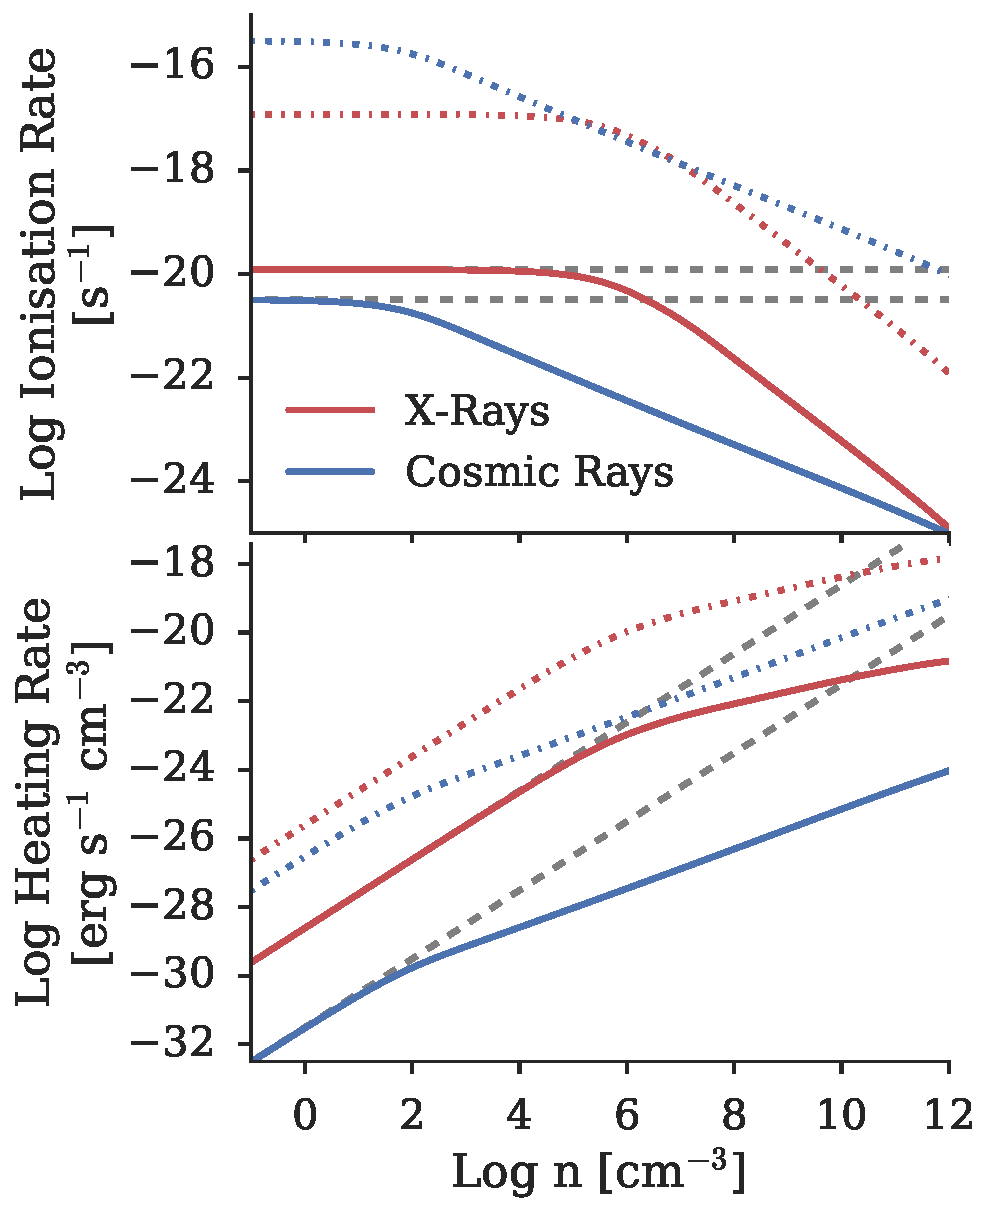
\includegraphics[width=\columnwidth]{figures/khrates/khratesCR}
\caption{\label{fig:khratesCR}
Ionisation and heating rates as a function of total gas number density for both a cosmic ray and an X-ray background at $z=25$. 
In both panels, the solid blue lines denote the rate for our fiducial CR background, $u_0$. The solid red lines show the fiducial X-ray rates from \citet{Hummeletal2015}, while the dashed grey lines demonstrate the expected rates in the absence of gas self-shielding.  
The dash-dotted blue (red) lines mark the highest-intensity CR (X-ray) heating and ionisation rates investigated. 
For a given energy density, CRs are more effective at ionising and heating the gas; vertical placement on this chart is simply a matter of normalisation, stemming from the assumptions outlined in Section \ref{sec:context}. 
Note that X-rays cause significantly more heating per ionisation event than CRs, but are strongly attenuated at high densities. CRs are significantly more penetrative in comparison.%
} 
\end{center}
\end{figure}

\begin{figure}
\begin{center}
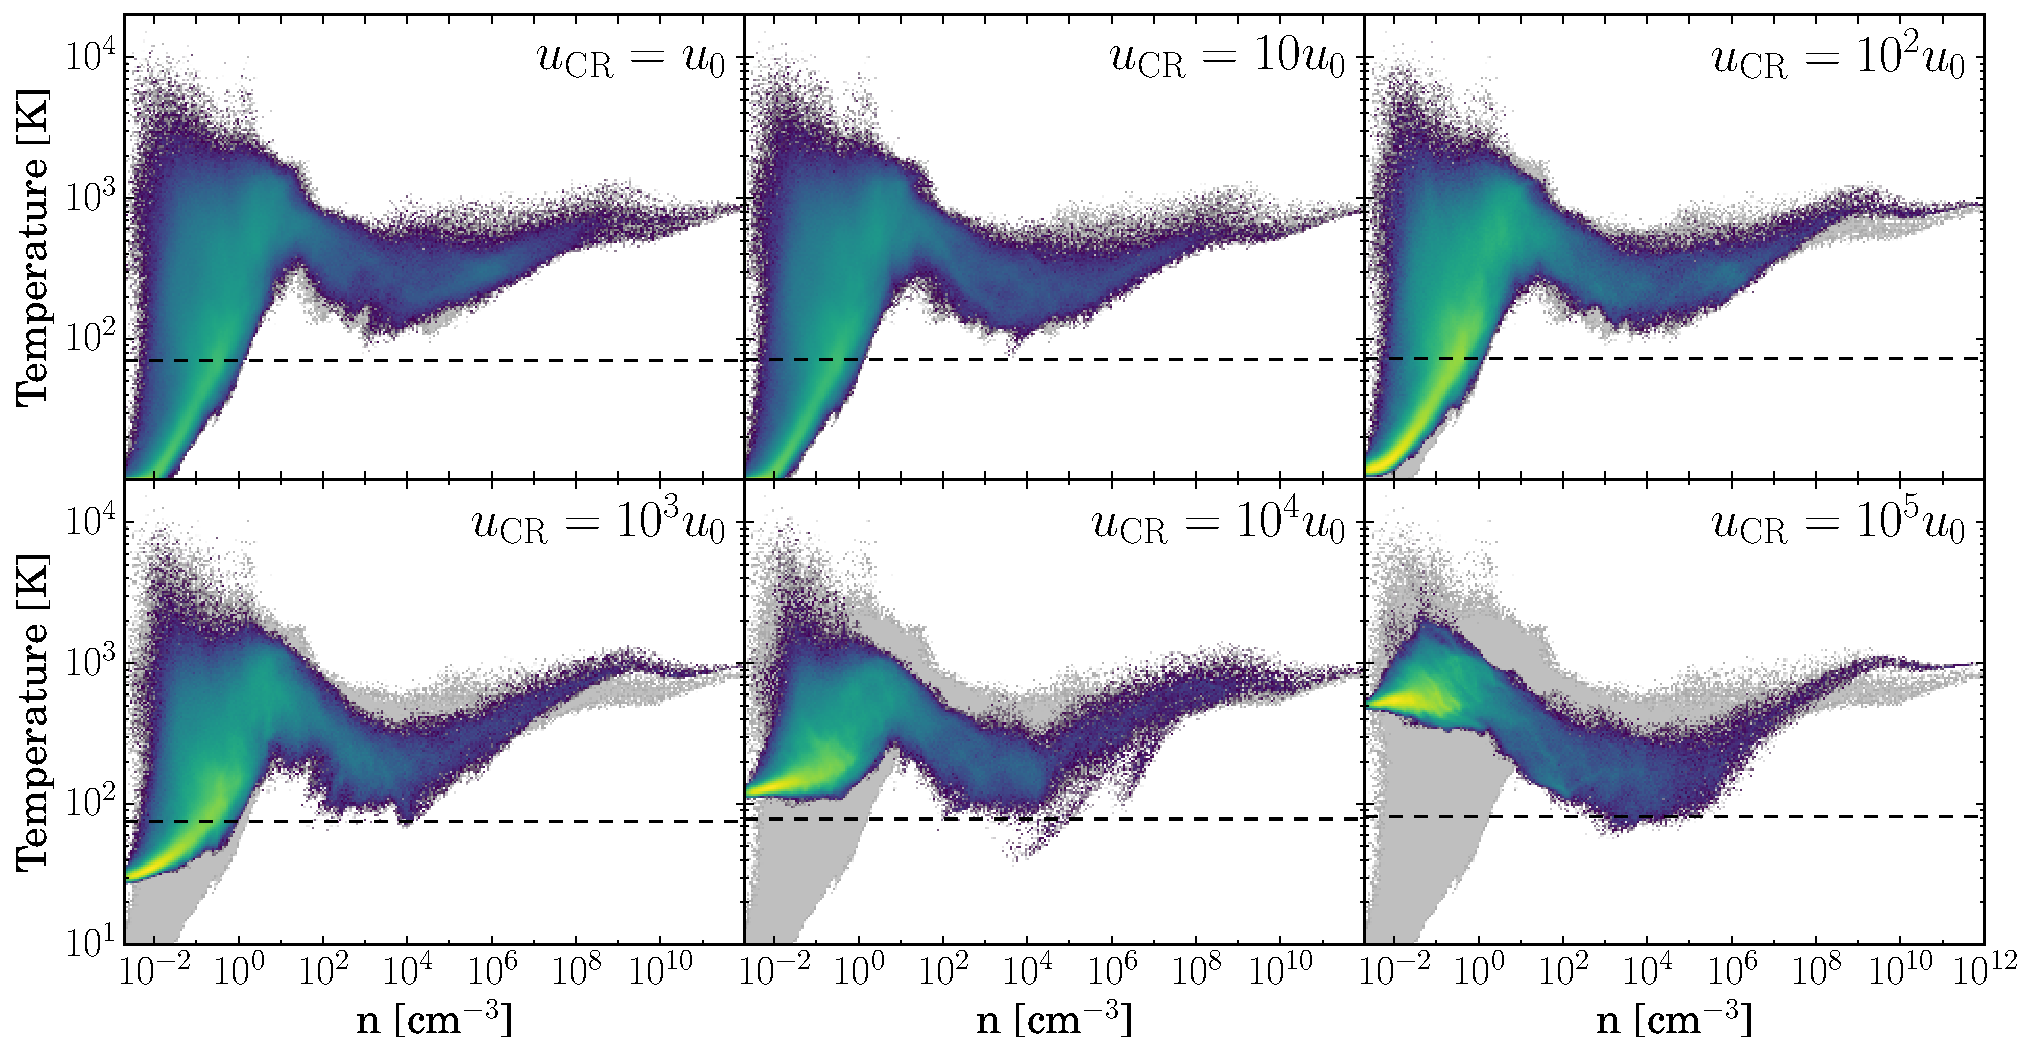
\includegraphics[width=\columnwidth]{figures/temp/temp}
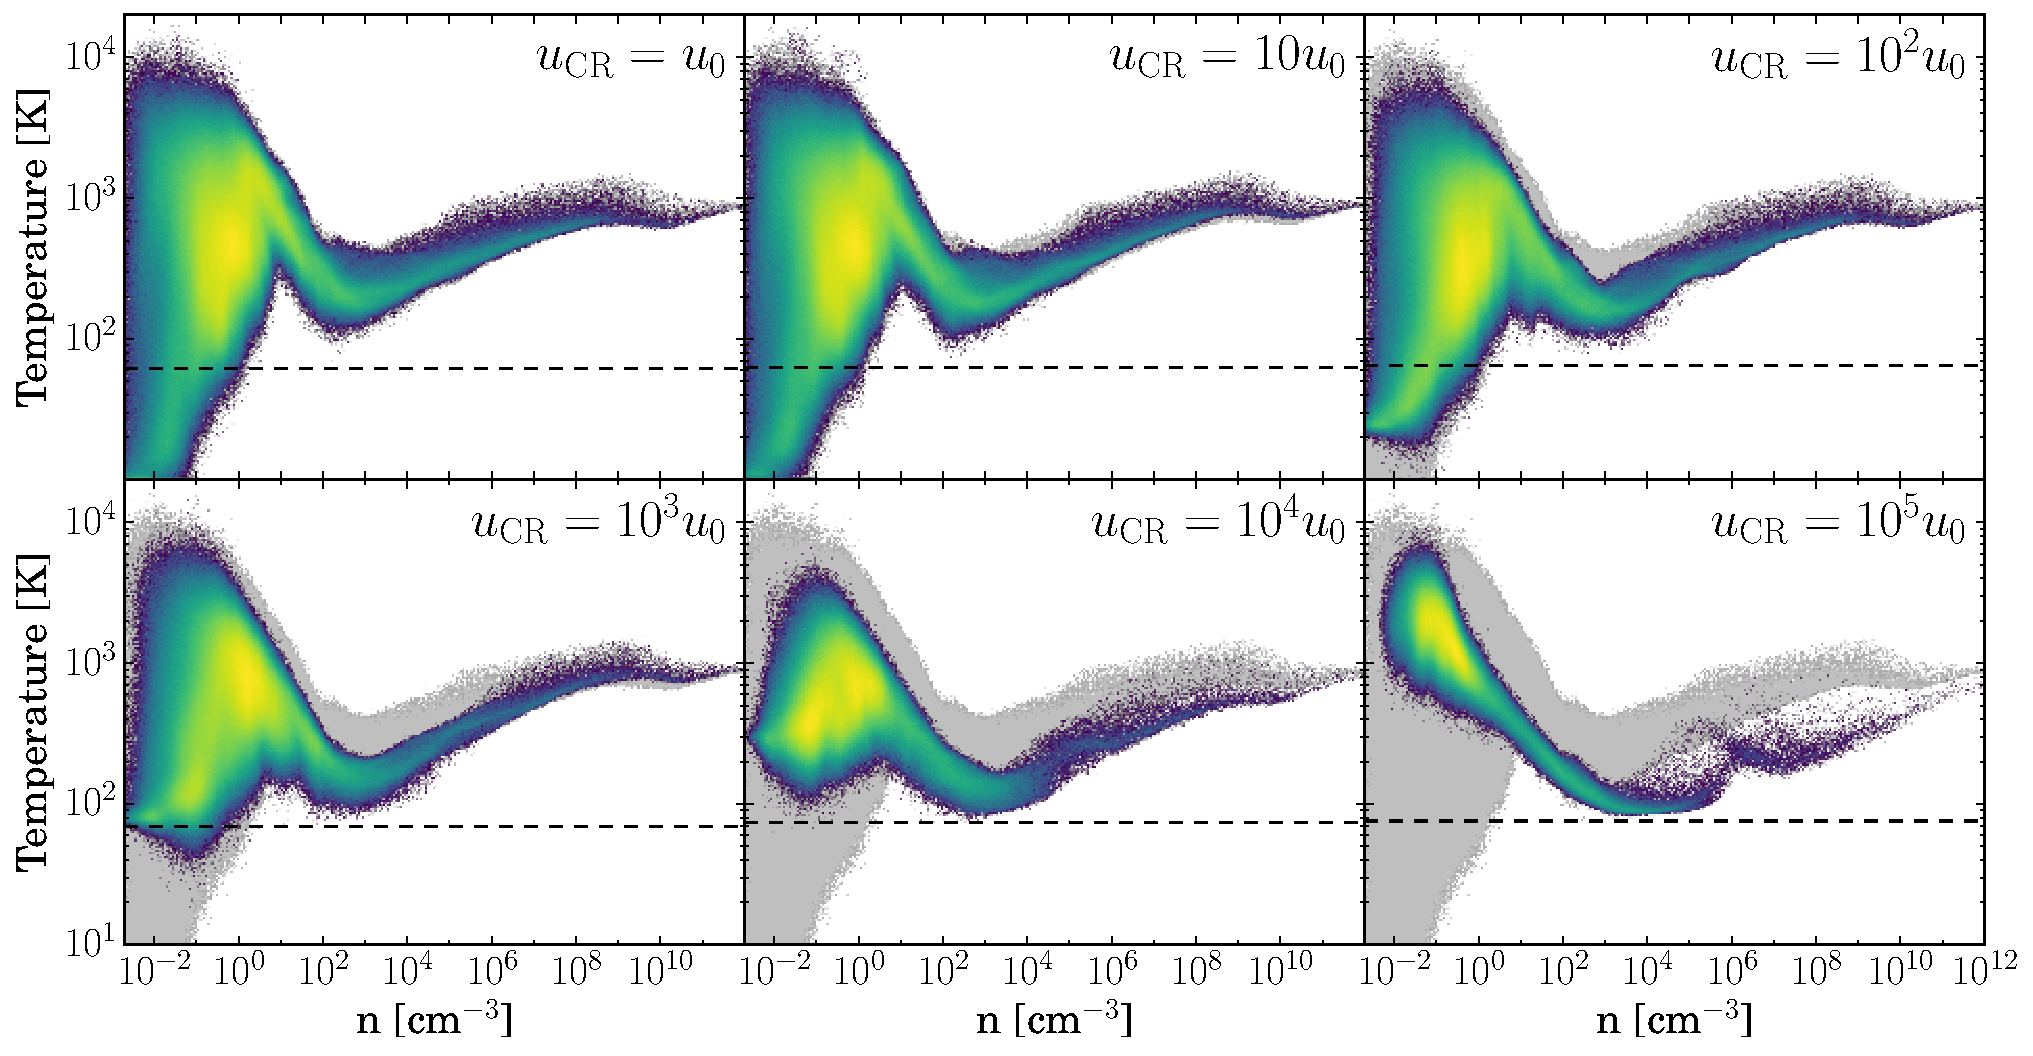
\includegraphics[width=\columnwidth]{figures/temp/temp_halo2}
\caption{\label{fig:temp}
Mass-weighted temperature-density distribution of the gas collapsing into Halo 1 (top) and Halo 2 (bottom), shown just prior to sink formation. 
Each panel shows the behaviour of gas collapsing under a CR background of a given strength. 
In each case, the behaviour of the gas in the $\ucr=0$ case is reproduced for comparison (light grey); dashed lines denote the CMB temperature when collapse occurs. Gas at low densities gets progressively hotter and gas in the loitering phase gets progressively cooler with increasing $\ucr$. 
Note that the gas invariably proceeds to collapse, and converges toward a similar thermodynamic path as it approaches sink formation densities, regardless of the CR background strength.%
}
\end{center}
\end{figure}

Accounting for this attenuation of the CR background and following the treatment of \citet{StacyBromm2007} and \citet{InayoshiOmukai2011}, the cosmic ray heating rate $\Gamma_{\mathrm \small CR}$ and ionisation rate $k_{\mathrm \small CR}$ are given by
\begin{equation}
\Gamma_{\mathrm \small CR} = 
    \frac{ E_{\mathrm \small heat}}{50\,{\mathrm \small eV}} 
    \int_{\epsilon_{\mathrm min}}^{\epsilon_{\mathrm max}} 
    \left| \left( \frac{{\mathrm d}\epsilon} {{\mathrm d}t} \right)_{\mathrm ion} \right|
    \frac{dn_{\mathrm \tiny CR}}{d\epsilon} e^{-\tau_{\mathrm \small CR}} d\epsilon,
\end{equation}
and 
\begin{equation}
k_{\mathrm \small CR} = \frac{\Gamma_{\mathrm \small CR}}{ n_{\mathrm \small H} E_{\mathrm \small heat}},
\end{equation}
where $\epsilon_{\mathrm min} = 10^6\ev$, $\epsilon_{\mathrm max}= 10^{15}\ev$, $n_{\mathrm \small H}$ is the number density of hydrogen, and $E_{\mathrm \small heat}$ is the energy deposited as heat per interaction \citep{Schlickeiser2002}.
While CRs lose about $50\ev$ per interaction, only about $6\ev$ of that goes towards heating in a neutral medium \citep{SpitzerScott1969,ShullvanSteenberg1985}; we set $E_{\mathrm \small heat}$ accordingly.

Here we assume the incident CR background is composed solely of protons, and all interactions occur with hydrogen only.  
While this neglects the slight difference in average CR energy loss per interaction for hydrogen ($36\ev$; \citealt{BakkerSegre1951}) as compared to helium ($40\ev$; \citealt{WeissBernstein1956}), the resulting error in the employed heating and ionisation rates is sufficiently small for our purposes (see \citealt{JascheCiardiEnsslin2007} for a more rigorous treatment). 

The resulting heating and ionisation rates for both the $\ucr=u_0$ and $10^5\,u_0$ cases are shown in Figure \ref{fig:khratesCR}, along with the expected rates in the absence of attenuation.
Also shown are the highest and lowest X-ray heating and ionisation rates considered in \citet{Hummeletal2015}. 
Compared to X-rays, CRs produce significantly less heating per ionisation event and penetrate to much higher densities before being attenuated; the X-ray heating and ionisation rates fall off much faster as the gas becomes optically thick.
\subsection{Sink Particles}
\label{sinkParticles}
Our sink particle method is described in \citet{StacyGreifBromm2010}. 
When a gas particle exceeds $n_{\mathrm max} = 10^{12}\cc$, it and all non-rotationally-supported particles within the accretion radius $r_{\mathrm acc}$ are replaced by a single sink particle.  
We set $r_{\mathrm acc}$ equal to the resolution length of the simulation: $r_{\mathrm acc} = L_{\mathrm res} \simeq 50\au$, where 
\begin{equation}
L_{\mathrm res} \simeq 0.5 \left( \frac{M_{\mathrm res}}{\rho_{\mathrm max}} \right)^{1/3},
\end{equation}
and $\rho_{\mathrm max} = n_{\mathrm max} m_{\mathrm H}$.  
Upon creation, the sink immediately accretes the majority of the particles within its smoothing kernel, resulting in an initial mass for the sink particle $M_{\mathrm sink}$ close to $M_{\mathrm res} \simeq 1\msun$.  
Following its creation, the density, temperature, and chemical abundances of the sink particle are no longer updated.  
The sink's density and temperature are held constant at $10^{12}\cc$ and $650\kelvin$, respectively; the pressure of the sink is set accordingly. 
Assigning a temperature and pressure to the sink particle allows it to behave as an SPH particle, thus avoiding the creation of an unphysical pressure vacuum which would artificially enhance the accretion rate onto the sink \citep[see][]{BrommCoppiLarson2002, MartelEvansShapiro2006}. 
Once the sink is formed, additional particles (including smaller sinks) are accreted as they approach within $r_{\mathrm acc}$ of that sink particle, and the position and momentum of the sink particle is set to the mass-weighted average of the pre-existing sink and the accreted particle.

\begin{figure}
\begin{center}
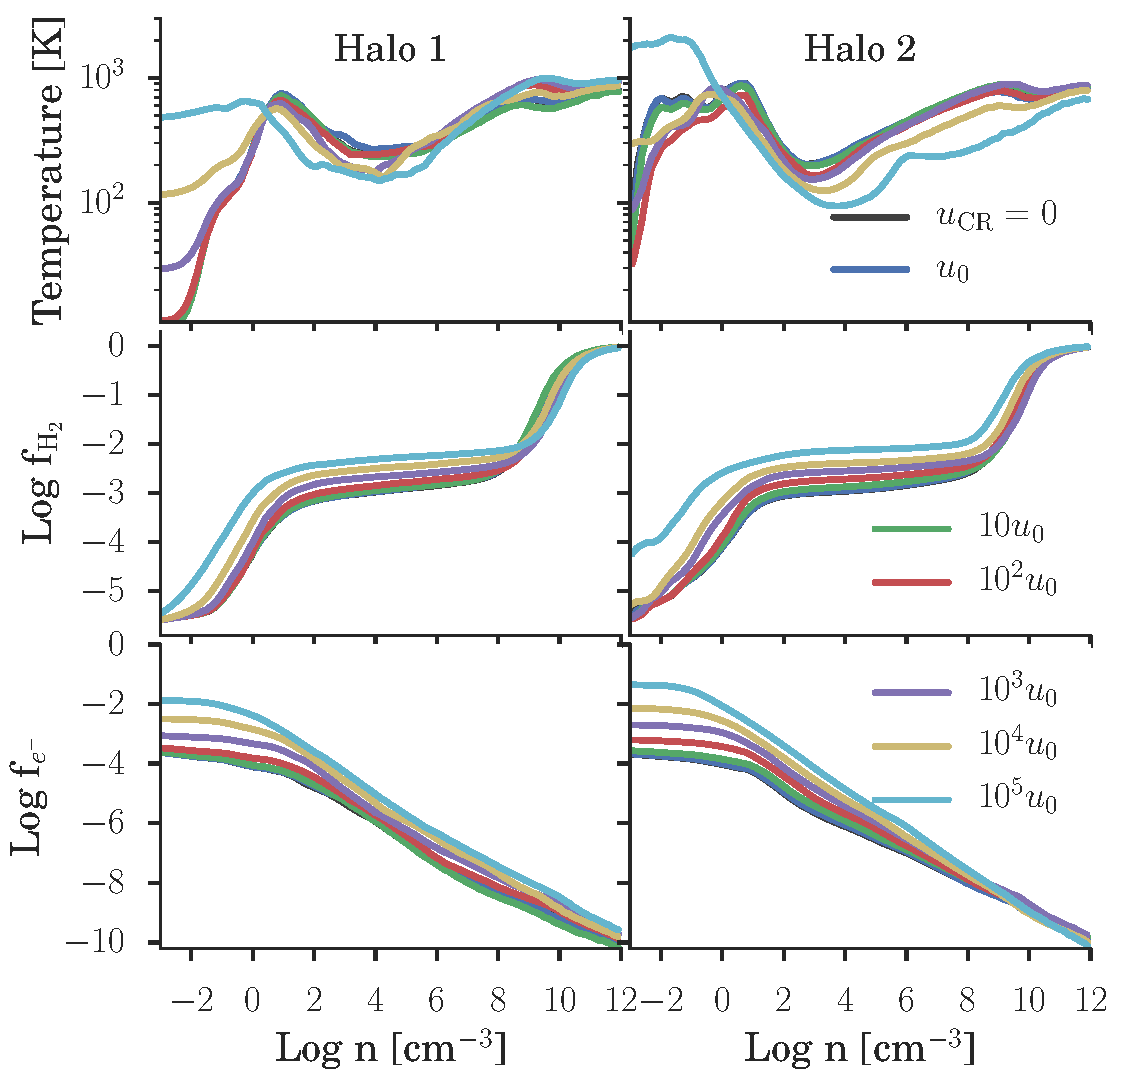
\includegraphics[width=1\columnwidth]{figures/binned_T_efrac/binned_T_efrac}
\caption{\label{fig:efrac}
From top to bottom, density-binned average gas temperature, $\htwo$ fraction, and free electron fraction for both Halo 1 (left) and Halo 2  (right). 
As $\ucr$ increases, the additional ionisation increases f$_{e^-}$, which in turn elevates f$_{\htwo}$. 
Combined with the additional heating provided by the CR background, this allows $\htwo$ cooling to activate at slightly lower densities and gas in the loitering phase to reach slightly lower temperatures, as seen in the top panel.%
}
\end{center}
\end{figure}

\begin{figure}
\begin{center}
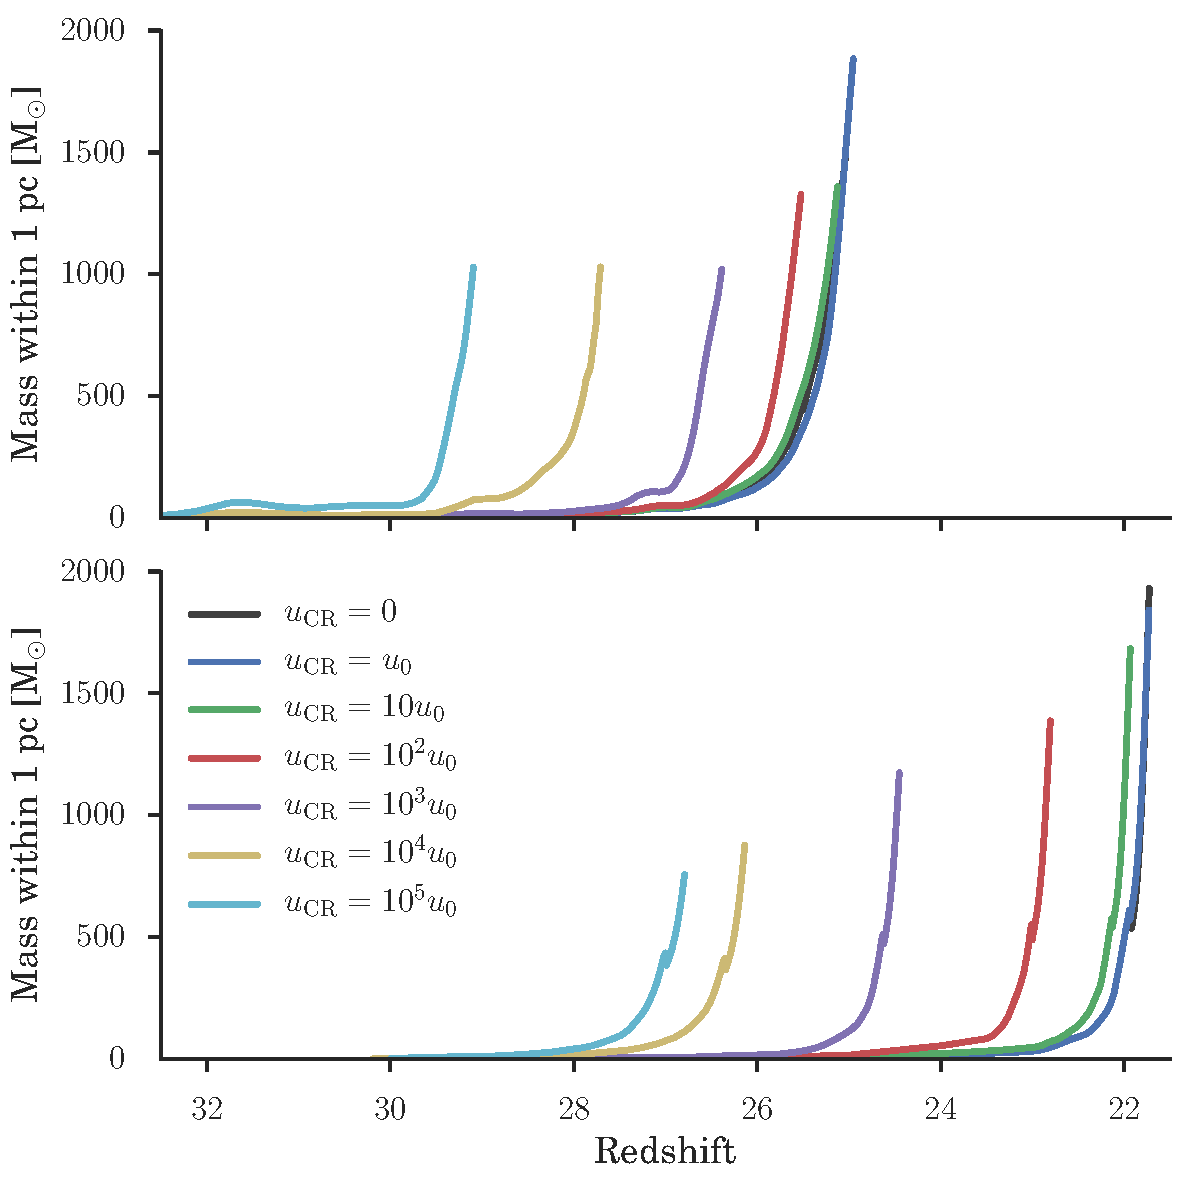
\includegraphics[width=.95\columnwidth]{figures/collapse/collapse}
\caption{\label{fig:collapse}
Total gas mass within $1\pc$ of the highest density point in each simulation over cosmic time.
Top: Halo 1; bottom: Halo 2.
As $\ucr$ increases, the additional heating and ionisation allows the gas to fulfil the Rees-Ostriker criterion ($t_{\mathrm cool} \lesssim t_{\mathrm ff}$) sooner, expediting collapse to high densities.  
The sooner runaway collapse sets in, the less time gas has to accumulate in the centre of the minihalo, resulting in a lower total mass within $1\pc$ at simulation's end.
The discontinuity seen in the growth of Halo 2 is a numerical artefact arising from the cut-out and refinement process.%
}
\end{center}
\end{figure}

\section{Results}
\label{sec:results}
\subsection{Initial Collapse}
\subsubsection{CR-enhanced H$_2$ Cooling}
\label{sec:initial_collapse}

The gas in both Halo 1 and Halo 2 invariably collapses to high densities, even as we vary the CR background strength by five orders of magnitude. 
As seen in Figure \ref{fig:temp}, the collapse occurs in accordance with the standard picture of Pop III star formation \citep[e.g.,][]{Greifetal2012,StacyBromm2013,Hiranoetal2014,Hosokawaetal2015}, albeit slightly modified by the presence of a CR background.  
In each case, the gas heats adiabatically as it collapses until reaching $\sim10^3\kelvin$, at which point $\htwo$ cooling is activated.  
This allows the gas to cool to $\sim200\kelvin$, whereupon it enters a `loitering' phase \citep{BrommCoppiLarson2002}, increasing in density quasi-hydrostatically until sufficient mass accumulates to trigger the Jeans instability, typically between $10^4\cc$ and $10^6\cc$. 
Runaway collapse then proceeds until three-body reactions become important at $n\sim10^8\cc$; this turns the gas fully molecular by $n\sim10^{12}\cc$, at which point we insert sink particles.

As demonstrated in Figure \ref{fig:efrac}, increasing $\ucr$ both heats the gas and boosts the resulting ionisation fraction.
This in turn increases the efficiency of $\htwo$ formation, enhancing cooling and allowing gas in the loitering phase to reach progressively lower temperatures. 
In fact, the additional cooling is sufficient to cool the gas all the way to the CMB floor when $\ucr \gtrsim 10^4\,u_0$. 
However as the gas exits the loitering phase and proceeds to higher densities, the CR optical depth increases significantly. 
In concert with the onset of three-body processes this renders CR ionisation and heating ineffective at high densities. 
As a result, the thermal behaviour of the gas increasingly resembles that seen in the $\ucr=0$ case as the collapse proceeds. 
To wit, by the time we form sink particles at  $10^{12}\cc$ the thermodynamic state of the gas is remarkably similar, even as we vary the CR background strength by five orders of magnitude.
This convergence under a wide range of environmental conditions is similar to that seen in the presence of both an X-ray background \citep{Hummeletal2015} and DM--baryon streaming \citep{StacyBrommLoeb2011a,Greifetal2011b}.

\begin{figure}
\begin{center}
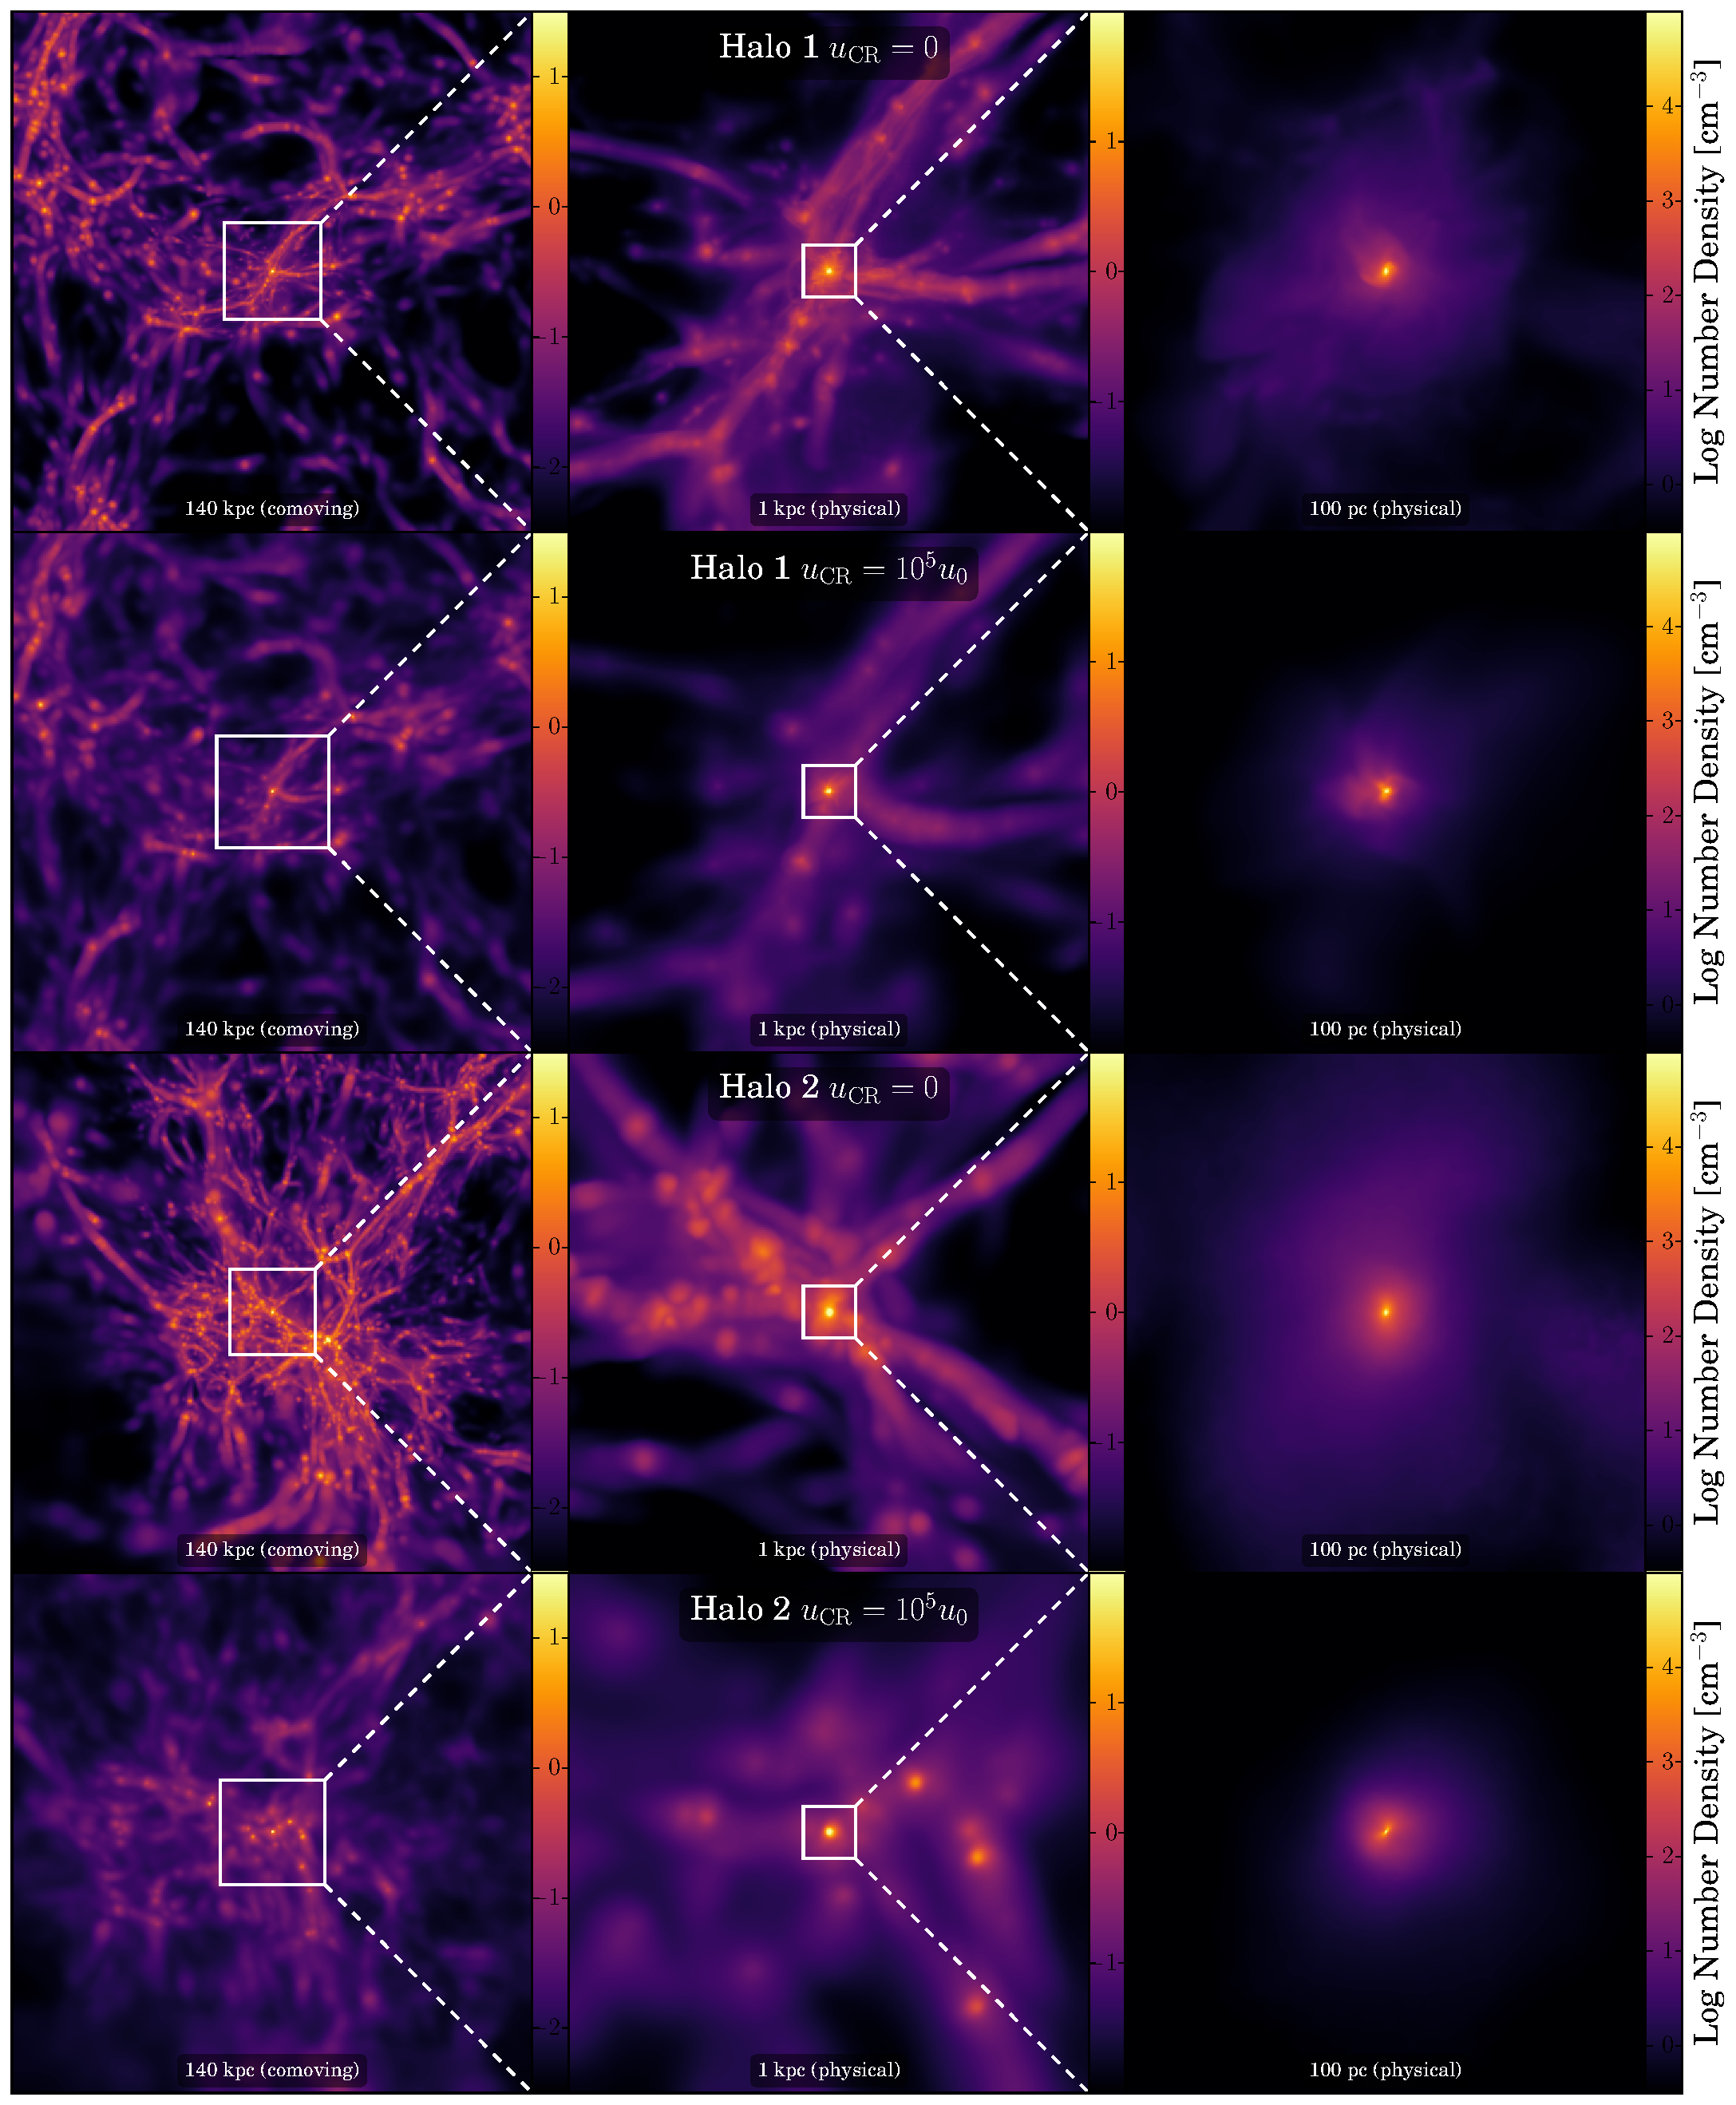
\includegraphics[width=\columnwidth]{figures/structure/structure}
\caption{\label{fig:structure}
Simulation structure for both Halo 1 (top) and Halo 2 (bottom) as seen in the final output, $5000\yr$ after the first sink forms.  
Shown is a density projection of the minihalo environment on progressively smaller scales for both the $\ucr=0$ and $\ucr=10^5\,u_0$ simulations, as labelled.  
White boxes indicate the region depicted on the next smaller scale.  
From left to right: filamentary structure of the cosmic web near the minihalo formation site; minihalo formation at the intersection of several filaments; morphology within the $\sim$$100\pc$ virial radius of the minihalo. 
The density scale for each level is shown just to the right -- note that the scaling changes from panel to panel.
Note how the gas in the $\ucr=10^5\,u_0$ simulations appears smoothed out compared to the $\ucr=0$ simulations.  
Not only do CRs heat and smooth the filamentary gas, the expedited collapse induced by CR ionisation leaves less time for low-density structure to form, since the collapse is shifted to an earlier epoch.  
As a result, the dynamical environment in which the sink particles form varies significantly between simulations.%
}
\end{center}
\end{figure}

\begin{figure}
\begin{center}
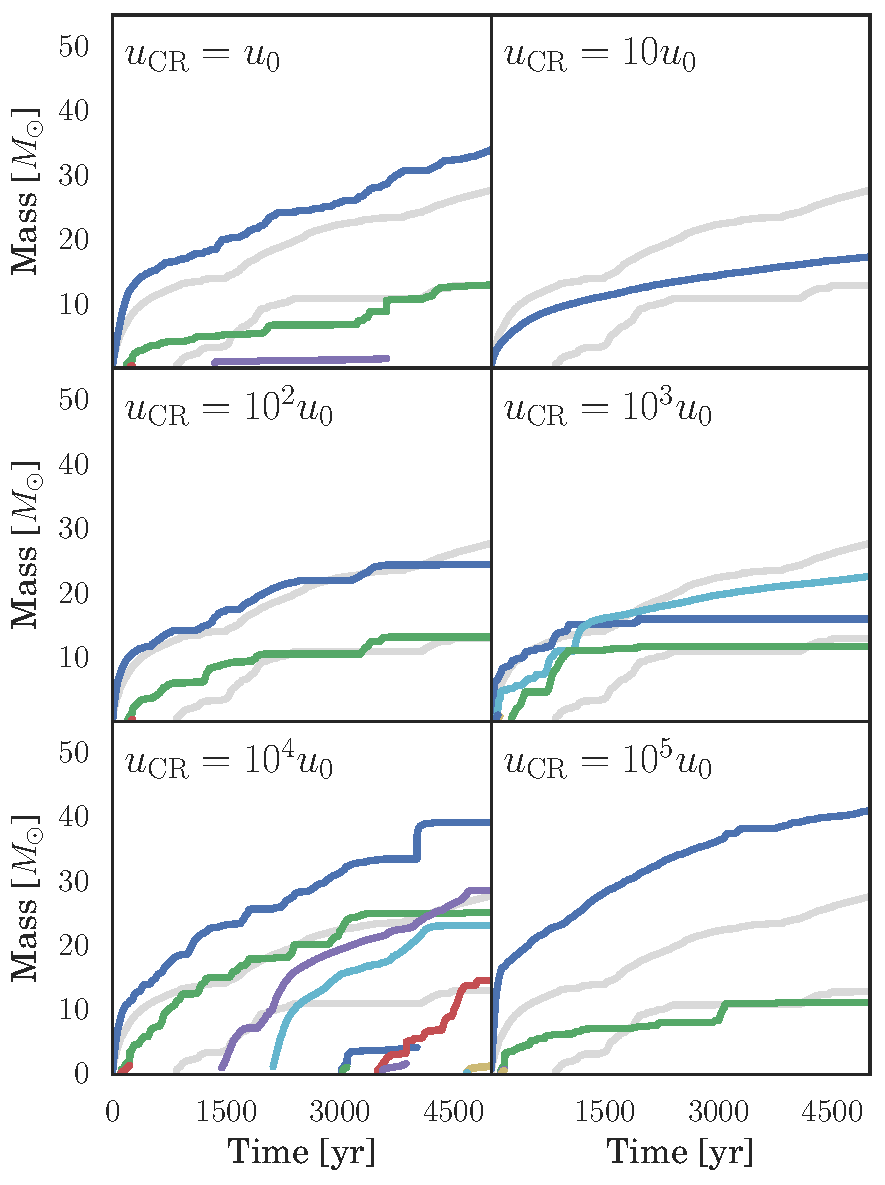
\includegraphics[width=.49\textwidth]{figures/sink_masses/sink_masses_halo1}
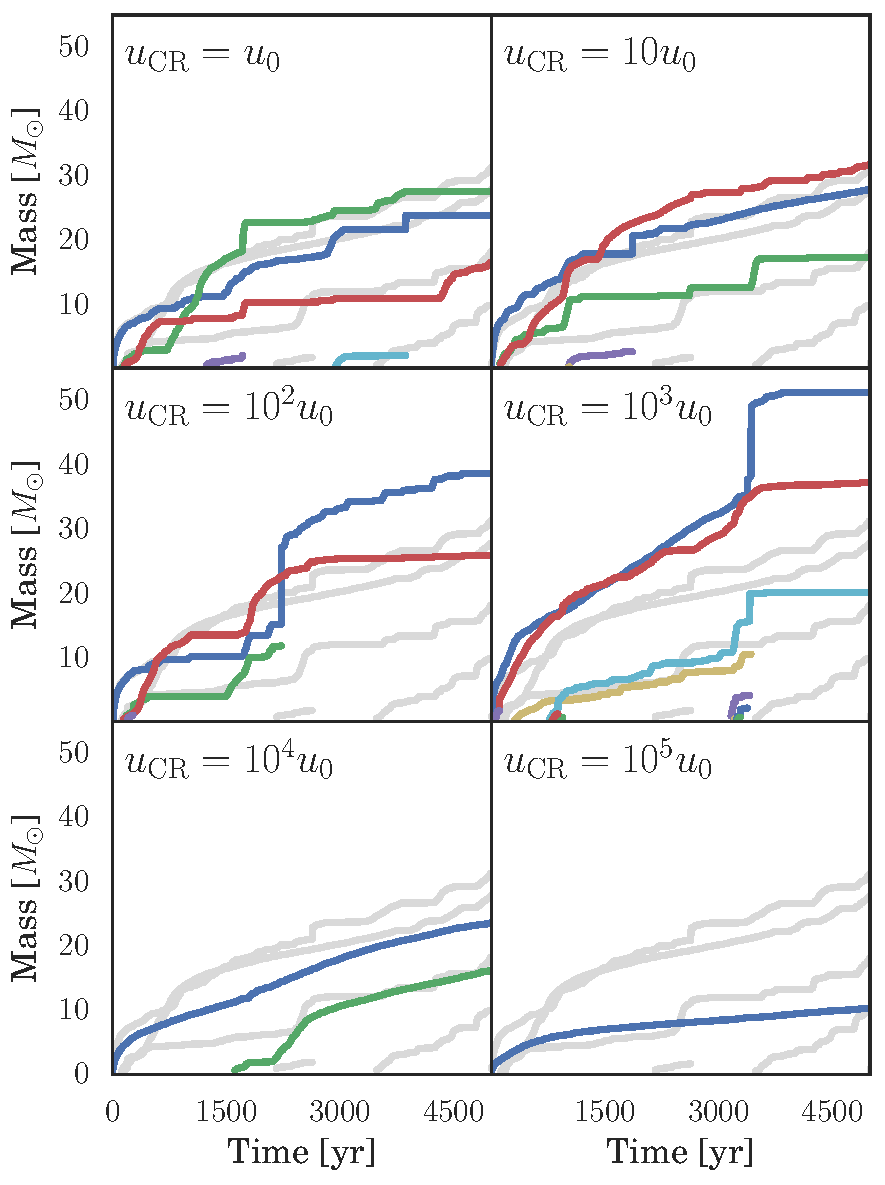
\includegraphics[width=.49\textwidth]{figures/sink_masses/sink_masses_halo2}
\caption{\label{fig:sinks} 
Growth of individual sink particles in each simulation over time, with the first sink forming at $t=0$. 
Lines end where one sink is accreted by another. 
The Halo 1 suite of simulations is shown in the left panel, Halo 2 in the right panel.  
The growth of the sinks in the corresponding $\ucr=0$ is shown in grey in the background of each panel for comparison. 
There are no apparent trends with increasing $\ucr$ -- neither in typical sink mass nor in the number of fragments formed.%
}
\end{center}
\end{figure}

\subsubsection{Expedited Collapse}
\label{sec:expedited_collapse}
Boosting the $\htwo$ fraction in the gas lowers the density threshold for efficient cooling, allowing the gas to fulfil the Rees-Ostriker criterion sooner by driving the cooling time $t_{\mathrm \small cool}$ below the freefall time $t_{\mathrm \small ff}$ \citep{ReesOstriker1977}.
This is demonstrated in Figure \ref{fig:efrac}, where we see the density at which the gas begins to cool drop as the CR background strength increases.  
This necessarily expedites the subsequent phases of the collapse, as seen clearly in Figure \ref{fig:collapse}, where we show the total gas mass within 1 pc (physical) of the minihalo's centre as a function of redshift.  
The impact this has on the environment in which the minihalo collapses is seen in Figure \ref{fig:structure}, where we show the final simulation output on various scales for Halo 1 and Halo 2, both in the absence of any CR background ($\ucr=0$) and with $\ucr=10^5\,u_0$. 
Low density filamentary gas is heated and prevented from collapsing, reducing the clumping of the IGM and possibly impacting the early stages of reionisation.
Gas above a $\ucr$-dependent density threshold on the other hand experiences enhanced cooling and thus has its collapse expedited.
As a result, the dynamical environment in which the first sink particles form varies significantly depending on the strength of the CR background.

\begin{figure}
\begin{center}
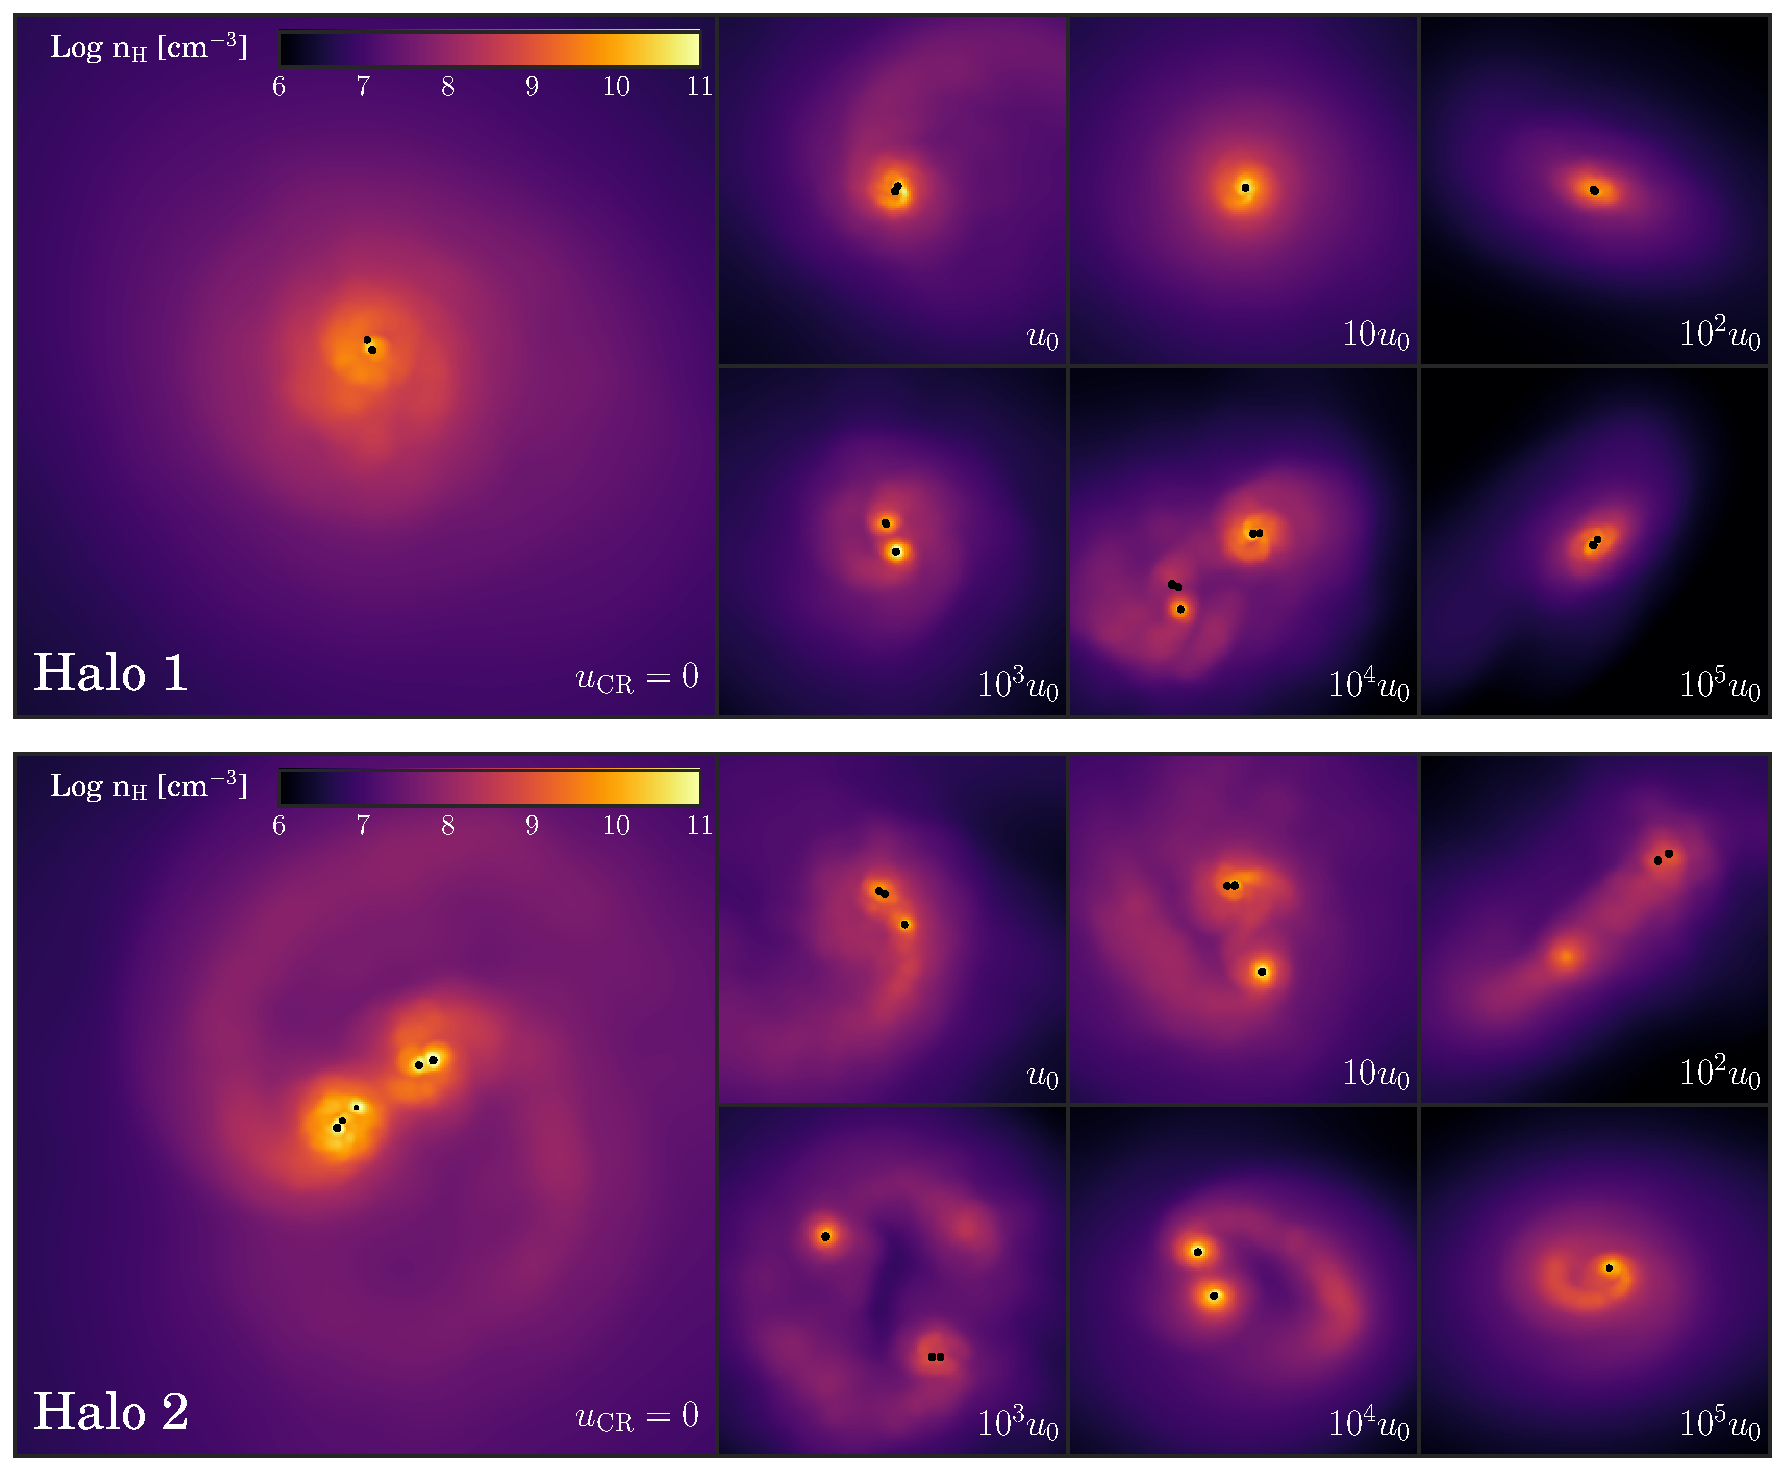
\includegraphics[width=\columnwidth]{figures/disks/disks}
\caption{\label{fig:disks} 
Density projection of the central $20\,000\au$ of each simulation $5000\yr$ after the formation of the first sink particle.
Upper panel: Halo 1; lower panel: Halo 2.
Each accretion disc is shown face-on; sink particle positions are identified by black dots whose size scales logarithmically with the mass of the sink.
In each panel the accretion disk formed in the absence of any CR background is shown on the left; the corresponding $\ucr$-modified discs are shown to the right.
Note the broad variation in both disc structure and spatial extent.%
}
\end{center}
\end{figure}

\subsection{Star Formation}
\subsubsection{Protostellar Fragmentation and Growth}
\label{sec:sink_formation}

Figure \ref{fig:sinks} shows the growth over time of all sink particles formed in our simulations, from formation of the first sink particle to simulation's end $5000\yr$ later when radiative feedback can no longer be ignored. 
The first sink particle forms when the gas in the centre of the minihalo reaches densities of $10^{12}\cc$, and develops an accretion disk within a few hundred years. 
In all but three cases, this disk quickly fragments, forming a binary or small multiple within $500\yr$. 
Sinks that survive longer than a few hundred years without undergoing a merger quickly accrete the surrounding gas, growing to $\sim$a few solar masses within $500\yr$ and typically reaching between 10 and $40\msun$ by simulation's end.

As is evident from Figure \ref{fig:sinks}, there is no clear trend with $\ucr$ in either protostellar growth or accretion rate, nor is there any trend in the total sink mass.
For example, both the $10\,u_0$ Halo 1 simulation and $10^5\,u_0$ Halo 2 simulation form only a single sink while the $10^3\,u_0$ Halo 2 simulation steadily forms a total of 14 sink particles over the $5000\yr$ period.
This  can be primarily attributed to the wide variety of dynamical environments in which the sink particles form---demonstrated in Figure \ref{fig:disks}, where we show the accretion disk structure of each simulation $5000\yr$ after the first sink formed.
This variation is a direct consequence of the expedited collapse discussed in Section \ref{sec:expedited_collapse}. 
As seen in Figure \ref{fig:structure}, expediting the initial collapse results in significant variation of the experienced gravitational potential; the collapse history of the gas and the dynamical environment in which the sinks form varies accordingly.
Given the lack of any apparent trends with increasing $\ucr$, this suggests the final stages of the collapse are influenced more by small-scale turbulence than the strength of the CR background.
While CRs may indeed alter the susceptibility of the disk to fragmentation, any such behaviour is masked by variations in the collapse history between simulations.

\begin{figure}
\begin{center}
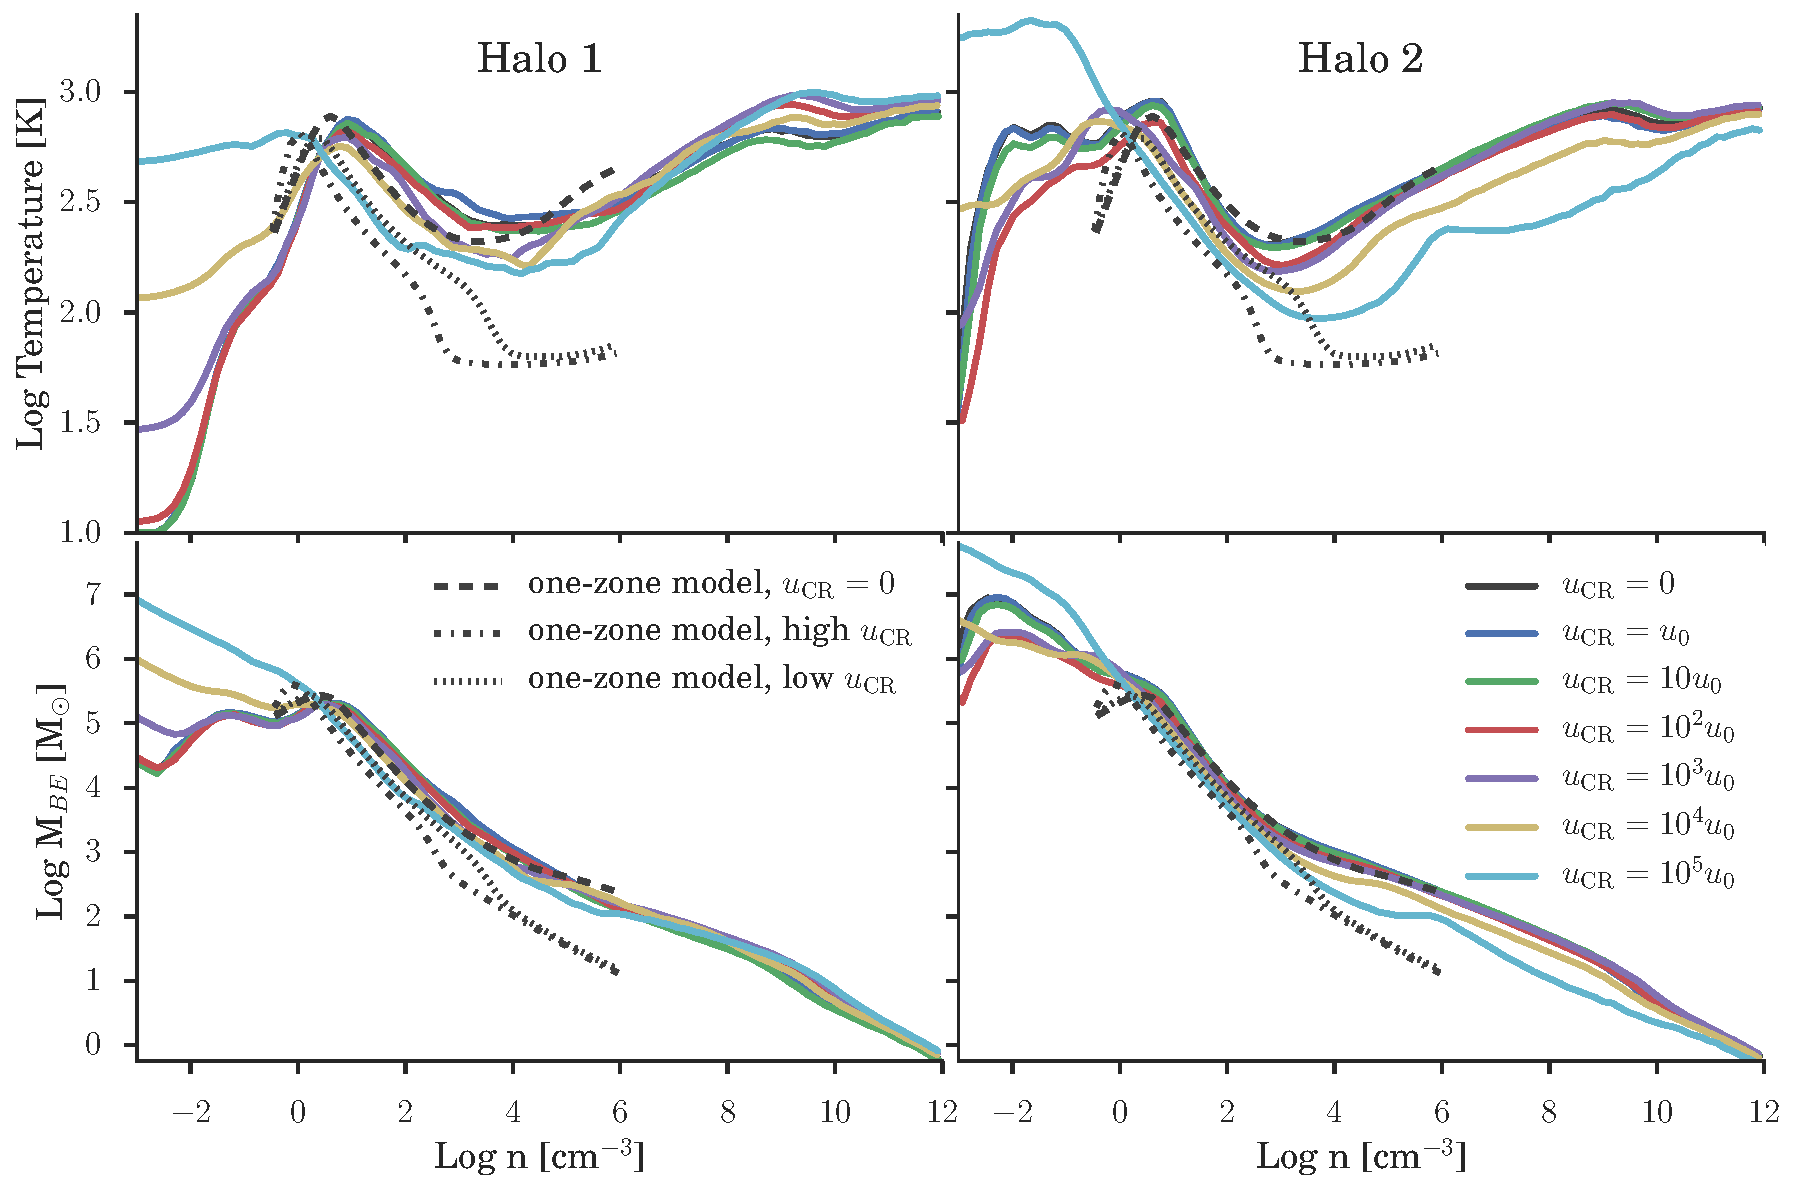
\includegraphics[width=\columnwidth]{figures/binned_T_Mbe/binned_T_Mbe}
\caption{\label{fig:Mbe}
Density-binned average temperature (top) and Bonnor-Ebert mass (bottom) for Halo 1 (left) and Halo 2 (right) for all CR background strengths, as labelled.
Overlaid on each panel are the one-zone calculations of \citet{StacyBromm2007}, which only tracked the gas evolution up to densities of $10^6\cc$, insufficient to observe the $\ucr$-independent convergence in the thermodynamic state of the gas as it proceeds to runaway collapse.%
}
\end{center}
\end{figure}

\subsubsection{Characteristic Mass}

While the final stages of the collapse appear to be somewhat chaotic, with protostellar fragmentation driven primarily by small-scale turbulence rather than the CR background, the typical mass of the sinks formed remains quite stable across all simulations at $10-40\msun$.
This is very much in line with the prevailing consensus for the expected mass of the first stars in the absence of any radiative feedback of $\sim$ a few $\times10\msun$ \citep{Bromm2013}.  
As noted in Section \ref{sec:initial_collapse}, the thermodynamic behaviour of the gas displays a remarkable similarity as it approaches sink formation densities, regardless of $\ucr$.
This suggests that the influence of the CR background is restricted to lower densities, with little to no effect on the protostellar cores from which the first stars ultimately form.

The universality of this characteristic mass is further supported by Figure \ref{fig:Mbe}, where we show the average gas temperature as a function of number density, as well as the approximate fragmentation mass scale, as estimated by the Bonnor-Ebert mass \citep[e.g.,][]{StacyBromm2007}:
\begin{equation}
    M_{\mathrm \small BE} = 700\msun \left(\frac{T}{200\kelvin}\right)^{3/2}
                                 \left(\frac{n}{10^4\cc}   \right)^{-1/2},
\end{equation}
where $n$ and $T$ are the number density and corresponding average temperature.
Approaching sink formation densities $M_{\mathrm \small BE}$ is nearly independent of $\ucr$, in agreement with the observed lack of evolution in the sink mass.

Also shown in Figure \ref{fig:Mbe} are the one-zone calculations from \citet{StacyBromm2007}.
Investigating the impact of a CR background on Pop III star formation in a $z=21$ minihalo using the CR background strengths shown in Figure \ref{fig:ucr}, their models suggested 
that a sufficiently strong background might decrease the fragmentation mass scale by an order of magnitude as a result of the cooler temperatures experienced during the loitering phase.
While we observe similar behaviour from gas in the loitering phase, once the gas proceeds to runaway collapse its thermodynamic state quickly converges with that of the $\ucr=0$ case, such that the fragmentation mass scale remains unaltered.
Unfortunately the models of \citet{StacyBromm2007} only followed the gas evolution up to densities of $10^6\cc$, insufficient to observe this convergent behaviour.

\section{Summary and Conclusions}
\label{conclusions}

We have performed two suites of cosmological simulations employing a range of CR backgrounds spanning five orders of magnitude in energy density. 
We follow the thermodynamic evolution of the gas as it collapses into a minihalo from IGM densities up to $n=10^{12}\cc$, at which point three-body processes have turned the gas fully molecular. 
This allows us to capture the combined impact of CR heating and ionisation on Pop III stars forming in the minihalo via its influence on $\htwo$ and $\hd$ cooling.
Once the gas reaches $n=10^{12}\cc$, we form sink particles and follow the subsequent evolution of the system for $5000\yr$, after which point radiative feedback from the forming protostars can no longer be ignored, and our simulations are terminated.

While it also serves to heat the gas, the primary impact of the CR background is to increase the number of free electrons in the collapsing gas, catalysing the formation of additional molecular hydrogen, which in turn enhances the $\htwo$ cooling efficiency.  
This decreases the cooling time, allowing the gas to fulfil the Rees-Ostriker criterion sooner and expediting minihalo collapse. 
Each simulation therefore collapses to high density at a different epoch, and the resulting variation in experienced gravitational potential causes the collapse history---and thus the accretion disk structure---to differ greatly between simulations.

Our first suite of simulations (Halo 1) used the same initial conditions as our prior investigation of a cosmic X-ray background \citep{Hummeletal2015}, allowing for a direct comparison of the results.
CRs are much less efficient than X-rays at heating the gas, such that the collapse suppression observed for a sufficiently strong X-ray background does not occur here.  
While expedited collapse is observed in the presence of an X-ray background as well, the effect is somewhat more pronounced here owing to the more efficient nature of CR ionisation, as there is less associated heating to partially counteract the enhanced cooling.

Our second suite of simulations focused on a minihalo collapsing at $z\simeq21.5$ in the $\ucr=0$ case in order to allow a more direct comparison to the results of \citet{StacyBromm2007}, and control for the influence of the CMB temperature floor on our results.
While we find similar evidence for a lower gas temperature in the loitering phase, extending our study beyond the $n=10^6\cc$ limit of \citet{StacyBromm2007} revealed that the thermodynamic path of the collapsing gas---and thus, the fragmentation mass scale---begins to converge with that of the $\ucr=0$ case for $n\gtrsim10^6\cc$.  
This convergence is observed in all simulations for both Halo 1 and Halo 2, with the thermodynamic state of the gas becoming nearly independent of $\ucr$ by the time we form sink particles at $n=10^{12}\cc$.
The remarkable similarity in the thermodynamic state of the gas just prior to sink formation suggests the presence of a CR background has little impact on the characteristic mass of the stars formed.  
Indeed, the typical mass of the sink particles formed is quite robust, remaining stable across all simulations at $10-40\msun$, very much in line with the expected mass of the first stars in the absence of external radiative feedback. In fact, this robust behaviour is observed under a variety of environmental conditions, including X-ray irradiation \citep{Hummeletal2015} and DM--baryon streaming \citep{StacyBrommLoeb2011a,Greifetal2011b}.

While the neutral impact of the CR background on the thermodynamic state of primordial gas at high densities results in a robust characteristic mass that does not vary with $\ucr$, there is a possibility that the enhanced cooling resulting from CR ionisation may decrease the velocity dispersion of the infalling gas \citep{Clarketal2011a}.  
This would decrease fragmentation in the centre of the minihalo, possibly increasing the mass of the stars formed.
While we see no evidence to support this, any such systematic effect could be easily masked by the variations in collapse history between simulations.  
Likewise, the fact that each simulation collapses to high densities at a different epoch in a different gravitational potential well limits our ability to draw detailed conclusions regarding the impact of the CR background on fragmentation in the protostellar accretion disc.

Finally, while the characteristic mass---and thus, ionising output---of Pop III stars appears to be unaffected by the presence of a CR background, CRs still heat the low-density gas in the IGM, reducing its clumping factor. This may have implications for reionisation and the 21-cm signal \citep{FurlanettoPengBriggs2006, SazonovSunyaev2015}.

\chapter{The Source Density and Observability of Pair-Instability Supernovae from the First Stars}

\section{Introduction}
Understanding the formation of the first stars and galaxies is one of
the central challenges of modern cosmology, as they mark a significant
increase in complexity from the simple initial conditions of the
primordial universe during the `dark ages' (e.g.,
\citealt{BarkanaLoeb2001, Miralda-Escude2003, Brommetal2009,
  Loeb2010}). The basic properties of these so-called Population III
(Pop~III) stars have been reasonably well established, with the
consensus that the first stars formed in dark matter `minihalos' on
the order of $10^5$--$10^6$\msun at high redshifts
\citep{CouchmanRees1986,HaimanThoulLoeb1996,Tegmarketal1997}.
Numerical simulations of the collapse of primordial metal-free gas
into these halos, where molecular hydrogen is the only available
coolant, had suggested that the first stars were predominantly very
massive, with $M_* \gtrsim100$\msun and a top-heavy initial mass
function (IMF) (e.g., \citealt{BrommCoppiLarson1999,
  BrommCoppiLarson2002, AbelBryanNorman2002, BrommLarson2004,
  Yoshidaetal2006, O'SheaNorman2007}).  More recent work has found
that the gas from which the first stars formed underwent significant
fragmentation \citep{StacyGreifBromm2010, Clarketal2011b,
  Greifetal2011, Greifetal2012}, and experienced strong protostellar
feedback \citep{Hosokawaetal2011, StacyGreifBromm2012}.  These results
have revised our picture of Pop~III star formation, with lower
characteristic masses (on the order of 50 rather than $100$\msun) and
a much broader IMF now expected.  The light from these stars ended the
dark ages and fundamentally transformed the universe, beginning both
the reionization (e.g, \citealt{Meiksin2009}) and the chemical
enrichment of the universe (e.g, \citealt{Karlsson2011}).

Given the top-heavy nature of Pop~III star formation and the fact that
low-metallicity stars are unlikely to undergo significant radiatively
driven mass loss \citep{Kudritzki2002}, one interesting possibility is
that some of the first stars died as pair-instability supernovae
(PISNe), a scenario that has significant consequences for the chemical
enrichment history of the universe \citep{HegerWoosley2002,
  TumlinsonVenkatesanShull2004, KarlssonJohnsonBromm2008}.  Basic
one-dimensional models predict that stars with masses in the range
140--260\msun will undergo a pair-production instability and explode
completely \citep{BarkatRakavySack1967, Fraley1968}.  During core
oxygen burning, a combination of high temperatures and relatively low
densities results in the formation of $e^{\pm}$ pairs, removing
pressure support from the core. Following the subsequent contraction,
the ignition of explosive oxygen burning completely disrupts the
progenitor, resulting in a significant contribution to the metal
enrichment of the surrounding medium. More recently,
\citet{ChatzopoulosWheeler2012} and \citet{YoonDierksLanger2012} have
found that stars with initial masses as low as 65\msun can encounter
the pair-production instability if they are rapidly rotating.  In this
scenario, strong rotationally induced mixing causes nearly homogeneous
evolution, such that the star is converted almost entirely to helium
before the next phase in its evolution begins.  These extremely
energetic explosions|approaching $10^{53}$ ergs for the most massive
models|are very luminous, in part due to the large amount of $^{56}$Ni
produced, and are also very temporally extended as a result of the
large mass ejected \citep{FryerWoosleyHeger2001, HegerWoosley2002,
  Hegeretal2003, JoggerstWhalen2011, KasenWoosleyHeger2011}.

A second possiblility for reaching such extreme explosion energies in
slightly lower mass stars is the hypernova scenario for rapidly
rotating stars that undergo core collapse \citep{UmedaNomoto2003,
  TominagaUmedaNomoto2007}.  During the collapse, accretion onto a
central black hole powers a jet which induces a highly energetic
explosion. While recent work has decreased the expected mass of the
first stars, they have also been found to rotate more rapidly than
previously thought \citep{StacyBrommLoeb2011}, increasing the
plausibility of this scenario. Evidence supporting this hypothesis has
recently been presented by \citet{Chiappinietal2011}.

While not an example of a Pop~III star, the recent discovery of the
extremely luminous supernova (SN) 2007bi, identified as a possible
PISN, in a metal-poor dwarf galaxy at a redshift of $z\simeq0.1$
\citep{Gal-Yametal2009} suggests that PISNe may be possible in the
local universe under rare circumstances. Further supporting this
picture, \citet{WoosleyBlinnikovHeger2007} have shown that SN 2006gy
\citep{Smithetal2007} is well modeled by a pulsational
pair-instability model. For stars with initial masses in the range
$\sim$100--140\msun, the star encounters the $e^{\pm}$ production
instability, but the resulting explosive ignition of oxygen is
insufficient to unbind the star.  Instead it ejects a shell of
material before settling back into a stable configuration.  The star
encounters this instability several times until the mass of the helium
core drops below $\sim$40\msun, after which the star can proceed to
silicon burning and eventually undergo core-collapse.

With the upcoming launch of the \textit{James Webb Space Telescope}
(JWST) we will be able to probe the epoch of first light in
unprecedented detail.  While the first stars themselves are unlikely
to be visible (e.g, \citealt{BrommKudritzkiLoeb2001,
  PawlikMilosavljevicBromm2011}), some of the SNe that end their lives
should be within the detection limits of the JWST (e.g.,
\citealt{MackeyBrommHernquist2003, Scannapiecoetal2005,
  Gardneretal2006}). While the basic properties of PISNe and the
effect they have on their environment has been well studied
\citep{MoriFerraraMadau2002, BrommYoshidaHernquist2003,
  FurlanettoLoeb2003, KitayamaYoshida2005, Whalenetal2008,
  WiseAbel2008, Greifetal2010}, the source density of these events has
yet to be well constrained.

The first attempt at estimating the number and observability of SNe at
high redshift was made by \citet{Miralda-EscudeRees1997}, who
calculated the all-sky SN rate based on estimates of the total metals
produced by a typical SN and the observed metallicity of the
intergalactic medium (IGM) at high redshifts.  This yields $\sim$1 SN
yr$^{-1}$ arcmin$^{-2}$ at $z \sim 5$. Other early work attempted to
model the SN rate based on the empirically determined star formation
rate out to high redshifts ($z \sim 5$; e.g.,
\citealt{MadauDellaVallePanagia1998, DahlenFransson1999}).  It should
be noted that these attempts focused on Type II SNe, not PISNe, which
are the focus of the present work. \citet{MackeyBrommHernquist2003}
estimated the PISN rate based on their calculations of the Pop~III
star formation rate, predicting $\sim$$2\times10^6$ PISNe yr$^{-1}$
over the whole sky above $z=15$.  \citet{WeinmannLilly2005} performed
a similar analysis with more conservative estimates for the star
formation rate, finding a PISN rate of $\sim$4 yr$^{-1}$ deg$^{-2}$
above $z=15$ and $\sim$0.2 yr$^{-1}$ deg$^{-2}$ above $z=25$, as well
as concluding that PISNe should be observable out to $z=50$ with the
JWST.

Subsequent work by \citet{WiseAbel2005} determined the PISN rate based
on the collapse of gas into dark matter minihalos. Accounting for
radiative feedback, they concluded that $\sim$0.34 PISNe yr$^{-1}$
deg$^{-2}$ were to be expected above $z=10$, as well as briefly
considering the detectability of PISNe at high redshifts based on
models from \citet{HegerWoosley2002}.  \citet{Scannapiecoetal2005}
presented a more thorough analysis of the visibility of PISNe based
on a suite of numerical simulations spanning the range of theoretical
PISN models using the implicit hydrodynamics code
KEPLER. \citet{MesingerJohnsonHaiman2006} presented a similar but more
general halo mass function based analysis, considering the rates and
detectability of all SNe; they briefly consider primordial PISNe, but
focus on core-collapse SNe and their detectability.  More recently,
\citet{TrentiStiavelliShull2009} explored the observable PISN rate
within the context of the metal-free gas supply during the epoch of
reionization.

Our work improves upon these investigations by incorporating updated
PISN models from \citet{KasenWoosleyHeger2011} and determining their
observability using the published specifications of the Near Infrared
Camera (NIRcam) on the
JWST\footnote{http://www.stsci.edu/jwst/instruments/nircam}.
In the final stages of the work on this paper we have become aware of
the study by \citet{PanKasenLoeb2012}, who have performed a similar
analysis. This paper addresses the question of PISN observability in a
nicely complementary way by employing a different normalization
strategy. Different from our assumption that viable Pop~III
progenitors can only form in unenriched minihalos at $z\gtrsim6$,
\citet{PanKasenLoeb2012} derive the star formation rates required to
produce sufficient photons for reionization.  They then infer the PISN
rate corresponding to different choices for the IMF.  Their analysis
is thus able to probe the charachter of star formation in the dwarf
galaxies that are the main drivers of reionization, whereas we focus
on the minihalos where Pop~III stars first begin to form.

This paper is organized as follows.  In Section 2 we describe our
semi-analytic model for the PISN rate.  We consider the ability of the
JWST to detect PISNe at high redshift in Section 3, and our
conclusions are gathered in Section 4.  Throughout this paper we adopt
a $\Lambda$CDM model of hierarchical structure formation, using
cosmological parameters consistent with the WMAP 5-year results
\citep{Komatsu2009}: $\Omega_{\mathrm m} = 0.258$; $\Omega_{\Lambda}=0.742$;
$\Omega_b=0.0441$; $h=0.719$; $n_s=0.96$; $\sigma_8=0.796$.

\section{The PISN Rate}
PISNe are produced only by very massive stars
\citep{BrommKudritzkiLoeb2001, Schaerer2002, Hegeretal2003}, which are
now expected to be rare even for Pop~III star formation.  After the
first massive star forms, the resulting heating from photoionization
quickly suppresses the density of the remaining gas in the minihalo,
effectively halting star formation \citep{Kitayamaetal2004,
  WhalenAbelNorman2004, AlvarezBrommShapiro2006}. The energy released
by the first PISN disperses the gas in the halo and contaminates it
with metals \citep{BrommYoshidaHernquist2003, Greifetal2007,
  Whalenetal2008, WiseAbel2008, Greifetal2010}.  Subsequent episodes
of star formation are thus delayed until the gas is able to recondense
into more massive cosmological halos \citep{YoshidaBrommHernquist2004,
  Yoshidaetal2007, JohnsonGreifBromm2007, AlvarezWiseAbel2009}.  While
star formation will resume at this point, the gas in these systems is
expected to be enriched beyond the critical metallicity for the
transition to Population II (Pop~II) star formation \citep{WiseAbel2007, WiseAbel2008,
  Greifetal2007, Greifetal2008, Greifetal2010}. As a result, the stars
that form will no longer be massive enough to reliably produce PISNe.
These explosions are thus only expected to occur in minihalos
containing pristine gas that has just crossed the density threshold
for star formation via H$_2$ cooling, and only one PISN occurs per halo.

It is possible that the first stars formed in binaries or small
multiples; however, the number of massive stars formed per minihalo is
still of order unity \citep{StacyGreifBromm2010, Clarketal2011b,
  Greifetal2011}.  Given this, and assuming that the time required for the
progenitor star to form, live and die is negligible
\citep{Hegeretal2003}, we can use the formation rate of minihalos to
place a robust upper limit on the PISN rate.

The introduction of cosmic feedback has the potential to significantly
alter this picture.  Chemical enrichment induces a transition to lower
mass Pop~II star fomation, and thus always has a negative effect on
the PISN rate.  Radiative feedback---especially \htwo-dissociating
Lyman-Werner (LW) feedback---has a more complicated effect.  The
destruction of molecular hydrogen by LW photons removes the ability of
pristine gas to cool effectively. This suppresses star formation, and
hence negatively affects the PISN rate.  However this merely delays
star formation; as the halo mass continues to increase, the gas
eventually becomes self-shielding and proceeds with cooling and
collapse.  The delay effectively increases the amount of gas available
when star formation begins. This increases the possibility of multiple
massive stars forming simultaneously, positively affecting the PISN
rate.  To account for these possibilities, we consider three
scenarios.  First we estimate the PISN rate assuming that the first
stars form unimpeded by cosmic feedback. Then we consider a
conservative scenario in which both chemical and LW feedback affect
the PISN rate, but only one star forms per halo.  Finally, we allow
for enhanced massive star formation in the LW-affected halos, and calculate
the observable rate for each scenario.


\subsection{No-Feedback Limit}
In order to determine an upper limit to the PISN rate, we assume
exactly one PISN per minihalo, forming as soon as the virial
temperature of the minihalo exceeds the minimum value $T_{\mathrm crit}$
required for gas to cool and collapse to high densities. We set this
to 2200 K based on the results of simulations (see
\RefSec{lymanWerner} for details).  The corresponding critical mass
for collapse is given by
\begin{equation}
  \label{mcriteq}
    M_{\mathrm crit} = 10^6\msun
    \left( \frac{T_{\mathrm crit}}{10^3 \,{\mathrm K}}\right)^{3/2} 
   \left( \frac{1+z}{10}\right)^{-3/2},
\end{equation}
where we assume a mean molecular weight of $\mu=1.22$, appropriate for
the almost completely neutral IGM at high redshifts
\citep{BarkanaLoeb2001}.

We use the analytic Press-Schechter (PS) formalism for structure
formation \citep{PressSchechter1974} to estimate the number density
$n_{\textsc{ps}}$ of minihalos of mass $M$ at redshift $z$, given by
\begin{equation}
n_{\textsc{ps}} (M,z) = \sqrt{\frac{2}{\pi}}
\frac{\rho_{\mathrm m}}{M}\left|\frac{d\ln \,\sigma_{0}(M)}{d\ln \,M}
\right|\nu_{c,z} \,e^{-\nu_{c,z}^2 /2},
\end{equation}
where $\rho_{\mathrm m}$ is the background matter density, $\sigma_{z}(M)$
is the standard deviation of overdensities $\delta$ of mass $M$ at
redshift $z$, and $\nu_{c,z} = \delta_c / \sigma_{z}(M)$, where
$\delta_c$ is the critical overdensity for collapse; the value used
here is $\delta_c =1.686$.

Converting from redshift to cosmic time $t(z)$, where
\begin{equation} 
t(z) = \frac{1}{H_0}
\int_z^{\infty}\frac{dz'}{(1+z')\sqrt{\Omega_{\mathrm m} (1+z')^3 + \Omega_{\Lambda}}} ,
\end{equation} 
a first order estimate for the PISN formation rate as a function
of redshift is given by $\dot{n}_{\textsc{pisn}}\equiv
dn_{\textsc{ps}}/dt$. However, this estimate is only valid while the
rate of destruction of minihalos via mergers remains small compared to
the formation rate. The Press-Schechter formalism only gives the total
number of halos of a given mass at a given redshift. As a result, once
mergers become important the rate of change of the total number of
minihalos no longer traces the formation rate. To correct for this, we
use the expression for the formation rate derived by
\citet{Sasaki1994}\footnote{See \citet{Mitraetal2011}
  for a discussion of the validity of this expression.}:
\begin{equation}
\dot{n}_{+}(z) = \frac{\dot{D}}{D} n_{\textsc{ps}}(M_{\mathrm crit},z)
\frac{\delta_c^2}{\sigma^2_0(M) D^2},
\end{equation}
where $D(z)$ is the growth factor.  The PISN rate
in this upper limit of no feedback, shown in \RefFig{fbrate} (blue
line), is then simply given by the halo formation rate:
\begin{equation}
\dot{n}_{\textsc{pisn}}(z) = \dot{n}_{+}(z).
\end{equation}

\subsection{Feedback}
The preceding analysis has only nominally incorporated the baryonic
physics involved through the critical mass for H$_2$ cooling. Gas will
not successfully cool and collapse in all minihalos that reach the
critical mass (e.g., \citealt{Yoshidaetal2003}). The various feedback
mechanisms responsible for this include photoheating from stars in
nearby halos and the buildup of a background of H$_2$ dissociating LW
photons. Chemical feedback will enrich the gas with metals, improving
its ability to cool.  However, gas that is enriched forms lower-mass
Pop~II stars, effectively reducing the PISN rate. These
feedback mechanisms can be represented with distinct efficiency
factors $\eta(z)$, such that the true PISN rate will be given by
\begin{equation}
  \dot{n}_{\textsc{pisn}}(z) = 
  \eta_{\mathrm chem}(z) \; \eta_{\mathrm rad}(z) \; \dot{n}_{+}(z).
  \label{pisnrate1}
\end{equation}
We must include these effects in order to derive a realistic estimate
for the PISN rate, which we henceforth refer to as the conservative
feedback case.

\subsubsection{Lyman-Werner Feedback}
\label{lymanWerner}
LW feedback is of particular importance in any discussion of feedback
on the first stars as it dissociates the H$_2$ molecules primarily
responsible for cooling primordial gas.  This significantly reduces
the ability of the gas to cool and works to suppress further star
formation \citep{HaimanReesLoeb1997, OmukaiNishi1999,
  CiardiFerraraAbel2000, HaimanAbelRees2000, GloverBrand2001,
  Kitayamaetal2001, MachacekBryanAbel2001, RicottiGnedinShull2001,
  RicottiGnedinShull2002a, RicottiGnedinShull2002b, Yoshidaetal2003,
  OmukaiYoshii2003, MesingerBryanHaiman2006}.  As the first stars form
in $\gtrsim 3\sigma$ peaks in the Gaussian distribution of density
fluctuations \citep{BarkanaLoeb2001}, we focus here on a similarly
overdense environment in order to provide a conservative estimate of
the effects of LW feedback on the PISN rate.  While representative of
the LW background in Pop~III star formation sites, this is likely not
representative of the `average' LW background in the universe (e.g.,
\citealt{MachacekBryanAbel2001, MesingerBryanHaiman2006}).

\begin{figure}
 \begin{center}
   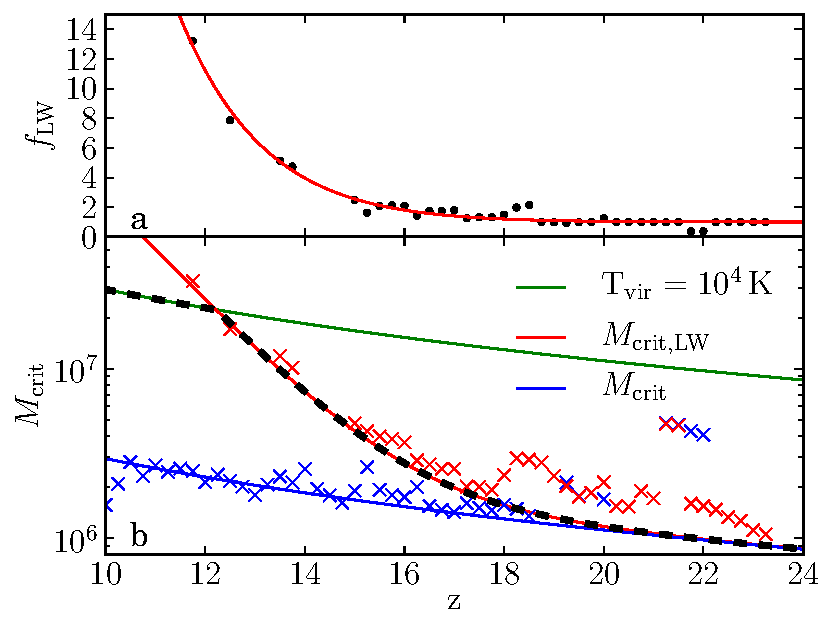
\includegraphics[width=\columnwidth]{lwFeedback}
   \caption{a) the factor $f_{\textsc{lw}}$ by which
     LW feedback increases the critical mass for star formation;
     points show the results of the simulation, the red line our fit.
     b) The critical mass for star formation in both simulations.
     Blue crosses mark the critical mass for star formation in the
     absence of LW feedback, red crosses in its presence.  The blue
     line shows the best fit critical mass from \RefEq{mcriteq}, given
     by a temperature of 2200 K; the red line the critical mass from
     \RefEq{mcritlweq} for LW feedback using the fit for
     $f_{\textsc{lw}}$ given in \RefEq{flweq}.  The green line marks
     the halo mass corresponding to a virial temperature of $10^4\,$K,
     and the black dashed line represents the critical mass employed,
     accounting for atomic cooling in halos with virial temperatures
     above $10^4\,$K.}
   \label{lwFeedback}
 \end{center}
\end{figure}

We will describe our radiative feedback simulations in detail
elsewhere, and present only a brief summary here.  We employ a set of
two cosmological simulations using a modified version of the
$N$-Body/TreePM SPH code GADGET \citep{Springel2005,Springeletal2001}
to gauge the effects of LW feedback on the PISN rate. These
simulations, carried out in a box of size $3.125 \,h^{-1}$ comoving
Mpc and starting from a redshift of $z=127$, were performed to
investigate the formation of the first dwarf galaxies in $10^9$\msun
halos at $z=10$. In order to obtain high resolution in the halo
containing the first galaxy while retaining information about
structure on large scales, a zoomed simulation technique was used,
with the highest resolution dark matter (gas) particles having a mass
of 2350 (484)\msun. This allows halos with masses $\gtrsim 2
\times 10^5$\msun, to be resolved with $\gtrsim 100$ dark
matter particles.

The first of the simulations we employ is similar to simulation \textit{Z4} 
presented in \citet{PawlikMilosavljevicBromm2011}, and follows
the non-equilibrium chemistry and cooling of the primordial atomic and
molecular gas, including star formation but not the associated
feedback.  It thus provides a useful reference against which the
effects of LW feedback can be discussed. Here, gas particles were
turned stochastically into star particles at densities $n_{\mathrm H} >
500 \,{\mathrm cm}^{-3}$ on a dynamical time scale. Star particles were
considered simple stellar populations using the zero-metallicity
top-heavy IMF models from \citet{Schaerer2003}.  Henceforth this
simulation is referred to as Simulation A.

The second simulation employed here, which we refer to as Simulation
B, is identical to Simulation A except for the inclusion of LW
feedback.  Calculation of the feedback was carried out by considering
the contribution from both star particles and a uniform LW background.
The combined LW background is normalized to approximate the LW
background evolution shown in \citet{GreifBromm2006} in the optically
thin limit, but with the application of a self-shielding correction
\citep{Wolcott-GreenHaimanBryan2011}.


The efficiency of LW feedback, $\eta_{\textsc{lw}}$, can be expressed
as the ratio of the formation rate of minihalos at the critical mass
with LW feedback to that without:
\begin{equation}
  \eta_{\textsc{lw}}(z) = \frac{ \dot{n}_{+}(M_{\mathrm crit, \textsc{lw}},
    z) }{ \dot{n}_{+}(M_{\mathrm crit}, z)}.
\end{equation}
This requires determining the factor $f_{\textsc{lw}}(z)$ by which LW
feedback increases the critical mass for star formation.  We do this
by determining the critical mass required for stars to form in both
simulations, as traced by the lowest mass halo that is actively
forming stars for the first time.  The resulting critical mass in each
case is shown in \RefFig{lwFeedback}b; blue points denote the critical
mass in Simulation A, red points in Simulation B.  Without any
negative feedback, we expect stars to form when the halo reaches the
critical mass given in \RefEq{mcriteq}.  We find the that the resulting critical
mass in Simulation A is best fit by a critical virial temperature of
2200 K, as shown in \RefFig{lwFeedback}b.  Note that this includes the
effects of dynamical heating; gas in isolated halos would collapse and
form stars at lower masses.

Determining the critical mass for star formation in the LW feedback
simulation in the same manner as above, we can then determine
$f_{\textsc{lw}}$, shown in \RefFig{lwFeedback}a.  We find that
$f_{\textsc{lw}}$ is well fit by a functional form of
\begin{equation}
  \label{flweq}
  \begin{split}
 f_{\textsc{lw}}(z) = -6.23\times10^{-5} \;
 &\textrm{erf}[0.094 (z - 0.204)] \\
 &+ 6. 23\times10^{5},
 \end{split}
\end{equation}
for $z\geq10$, where ${\mathrm erf}(z)$ is the error function.
$M_{\mathrm crit, \textsc{lw}}$ is then given by
\begin{equation}
  \label{mcritlweq}
M_{\mathrm crit, \textsc{lw}} = f_{\textsc{lw}} \,M_{\mathrm crit},
\end{equation}
shown in \RefFig{lwFeedback}b.  When the virial temperature of the
halo reaches $10^4\,$K, cooling via atomic hydrogen becomes efficient
and molecular hydrogen becomes unimportant.  Once this threshold is
reached, LW feedback cannot further suppress star formation, and
$M_{\mathrm crit, \textsc{lw}}$ holds steady at a constant virial
temperature of $10^4\,$K.  This is reflected as an increase in the
formation rate of halos affected only by LW feedback, as the formation
rate of atomic cooling halos is increasing prior to $z=10$.  This
transition can be clearly seen in \RefFig{fbrate}, marked by a sudden
jump in the halo formation rate.  As ionizing photons cannot easily
escape the immediate vicinity of the star that produced them, their
impact on neighboring halos is small compared to that of LW photons at
the highest redshifts.  We thus set $\eta_{\mathrm rad} \simeq
\eta_{\textsc{lw}}$ for simplicity.  This approximation becomes
increasingly unphysical close to the epoch of reionization at
$z\sim10$.
\begin{figure}
 \begin{center}
   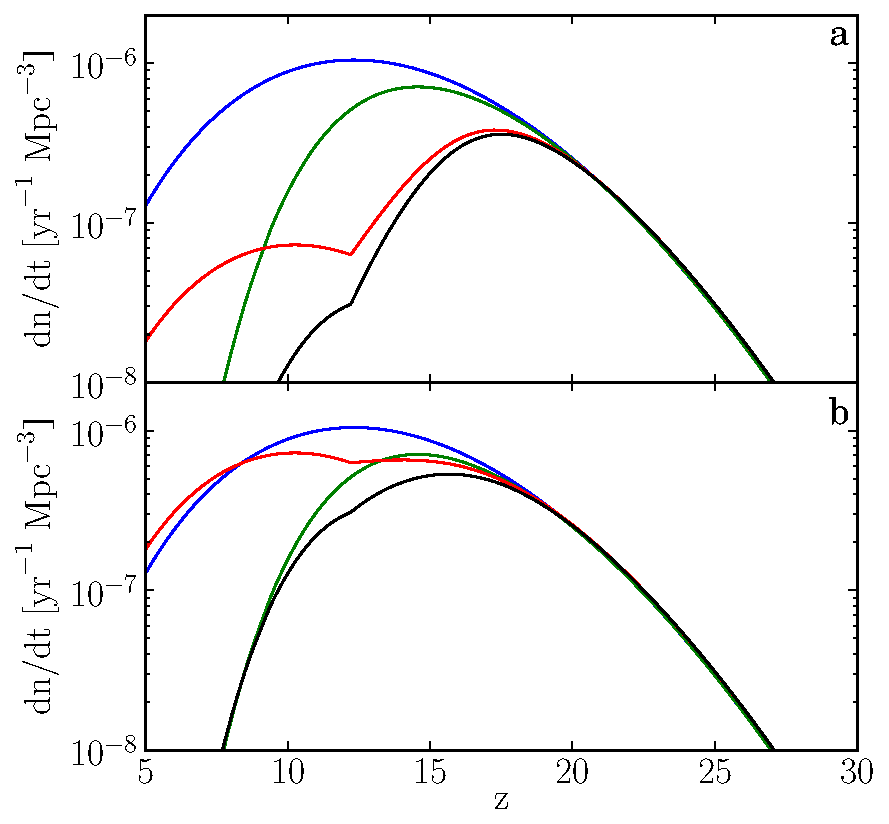
\includegraphics[width=\columnwidth]{feedbackRate}
   \caption{a) $\dot{n}_{\textsc{pisn}}$ in the upper limit of no
     feedback (blue), with chemical feedback (green), LW feedback
     (red) and the resulting PISN rate for the conservative (chemical
     plus LW) feedback case (black).  b) Same as (a), but for enhanced
     massive star formation.}
   \label{fbrate}
 \end{center}
\end{figure}


\subsubsection{Chemical Feedback}
The process of chemical enrichment is another crucial factor for
determining the PISN rate.  Gas that has been enriched beyond a
critical metallicity of $Z_{\mathrm crit} \sim 10^{-4}$\zsun will
no longer form Pop~III stars \citep{BrommKudritzkiLoeb2001,
  Schneideretal2002, BrommLoeb2003}, and hence no PISNe.  Chemical
feedback can thus be represented as the fraction of halos forming from
pristine gas at a given redshift.  Realistic three-dimensional
simulations of this process starting from cosmological initial
conditions have become possible in the past decade, showing that
enrichment by Pop~III SNe, if they are highly energetic, proceeds very
inhomogeneously, enriching the IGM before penetrating into denser
regions \citep{Scannapiecoetal2005, Greifetal2007,
  TornatoreFerraraSchneider2007,WiseAbel2008, Maioetal2010}.

In modeling $\eta_{\mathrm chem}$, we use the results of
\citet{FurlanettoLoeb2005}.  Their semi-analytic treatment of SN winds
utilizes the \citet{Sedov1959} solution for an explosion expanding
into a uniform medium and yields a probability function $P_{\mathrm
  pristine}(z)$ that the gas in a newly formed halo is pristine.  This
is plotted in Figure 2 of their paper for various strengths of
chemical feedback.  We identify this quantity as the fraction of newly
collapsed halos that have been polluted with metals, $\eta_{\mathrm
  chem}$.  Given the recent detection of pristine gas at $z = 3$ by
\citet{FumagalliOMearaProchaska2011}, we choose the weakest feedback
scenario presented by \citet{FurlanettoLoeb2005} among the scenarios
that incorporate a clustering of sources. The resulting PISN rate is
given by the green line in \RefFig{fbrate}.

\subsection{Enhanced Massive Star Formation}
Gas cooling and subsequent star formation in halos affected by LW
feedback can be delayed until nearly an order of magnitude more gas is
available for star formation (\RefFig{lwFeedback}). This increases the
likelihood that multiple massive stars form per halo, offseting the
negative effects of LW radiation considered above.  We quantify this
by positing that the number of PISNe produced per halo at redshift $z$
is given by the ratio of the critical mass in the presence of LW
feedback $M_{\mathrm crit, \textsc{lw}}$ to the critical mass in the
no-feedback case $M_{\mathrm crit}$.  For example, at $z=17$, $M_{\mathrm
  crit, \textsc{lw}} / M_{\mathrm crit} \approx 1.4$, so for every 10
pristine halos that form, 14 PISNe are produced.  In this case the
PISN rate is modified such that
\begin{equation}
\dot{n}_{\textsc{pisn}}(z) = \frac{M_{\mathrm crit, \textsc{lw}}(z)}{M_{\mathrm crit}(z)} \;
\eta_{\mathrm chem}(z) \; \eta_{\mathrm rad}(z) \; \dot{n}_{+}(z).
\label{pisnrate2}
\end{equation}
The resulting enhanced PISN rate can be seen in \RefFig{fbrate}b.  In
contrast to the conservative feedback case, the net effect of LW
feedback is much less significant here, with chemical feedback
controlling the final PISN rate.

\subsection{The Observable Rate}
\begin{figure}
 \begin{center}
   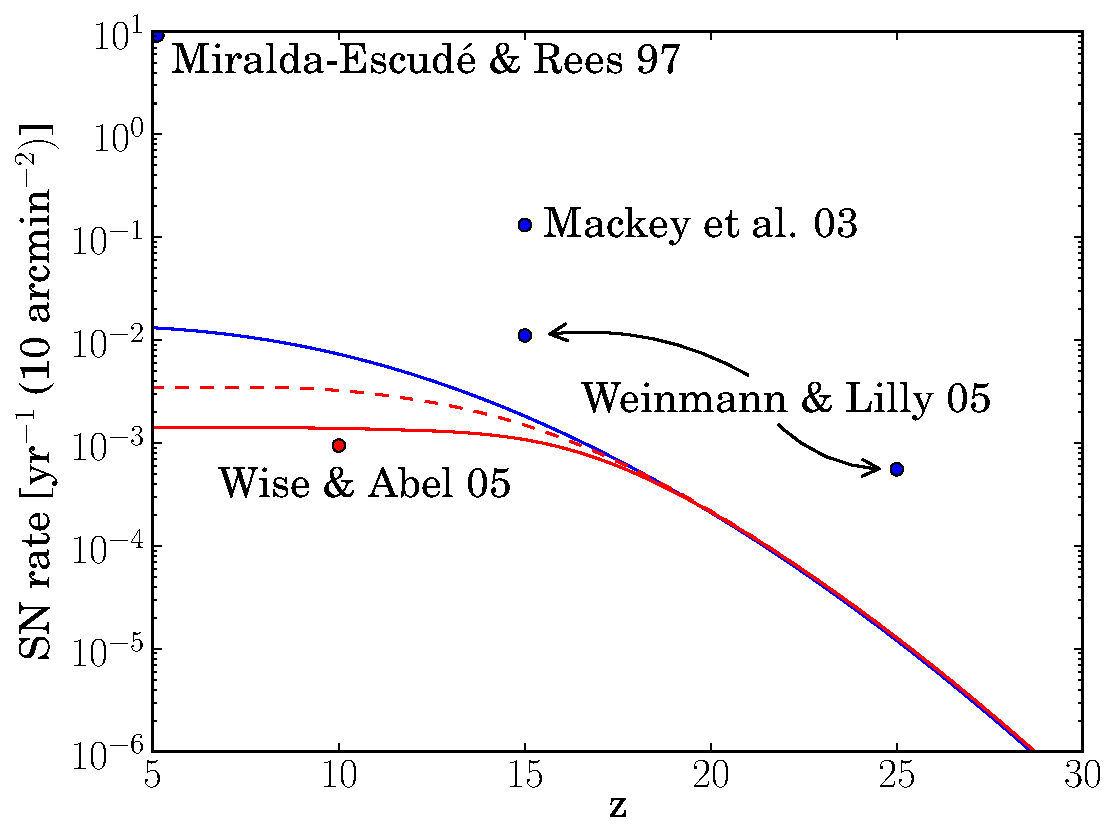
\includegraphics[width=\columnwidth]{observableRate}
   \caption{The observable PISN rates in number per year
     per JWST field of view above a given redshift in the upper limit
     of no feedback (blue line), in the conservative feedback case
     (solid red line), and the enhanced star formation case (dashed
     red line).  The rates calculated by
     \citet{Miralda-EscudeRees1997}, \citet{MackeyBrommHernquist2003},
     \citet{WeinmannLilly2005} and \citet{WiseAbel2005} are also shown
     for reference. Red points account for feedback; blue points do
     not.}
   \label{obsrate}
 \end{center}
\end{figure}
The observed PISN rate per unit time per unit redshift per unit solid
angle is given by
\begin{equation}
  \begin{split}
    \frac{dN}{dt_{\mathrm obs}\,dz\,d\Omega} &= \frac{dN}{dt_{\mathrm
        obs}\,dV} \, \frac{dV}{dz d\Omega}
    \\ &=\frac{1}{(1+z)}\frac{dN}{dt_{\mathrm em}\,dV} \;r^2
    \frac{dr}{dz}.
 \end{split}
\end{equation}
Cosmological time dilation between $t_{\mathrm obs}$ and $t_{\mathrm em}$ is
accounted for by the $(1+z)$ in the denominator; $dV$ is the
comoving volume element and $r(z)$ is the comoving distance to
redshift $z$ given by
\begin{equation}
r(z) = \frac{c}{H_0}\int_0^z \frac{dz'}{\sqrt{\Omega_{\mathrm m} (1+z')^3 +
    \Omega_{\Lambda}}},
\end{equation}
where $c/H_0$ is the Hubble distance.  With the assumptions outlined
above, we estimate the PISN rate in events per year per comoving
Mpc$^3$ in the source rest frame:
\begin{equation}
\frac{dN}{dt_{\mathrm em}\,dV} = \dot{n}_{\textsc{pisn}}(z).
\end{equation}
These results---shown in \RefFig{obsrate}---are in reasonable
agreement with previous work; our no-feedback limit of one PISN per
minihalo is somewhat more conservative than that employed by
\citet{WeinmannLilly2005}, but in general agreement.  Likewise, our
conservative feedback rate is in good agreement with the rate found by
\citet{WiseAbel2005}, which also accounted for feedback.  The
discrepancy with the remaining rates can be attributed to the fact
that \citet{MackeyBrommHernquist2003} employed an optimistic star
formation efficiency of $\eta_*=0.10$, while
\citet{Miralda-EscudeRees1997} performed a rough estimate of the
all-sky supernova rate based on the observed metallicity of the
IGM. This estimate of course includes Population~I and II supernovae in
addition to PISNe, and is included only for reference.


\section{JWST Observability}
\label{JWSTobs}
While PISN explosions are predicted to be extremely energetic, the
highest redshift events will still be unobservable, and those at lower
redshifts will be above the detection limits of the JWST for only a
fraction of their lifetimes. To determine the observability of these
explosions we must consider both how bright they will be at a given
redshift and how long they will remain visible.  To span the
uncertainties arising from variation in the progenitors of PISNe we
consider a set of four models from \citet{KasenWoosleyHeger2011},
namely their R250, B200, R175 and He100 models.  R250 and R175 are red
supergiants of 250\msun and 175\msun, respectively, spanning the mass
range of succesful explosions.  We also consider a more compact
200\msun blue supergiant (B200) and a 100\msun bare helium core
(He100).  All models considered here die as PISNe, with explosion
energies ranging from $7\times10^{52}$ ergs (R250) to $2\times10^{52}$
ergs (R175).  The late-time luminosity is powered by the decay of
$^{56}$Ni produced during the explosion.  40\msun of $^{56}$Ni are
produced in the R250 model, while only 5, 2 and 0.7\msun are produced
in He100, B200 and R175, respectively.

Bare helium cores, such as the He100 model, are of particular interest
in light of recent work finding that rapidly rotating stars can
encounter the pair-production instability in progenitors with masses
as low as 65\msun \citep{ChatzopoulosWheeler2012,
  YoonDierksLanger2012}. Combined with recent work finding that
Pop~III stars are both less massive and more rapidly rotating than
previously thought \citep{StacyGreifBromm2010, StacyBrommLoeb2011,
  StacyGreifBromm2012, Clarketal2011b, Greifetal2011, Greifetal2012},
the explosion of a rapidly rotating helium core formed by homogeneous
evolution represents an intriguing possibility.

We first describe our technique for fitting a blackbody to these four
PISN models before considering their visibility with the JWST. We then
estimate the total observable number in each case and for each
feedback prescription.  Finally, we briefly discuss the challenges
involved in actually identifying PISNe as such.

\subsection{A Simple Lightcurve Model}
In order to determine how long a PISN will be visible we must model
the source spectrum. Given the large mass involved, the ejecta will
remain optically thick until late times, so we make the reasonable
assumption that the PISN emits as a blackbody for the majority of its
visible lifetime.  Using the U, B, V, R, I, J, H, and K absolute
magnitude light curves presented in \citet{KasenWoosleyHeger2011}, we
perform a least-squares fit to find the combination of temperature $T$
and radius $R_{\textsc{sn}}$ that best matches the broadband
magnitudes at each point in time. This is done with the assumption
that the specific luminosity of the PISN $L_{\textsc{sn}, \lambda}$ at
wavelength $\lambda$ is given by
\begin{equation}
L_{\textsc{sn},\lambda} = 4\pi^2 R_{\textsc{sn}}^2 B_{\lambda}(T),
%= 4\pi R_{\textsc{sn}}^2 F_{\lambda} 
\end{equation}
where $B_{\lambda}$ is the Planck function. The resulting fits for the
evolution of the temperature and radius of the PISN models are shown in
\RefFig{bbmodels}.
\begin{figure}
  \begin{center}
    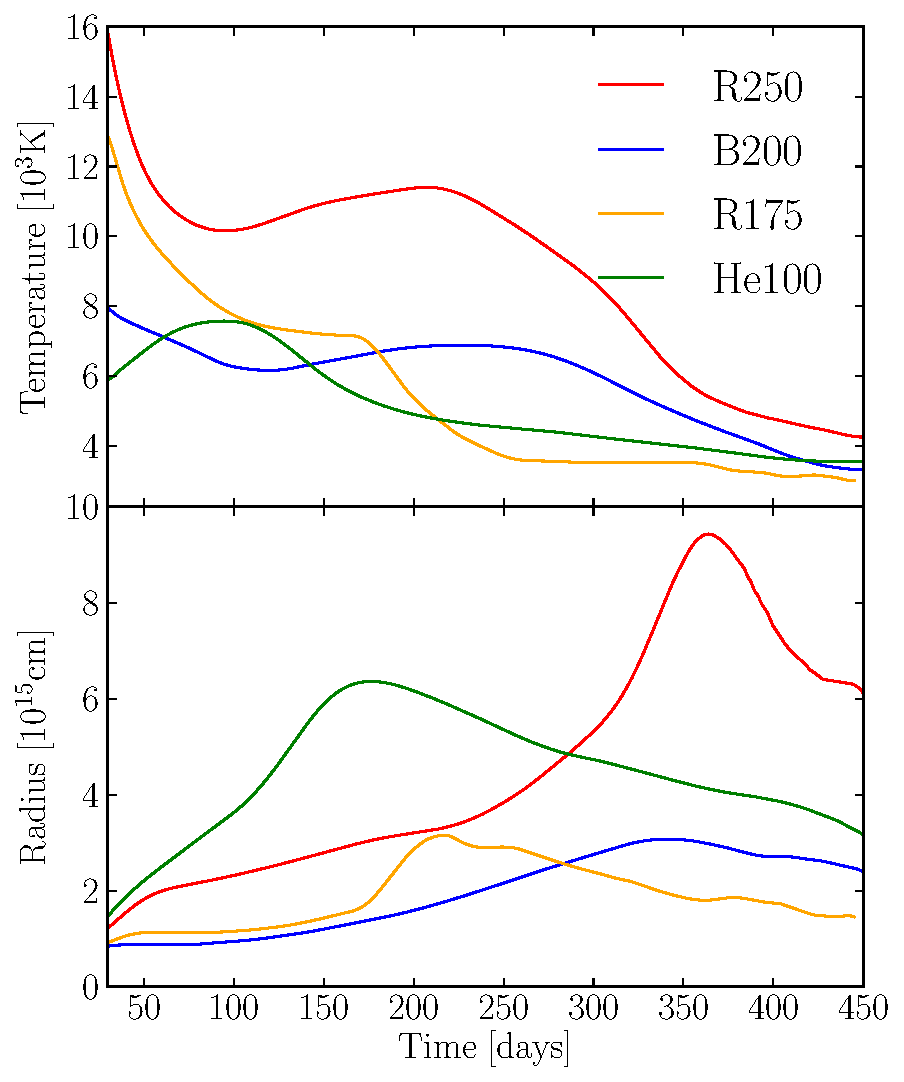
\includegraphics[width=\columnwidth]{bbmodels}
    \caption{The temperature and radius of our blackbody
      fits as a function of source frame time since the explosion
      for models R250, B200, R175 and He100.  The secondary rise in
      temperature seen in R250 and B200 is caused by the decay of
      $^{56}$Ni reheating the ejecta at late times.  Note also that the
      apparent radii begin to decrease again at late times; this can
      be interpreted as the photosphere receding into the ejecta as
      the material cools.}
    \label{bbmodels}
  \end{center}
\end{figure}
Note that our blackbody assumption breaks down at late times when the
photosphere begins to recede into the ejecta.  This is manifested as
an apparent decrease in the radius of the PISN remnant.

\begin{figure}
 \begin{center}
   \resizebox{15cm}{12cm}
   {\unitlength1cm
     \begin{picture}(15,12)
       \put(0,6){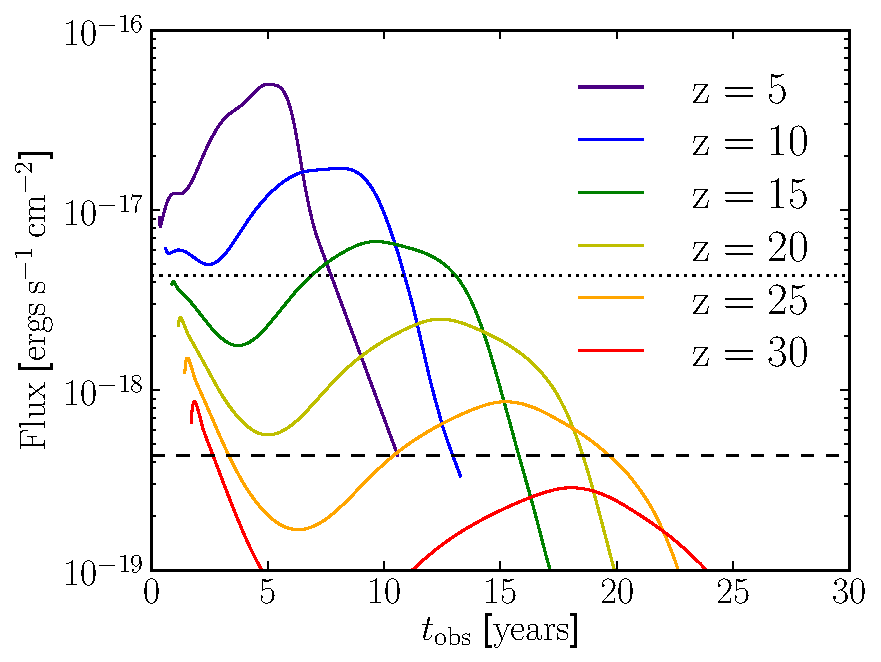
\includegraphics[width=7.5cm,height=6cm]{R250flux_F444W}}
       \put(7.5,6){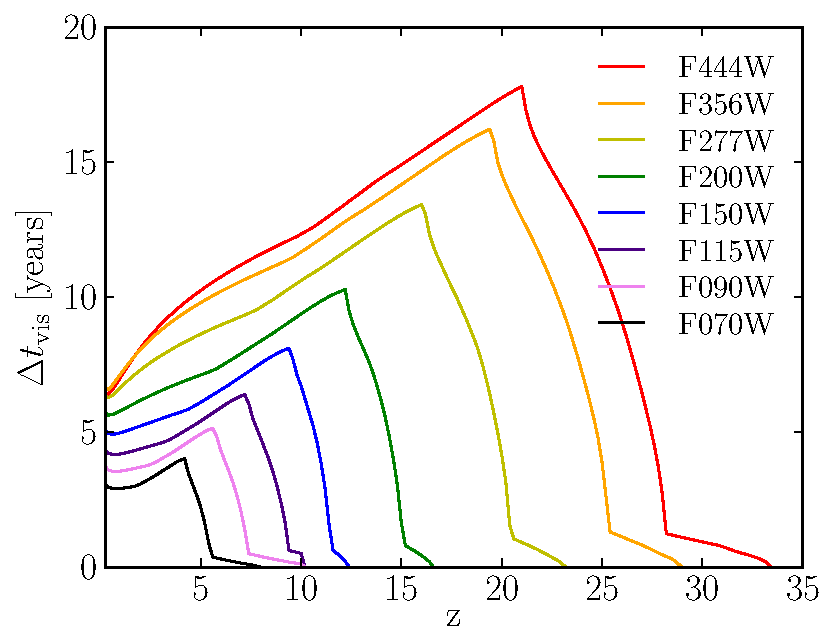
\includegraphics[width=7.5cm,height=6cm]{R250_t6}}
       \put(0,0){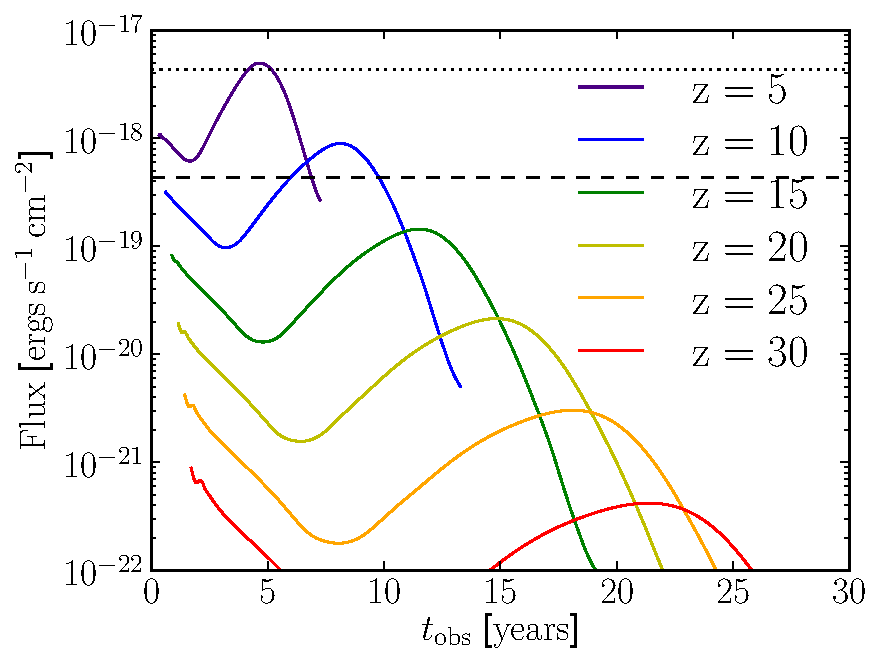
\includegraphics[width=7.5cm,height=6cm]{B200flux_F444W}}
       \put(7.5,0){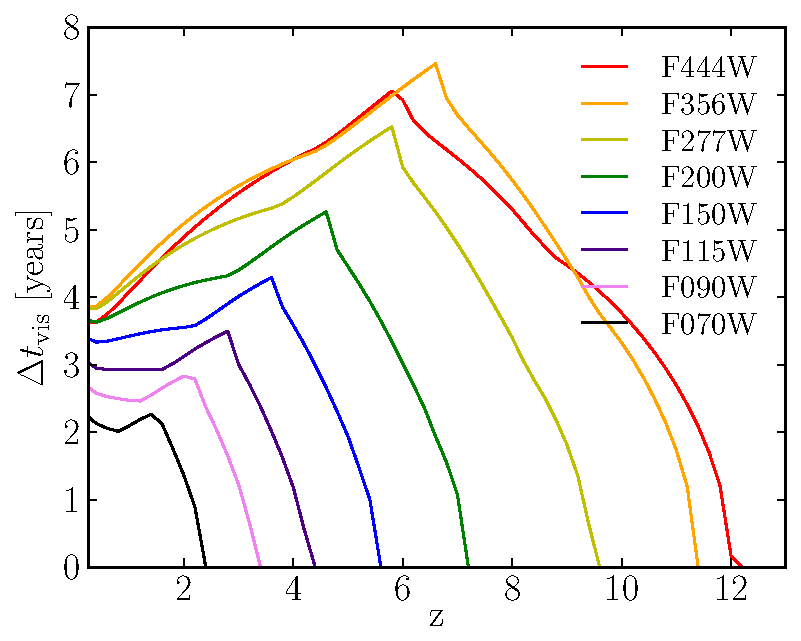
\includegraphics[width=7.5cm,height=6cm]{B200_t6}}
  \end{picture}}
\caption{Left: Lightcurves for the
  \citet{KasenWoosleyHeger2011} R250 (top) and B200 (bottom) models as
  they would be observed by JWST's F444W NIRCam filter at $z = 5, 10,
  15, 20, 25 \:{\mathrm and}\: 30$. The flux limits for a $10^6\,$s
  (dashed line) and $10^4\,$s (dotted line) exposure are shown for
  reference.  Right: The visibility time $\Delta t_{\mathrm vis}$ in years
  for R250 (top) and B200 (bottom) as a function of redshift for each
  of the NIRcam wide filters. Note that the axes are scaled
  independently.  Similar plots for models He100 and R175 are included
  in the appendix.}
   \label{visibility}
 \end{center}
\end{figure} 

With this information we can then calculate the specific flux
$F_{\lambda, \mathrm em}$ in the rest frame and|accounting for redshift
and cosmological dimming|in the observer's frame for a source at
redshift $z$:
\begin{equation}
F_{\lambda, \mathrm obs}(T,R_{\textsc{sn}}, z) = \pi
\left[\frac{R_{\textsc{sn}}}{D_L(z)}\right]^2
\frac{B_{\lambda'}(T)}{1+z}.
\end{equation}
Here $\lambda' = \lambda/(1+z)$ accounts for redshifting, and the
luminosity distance $D_L = (1+z) r(z)$ accounts for cosmological
dimming.  Convolving this spectrum with a filter function
$\phi_\textsc{x}(\lambda)$ yields the observable flux in filter~X:
\begin{equation}
F_{\mathrm obs, \textsc{x}} = \int_{0}^{\infty} \phi_\textsc{x}(\lambda)
F_{\lambda, \mathrm obs}(T,R_{\textsc{sn}}, z) d\lambda.
\end{equation}

\subsection{Visibility}
The NIRCam instrument on the JWST will observe the early universe
through a number of narrow, medium-width, and wide
filters\footnote{http://www.stsci.edu/jwst/instruments/nircam/instrument-design/filters}.
The widest, longest-wavelength filter, F444W, will observe from 3.3 to
5.6 $\mu$m with a sensitivity limit of 24.5 nJy required for a
$10\sigma$ detection in $10^4\,$seconds \citep{Gardneretal2006}. Shown
in the left-hand column of \RefFig{visibility} is the observable flux
as it would appear in the F444W NIRCam filter at various redshifts for
the most and least easily observable models, R250 and B200,
respectively. See \RefFig{observability} for why these two were
chosen; models He100 and R175 can be found in the appendix.  The flux
limits for the filter of $4.4 \times 10^{-19}$ erg s$^{-1}$ cm$^{-2}$
for a $10^6\,$s exposure and $4.4 \times 10^{-18}$ erg s$^{-1}$
cm$^{-2}$ for a $10^4\,$s exposure are also shown for reference.  We
see that the brightest explosions (R250) would be visible to beyond
$z\sim25$, but are never so bright as to be detectable with current
generation telescopes.  This is consistent with the non-detection by
\citet{Frostetal2009} in a search of the \textit{Spitzer}/IRAC Dark Field
for possible Pop~III PISN candidates.

To account for absorption of flux by neutral hydrogen along the line
of sight we implement a simple model of instant reionization at
$z=10$.  For sources above this redshift, we assume no flux is
observed shortward of the rest frame Ly$\alpha$ line.  This is not
relevant for the F444W NIRcam filter as Ly$\alpha$ does not redshift
into the filter until $z\sim40$, when the lightcurve is already far
below even the $10^6\,$s sensitivity limit.  It does however have an
effect, albeit a small one, on the F115W and F090W filters.

At low redshifts the duration of the lightcurve presented in
\citet{KasenWoosleyHeger2011} is not quite long enough for the
observed flux to reach the sensitivity limit; we extend it to the
limit by extrapolating assuming a power-law scaling.  The visible time
$\Delta t_{\mathrm vis}$ is then simply given by the time the lightcurve
is above the filter sensitivity limit.  Shown in \RefFig{visibility}
are the visibility times as a function of redshift for each of the
NIRcam filters.  

\begin{figure}
 \begin{center}
   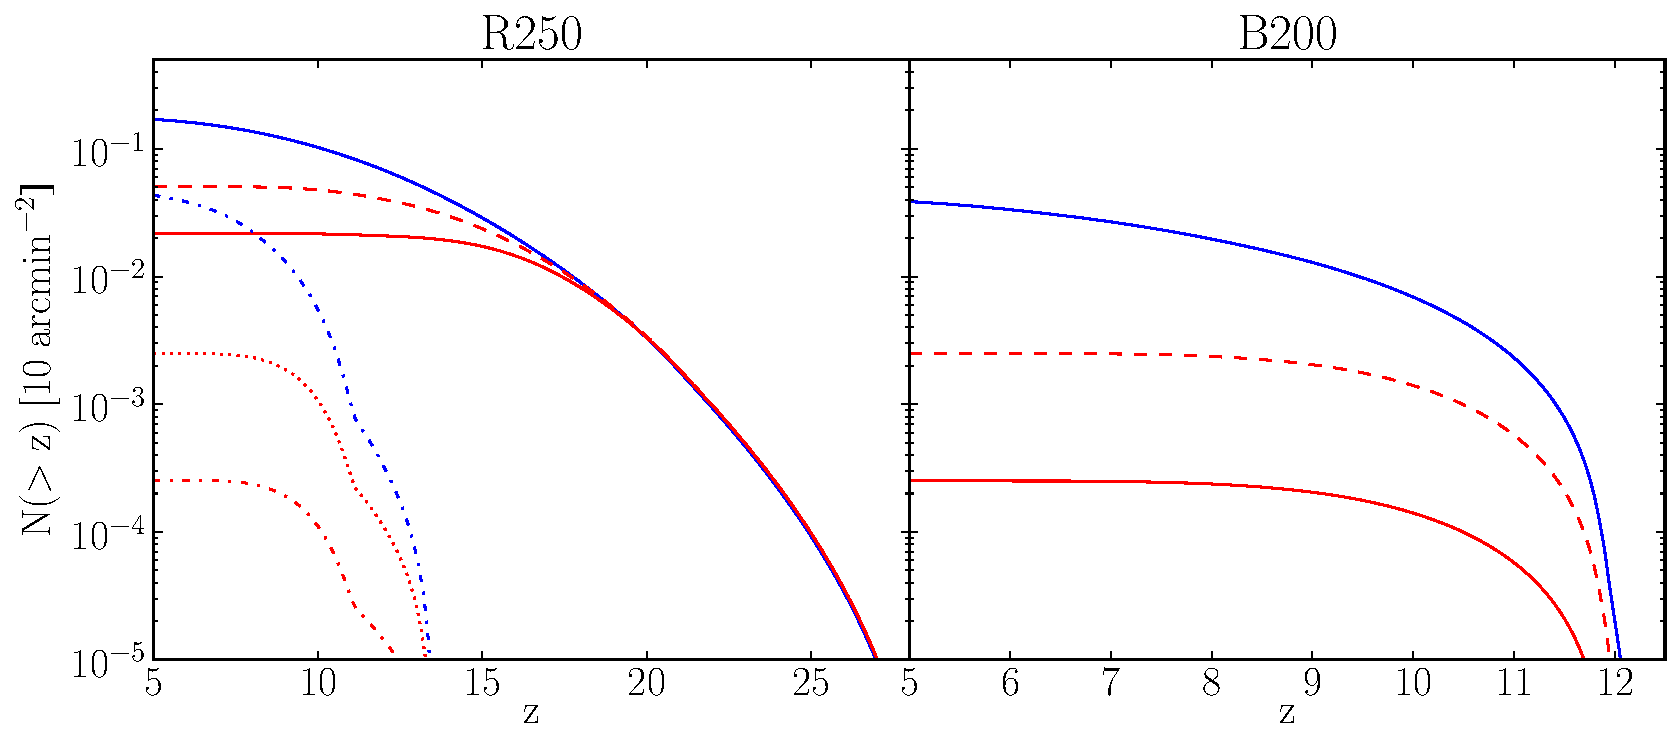
\includegraphics[width=\columnwidth]{observableNumber}
   \caption{Upper and lower limits for the number of
     PISNe per JWST FoV above redshift $z$ with different feedback
     prescriptions. The observable numbers for a $10^6\,$s exposure
     assuming the R250 model are shown on the left; the B200 model is
     employed on the right. Solid blue lines show an upper limit to
     the observable number in the case of no feedback, solid red lines
     an estimate for the observable number in our conservative
     feedback scenario, and dashed red lines the number in the
     enhanced star formation case. Note that the x-axis is scaled
     independently in each panel.  Also shown in the R250 panel are
     the observable numbers for a $10^4\,$s exposure for the
     no-feedback (dot-dashed blue), conservative feedback (dot-dashed
     red), and enhanced star formation (dotted red) scenarios. The
     B200 model is not visible above $z=5$ in a $10^4\,$s exposure.}
   \label{obsnumber}
 \end{center}
\end{figure} 
\subsection{The Observable Number}
 With this estimate for $\Delta t_{\mathrm vis}$, we may finally calculate
 the observable number of PISNe on the sky, given by the product of
 the PISN rate at $z$, as seen in the observer frame, and the time a
 PISN at $z$ is visible, $\Delta t_{\mathrm vis}$. This yields an estimate
 for the number of PISNe visible on the sky at any given time per unit
 redshift per unit solid angle:
\begin{equation} 
\frac{dN}{dz\,d\Omega} \simeq \frac{dN}{dt_{\mathrm
    obs}\,dz\,d\Omega}\,\Delta t_{\mathrm vis}.
\end{equation}
\RefFig{obsnumber} shows the number of PISNe per JWST field of view
(FoV) above redshift $z$ in a $10^6\,$s exposure for all three
feedback cases for models R250 and B200. Models He100 and R175 can be
found in the appendix.  For the R250 model the results for a $10^4\,$s
exposure are also included; B200 is not visible at high redshifts in a
$10^4\,$s exposure.

In the optimistic case of an R250-type PISN with no feedback we expect
\about0.2 PISNe per JWST FoV for a $10^6\,$s exposure.  In the most
pessimistic case of a B200-type PISN with strong negative feedback
this number drops to \about2.5$\,\times10^{-4}$ per FoV.  The actual
number detected by the JWST will most likely lie somewhere within this
range. Given this, we conclude that a single deep pencil-beam survey
is unadvisable for detecting PISNe, as there aren't enough in a given
field to ensure a detection, even in the most optimistic upper limit.
This suggests that a mosaic search, covering a larger area with shorter
exposure times, may be the best approach to ensure finding a Pop~III
PISN.

\subsection{PISN Identification}
The exceedingly long duration of their lightcurves poses a serious
challenge for identifying PISNe.  When combined with the cosmological
time dilation factors involved, PISN lightcurves can last for decades;
the highest redshift events will last longer than the projected
mission lifetime for the JWST, making the detection of PISNe by
searching for transients difficult at best.  However, a multi-year
campaign might be able to detect photometric variations; for example,
the He100 model would appear to decline in brightness by \about0.3
magnitudes per year at redshift $z=10$
\citep{KasenWoosleyHeger2011}. Additionally, PISN colors become redder
over time as the photosphere receeds into the ejecta and metal line
blanketing suppresses flux in the bluer bands.  While likely
insufficient to unambiguously identify PISNe, this could be useful in
selecting candidates for spectroscopic follow-up.

While the peak bolometric luminosities and spectra of PISNe resemble
those of typical Type Ia and Type II supernovae
\citep{JoggerstWhalen2011, KasenWoosleyHeger2011}, relatively little
mixing occurs during the explosion \citep{JoggerstWhalen2011,
  ChenHegerAlmgren2011}.  As a result, PISNe mostly retain their
onion-layer structure during the explosion, and metal lines do not
appear in the spectrum until late times when the photosphere has
receeded deep into the ejecta.  Some lighter elements may appear, but
the early spectrum of a PISN will be devoid of Si, Ni and Fe lines
\citep{JoggerstWhalen2011}. This may provide the spectroscopic
signature needed to identify PISNe.

\section{Discussion and Conclusions}
\label{conclusions} 
\begin{figure}
\begin{center}
  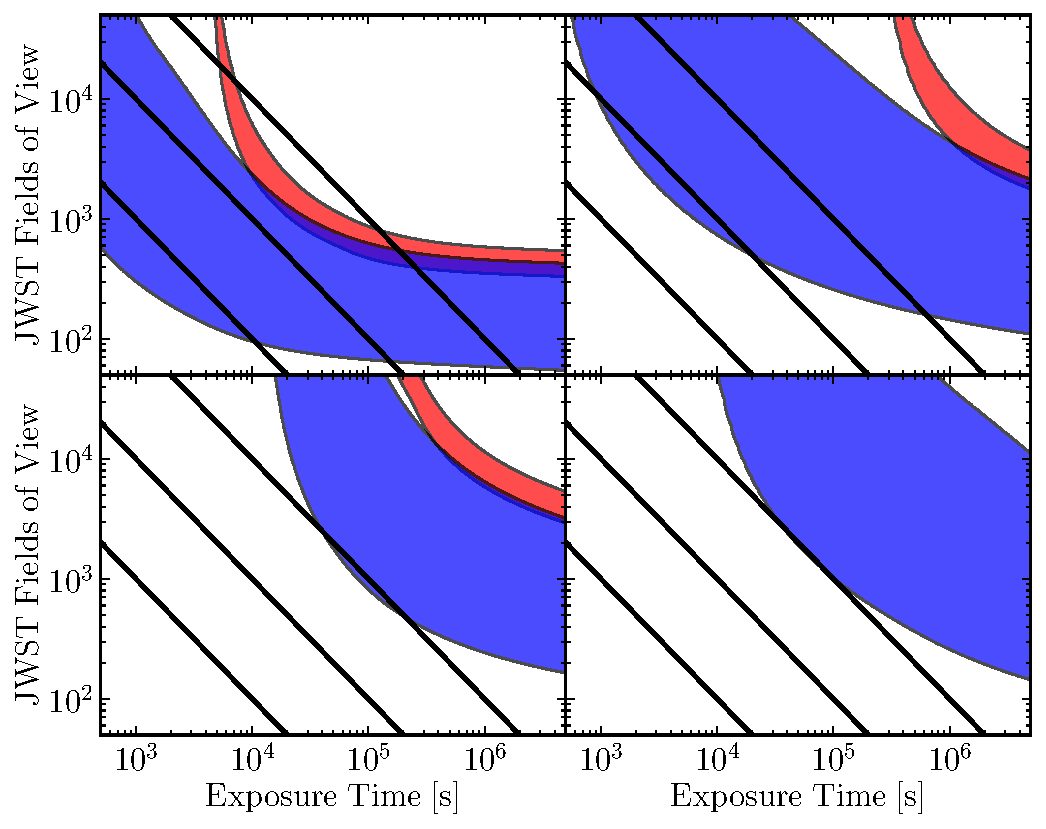
\includegraphics[width=\columnwidth]{observability}
  \caption{The observability of the R250, He100, B200,
    and R175 models (clockwise from upper left) from
    \citet{KasenWoosleyHeger2011} using the JWST's NIRcam F444W
    filter. Shown is the possible range for the number of JWST FoVs
    required to detect 10 sources as a function of exposure time. The
    blue range is for all PISNe, and the red for PISNe
    from $z>15$.  The lower boundaries correspond to the
    no-feedback upper limit to the PISN rate and the upper boundaries to
    the conservative feedback rate.  From left to right, the black
    lines represent the number of pointings possible in a total of
    $10^6$, $10^7$, and $10^8\,$s for a given exposure time.}
  \label{observability}
\end{center}
\end{figure}

In this work, we have examined the source density of PISNe from
Pop~III stars and considered their detectability with the JWST. We
conclude that the limiting factor in detecting PISNe will be the
scarcity of sources rather than their faintness, in agreement with the
conclusions of \citet{WeinmannLilly2005}. The brightest PISNe should
be readily detectable with the longest wavelength NIRcam filters out
to $z\sim25$; the problem is the overall scarcity of sources.

 We have derived an estimate for the observable PISN rate, finding an
 upper limit of just over 0.01 PISNe per year per JWST FoV in the case
 of negligible chemical and radiative feedback. We also find that the
 inclusion of feedback can reduce the PISN rate by an order of
 magnitude, to \about0.001 per FoV. Accounting for the possibility of
 enhanced massive star formation in halos affected by LW radiation improves
 this rate slightly, to \about0.003 per FoV.  The derived PISN rate
 then allows us to place an upper limit on the observable number of
 PISNe in a $10^6\,$s exposure of \about0.2 PISNe per JWST FoV in the
 no-feedback case. The most pessimistic case of a B200-type PISN with
 strong negative feedback reduces this number to
 \about2.5$\,\times10^{-4}$ per FoV, or one PISN per 4000 JWST fields
 of view.

 The long duration of PISN lightcurves imply that spectroscopic
 follow-up of PISNe will likely be of great importance. PISN
 lightcurves can last for decades when combined with the cosmological
 time dilation factors at high redshifts, making the detection of
 PISNe by looking for transients untenable.  However, a multi-year
 campaign could identify candidates photometrically, and the lack of
 metal lines in the spectrum at early times could provide a
 spectroscopic signature for identification.

We find that the main obstacle to observing PISNe is the paucity of
sources.  Beyond a moderate exposure time of a few times $10^4\,$s,
the observability of bright PISNe is not a strong function of exposure
time and is instead controlled by the source density; this is evident
from \RefFig{observability}, where we have shown the number of JWST
FoVs required to detect 10 PISNe (blue) as a function of exposure time
for each of our PISN models.  The upper boundaries correspond to our
conservative estimate for the PISN rate in the presence of feedback,
and the lower boundaries to the estimated rate without feedback. We can
see that the decrease in the required number of JWST pointings slows
considerably beyond \about10$^5\,$s, hence a deep pencil-beam survey
would not be advisable in searching for PISNe. Even for only
high-redshift sources ($z>15$; red) the dependence on exposure time is
still minimal, being controlled by the lack of sources once the
required imaging depth is reached.

\begin{figure}
\begin{center}
  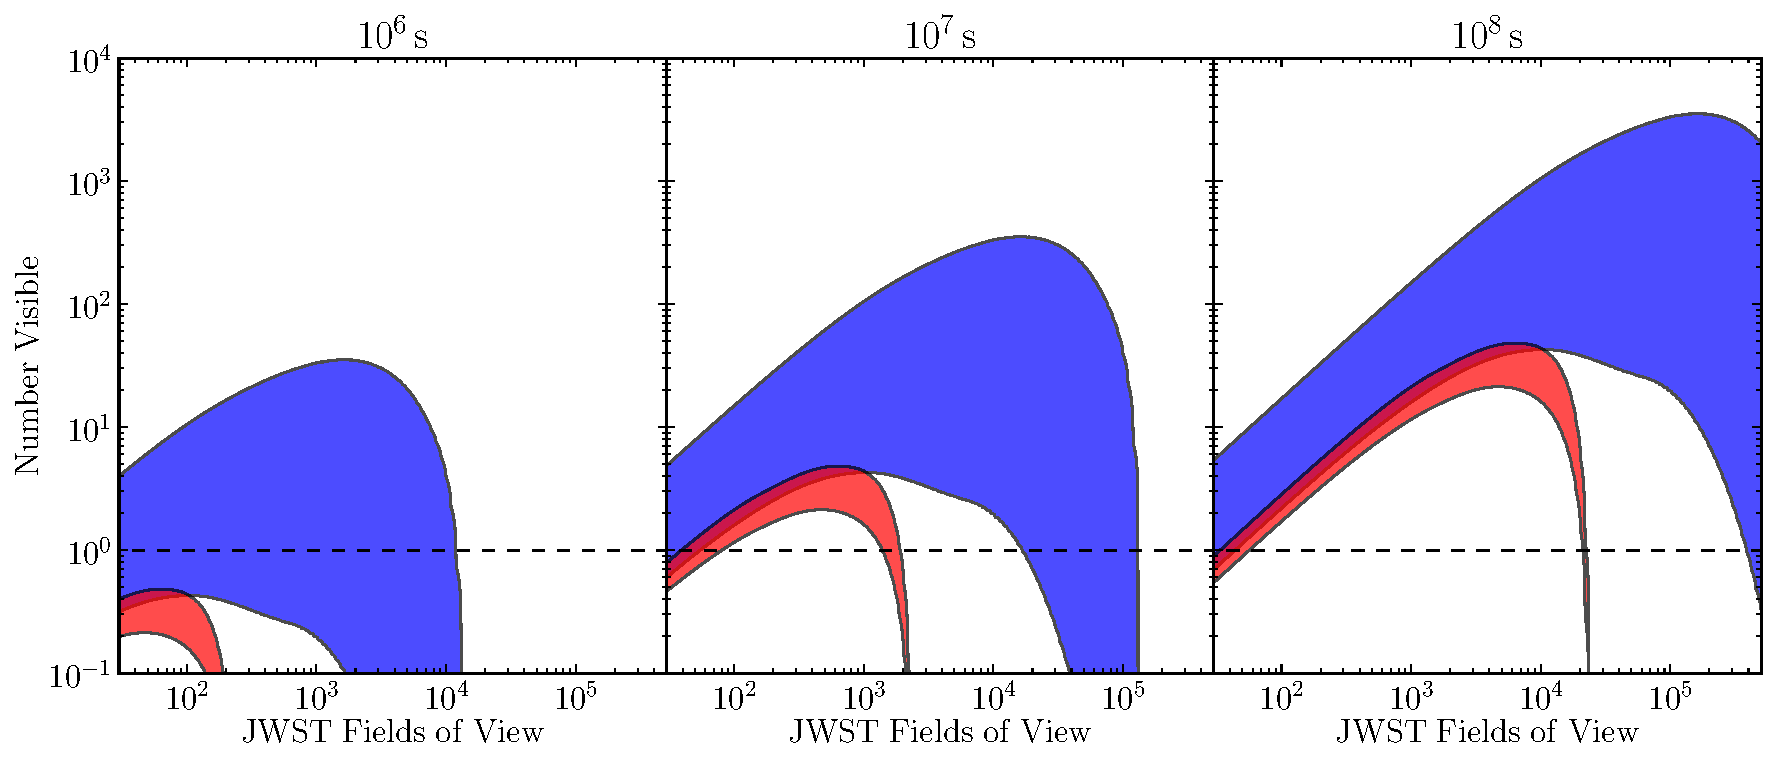
\includegraphics[width=\columnwidth]{area_observability_R250}
  \caption{The total number of PISNe observable with a
    campaign of $10^6$, $10^7$ and $10^8\,$s (from left to right) as a
    function of survey area for the R250 PISN model.  In each case,
    the total campaign time is apportioned equally over the total
    survey area to determine the exposure time for individual
    pointings.  The blue region represents all PISNe, the red only
    PISNe from $z>15$.  Upper boundaries correspond to the no-feedback
    upper limit to the PISN rate and lower boundaries to the
    conservative feedback case. For reference we mark the case of only
    one PISN visible (dashed line).}
 \label{area_obsR250}
\end{center}
\end{figure}  
Of particular interest in \RefFig{observability} are the black lines
representing the total number of pointings possible in $10^6$, $10^7$,
and $10^8\,$s for a given exposure time and their location relative to
the observability ranges in blue and red.  $10^6\,$s is approximately
the limit of what would be possible with a dedicated deep-field
campaign; $10^7\,$s is the limit of the observations the JWST could
make in a year assuming NIRCam is in use one third of the time;
$10^8\,$s (\about10 years) is the projected mission lifetime. 

While the detection of a PISN from a `first' star at very high
redshifts would be exciting and is in fact possible given the
detection limits of the JWST, the scarcity of sources at these
redshifts means that such a detection would be highly contingent on
serendipity. Even in the most optimistic case, with all available
minihalos producing an R250-type PISN, the observability range for
such events lies well above what is possible even in a full year of
observations, though a few may be detected over the lifetime of the
telescope.  The detection of a PISN at lower redshifts appears to be
more realistic.  As the faintest PISNe (R175 and B200) are effectively
unobservable, PISN searches should focus on looking for PISNe similar
to the R250 and He100 models.  In this case, the strategy with the
highest likelihood of detection will be a mosaic survey of many
moderately deep exposures.  This is clear from \RefFig{area_obsR250},
where we show the number of PISNe that will be observable with the
JWST in observing campaigns totalling $10^6$, $10^7$ and $10^8\,$s for
the R250 PISN model. The exposure time for each pointing varies with
the total area covered by the survey in order to keep the total
observing time constant.  Upper boundaries correspond to the number
visible in the no-feedback case, lower boundaries to the conservative
feedback case. As in \RefFig{observability}, the blue region shows the
observable number from all redshifts, the red region only those from
$z>15$.  We see that the observable number increases until the
resulting exposure time is no longer sufficient to detect PISNe.  The
optimal search strategy then will be to cover as large an area as
possible, going only as deep as necessary, possibly in a similar
manner to the ongoing Brightest of Reionizing Galaxies survey with the
\textit{Hubble Space Telescope} \citep{Trentietal2011, Bradleyetal2012}.

\chapter{A pandas-based Framework for Analyzing GADGET Simulation Data}

\section{Introduction}
\label{sec:intro}

In the past decade, astrophysical simulations have increased dramatically in both scale and sophistication, and the typical size of the datasets produced has grown accordingly.  
However, the software tools for analyzing such datasets have not kept pace, such that one of the primary barriers to exploratory investigation is simply manipulating the data.  
This problem is particularly acute for users of the popular smoothed particle hydrodynamics (SPH) code \textsc{gadget} \citep{SpringelYoshidaWhite2001,Springel2005}.  
Both \textsc{gadget} and \textsc{gizmo} \citep{Hopkins2015}, which uses the same data storage format, are widely used to investigate a range of astrophysical problems; unfortunately this also leads to fractionation of the data storage format as each research group modifies the output to suit its needs.
This state of affairs has historically forced significant duplication of effort, with individual research groups separately developing their own unique analysis scripts to perform similar operations.

Fortunately, the issue of data management and analysis is not endemic to astronomy, and the resulting overlap with the needs of the broader scientific community and the industrial community at large provides a large pool of scientific software developers to tackle these common problems.
In recent years, this broader community has settled on python as its programming language of choice due to its efficacy as a `glue' language and the rapid speed of development it allows.  
This has led to the development of a robust scientific software ecosystem with packages for numerical data analysis like \code{numpy} \citep{VanderWaltColbertVaroquaux2011}, \code{scipy} \citep{JonesOliphantPeterson2001}, \code{pandas} \citep{McKinney2010}, and \code{scikit-image}; \code{matplotlib} \citep{Hunter2007} and \code{seaborn} for plotting; \code{scikit-learn} for machine learning, and statistics and modeling packages like \code{scikits-statsmodels}, \code{pymc}, and \code{emcee} \citep{Foreman-Mackeyetal2013}.

Python is quickly becoming the language of choice for astronomers as well, with the Astropy project \citep{Robitailleetal2013} and its affiliated packages providing a coordinated set of tools implementing the core astronomy-specific functionality needed by researchers. 
Additionally, the development of flexible python packages like \code{yt} \citep{Turketal2011} and \code{pynbody} \citep{Pontzenetal2013}, capable of analyzing and visualizing astrophysical simulation data from several different simulation codes, have greatly improved the ability of computational researchers to perform useful, insight-generating analysis of their datasets.

Recently, the scientific python community has begun to converge on the \code{DataFrame} provided by the high-performance \code{pandas} data analysis library as a common data structure. 
As a result, once data is loaded into a \code{DataFrame}, it becomes much easier to take advantage of the powerful analysis tools provided by the broader scientific computing ecosystem.
With this in mind, we present a \code{pandas}-based framework for analyzing \textsc{gadget} simulation data, \textsc{gadfly}: the \textsc{GAdget} DataFrame LibrarY.

In this paper we present the first public release (v0.1) of \code{gadfly}, which is available at \code{http://github.com/hummel/gadfly}. 
The framework design and organizational structure are outlined in Section \ref{sec:framework}, followed by a description of the included SPH particle rendering  in Section \ref{sec:vis}.  Our plans for future development are outlined in Section \ref{sec:future}, and a summary is provided in Section \ref{sec:summary}.

\begin{figure}
\begin{center}
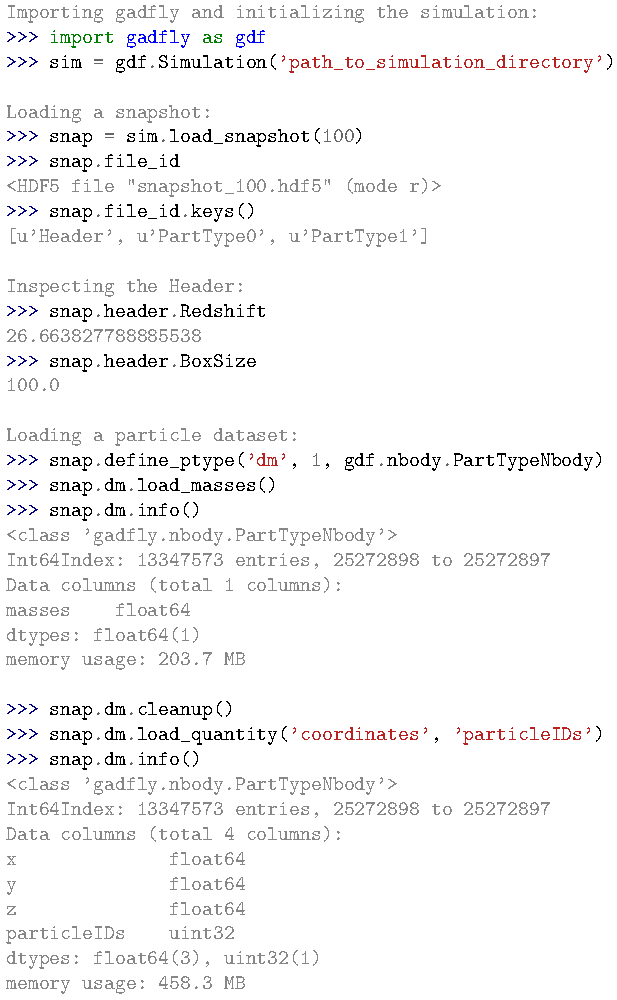
\includegraphics[width=.8\columnwidth]{figures/code_usage/code_usage}
\caption{\label{fig:usage_example}
Initializing a simulation, defining a \code{PartType} dataset, and loading data.%
}
\end{center}
\end{figure}

\section{A Framework built on pandas}
\label{sec:framework}

There are several motivations for building an analysis framework around the \code{pandas DataFrame}. 
The guiding principle underlying the design of this framework is to enable exploratory investigation.
This requires both intelligent memory management for handling out-of-core datasets, and a robust indexing system to ensure that particle properties do not become misaligned in memory.
Using  the \code{pandas DataFrame} as the primary data container rather than separate \code{numpy} arrays makes it much easier to keep different particle properties indexed correctly while still affording the flexibility to load and remove data from memory at will.
In addition, \code{pandas} itself is a thoroughly documented, open-source, BSD-licensed library providing high-performance, easy-to-use data structures and analysis tools, and has a strong community of developers working to improve it.  
More broadly, as \code{pandas} is becoming the de-facto standard for data analysis in python, doing so simplifies interoperability with the rest of the available tools.

\code{Gadfly} is designed for use with simulation data stored in the HDF5 format\footnote{\code{http://www.hdfgroup.org/HDF5}}.
While we otherwise aim to keep \code{gadfly} as general as possible, some assumptions about the storage format are necessary.
Each particle type is expected to be contained in a different HDF5 group, labeled \code{PartType0, PartType1}, etc; a \code{Header} group is also expected, containing metadata for the simulation snapshot as HDF5 attributes. 
All particles are expected to have the following fields defined: particle IDs, masses, coordinates, and velocities.  
SPH particles are additionally expected to have a smoothing length, density, and internal energy.  Additional fields not included in the original \textsc{gadget} specification, such as chemical abundances, are also supported.

Here, we provide an overview of the design and capabilities of the \code{gadfly} framework, including the \code{Simulation}, \code{Snapshot}, and \code{PartType DataFrame} objects at the core of \code{gadfly} (Section \ref{sec:hierarchy}), the usage of which is demonstrated in Figure \ref{fig:usage_example}.
Our approach to file access and intelligent memory management (Section \ref{sec:fileIO}), our handling of unit conversions (Section \ref{sec:units}) and coordinate transformations (Section \ref{sec:coords}), and the included utilities for parallel batch processing (Section \ref{sec:parallel}) are also described.


\begin{figure}
\begin{center}
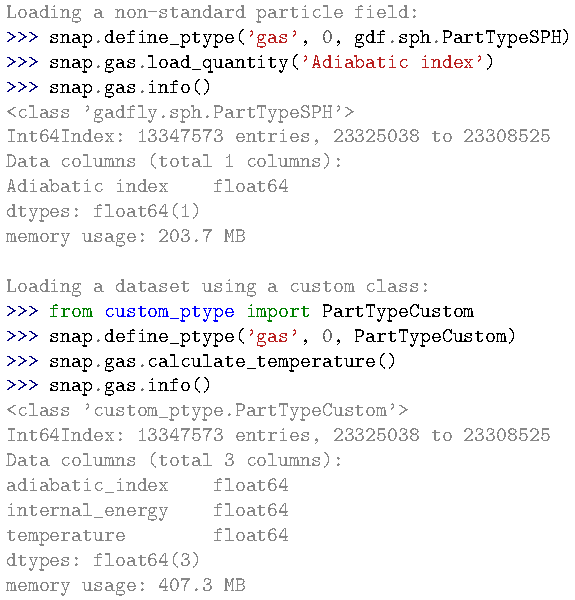
\includegraphics[width=\columnwidth]{figures/code_custom_ptypes/code_custom_ptypes}
\caption{\label{fig:custom_ptype}
Loading non-standard particle fields and defining custom PartType classes. Within \code{gadfly} this is straightforward.%
}
\end{center}
\end{figure}

\subsection{Organizational Structure}
\label{sec:hierarchy}

\subsubsection{\code{PartType} Dataframes}
\label{sec:df}
Data for each particle type (e.g., dark matter, gas, etc.) is stored in a separate \code{PartType} dataframe and indexed by particle ID number. 
Individual fields can be loaded into the dataframes and deleted at will, with coherent slicing across multiple data fields, courtesy of \code{pandas}.  
The base \code{PartType} objects, \code{PartTypeNbody} and \code{PartTypeSPH}, are standard \code{pandas} dataframes with additional functionality for loading standard \textsc{gadget} particle fields from HDF5, converting units, and performing coordinate transformations.  
As such, \code{PartType} dataframes retain all the capabilities of the \code{pandas.DataFrame} from which they inherit, and any operation that creates a new dataframe instance returns a standard \code{pandas} dataframe.  

Nonstandard particle fields (e.g., chemical abundances) can be easily loaded into \code{gadfly} as well; fields loaded in this manner simply lack automated unit conversion.
Alternatively, a custom dataframe class inheriting from \code{PartTypeNbody} or \code{PartTypeSPH} as appropriate can be defined to provide methods for loading both nonstandard particle fields and additional derived properties (e.g., temperature). An example of such a custom class---\code{PartTypeCustom.py}---is provided in the examples distributed with \code{gadfly}, and the usage of such a custom class is demonstrated in Figure \ref{fig:custom_ptype}.

\subsubsection{\code{Snapshot}}
\label{sec:snap}
Each \code{Snapshot} object represents a single HDF5 snapshot file on disk.  File access---provided by \code{h5py} \citep{h5py}---is handled via the \code{Snapshot} object, and the actual particle data, loaded as needed into the \code{PartType} dataframes described in Section \ref{sec:df}, is gathered here with each particle type contained in a separate \code{PartType} dataframe.  
The information contained in the \textsc{gadget} header is also maintained here in a \code{Header} object, along with access to the additional metadata and unit information stored in the relevant \code{Simulation} object.

\subsubsection{\code{Simulation}}
\label{sec:sim}
Metadata relevant to the simulation as a whole, such as filepaths and unit information, are stored in a \code{Simulation} object.  Initializing a \code{Simulation} object is the first step in any analysis using \code{gadfly} as this is where default values for all subsequent analysis are set, including locating all relevant snapshot files, choosing a coordinate system, and setting the field names of the default particle properties expected by \code{gadfly}.  \code{Snapshot}s are loaded via \verb|Simulation.load_snapshot()|, and the parallel batch processing functionality described in Section \ref{sec:parallel} is implemented at this level as well.

\subsection{Memory Management and File Access}
\label{sec:fileIO}
One of the primary goals of the \code{gadfly} project is to enable the analysis of large datasets on machines with limited memory.
Enabling this requires intelligent memory management, loading only the particle data of interest from the disk.
Fortunately the HDF5 protocol is well-suited to such non-contiguous file access, allowing not only individual data fields to be accessed independently, but also for  loading only select entries from the field in question.

\code{Gadfly} employs two complementary approaches to minimizing the memory footprint.
The first method requires definition of an optional refinement criterion, such as particles above a given density threshold.
The resulting `refined' index can then be used to select only the corresponding values from subsequent particle fields as they are loaded.
While this method efficiently minimizes I/O operations, it is fairly rigid, and attempting to load additional fields into a dataframe from which particles have been manually dropped will fail, as the particle indices will no longer match.  
As such, this approach is poorly suited to exploratory analysis where the proper refinement criterion may not be know \textit{a priori} and is best suited for use in scripts where the analysis to be performed is well defined.

To mitigate the indexing issues that can arise in situations where data is loaded incrementally, \code{gadfly} performs an intermediate step, first loading new fields into a \code{pandas.Series} data structure, using the particle ID numbers as an index.  This allows \code{pandas} to properly align the particle fields, dropping any particles not in the existing \code{PartType} dataframe from the newly loaded field as it is appended.
This approach, which can be used in tandem with the refinement index, affords \code{gadfly} the flexibility needed to allow incremental manual refinement of the data stored in memory. 
Additional cuts can be made as subsequent fields are loaded, resulting in the selection of a precisely targeted primary dataset from which derived  properties (e.g., temperature) may be calculated, which serves to reduce computational overhead as well.

\begin{figure}
\begin{center}
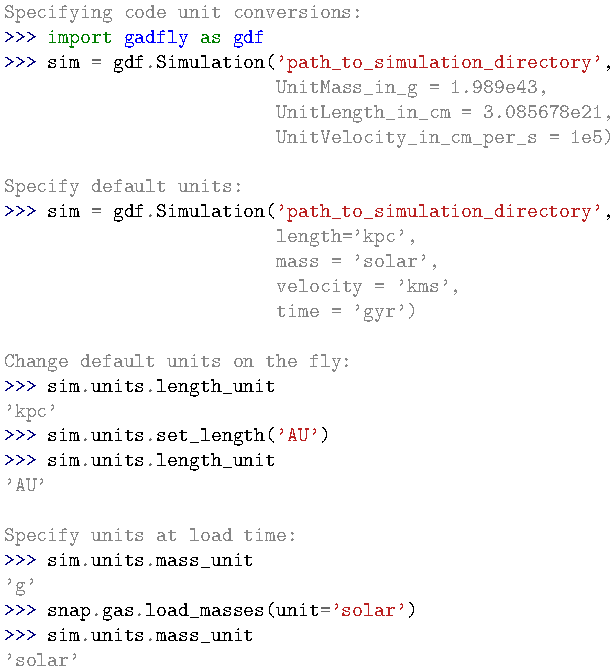
\includegraphics[width=\columnwidth]{figures/code_units/code_units}
\caption{\label{fig:units}
Unit handling in \code{gadfly}.%
}
\end{center}
\end{figure}

\subsection{Units}
\label{sec:units}
\code{Gadfly} implements a minimal unit-handling system for converting between the native code units in which \textsc{gadget} stores data and the physical units of interest to astronomers.  
However, \textsc{gadget}'s code units may be modified to suit the problem at hand, and therefore must be specified at initialization if they differ from the defaults listed in Table \ref{code_unit_defaults}.
\begin{table}
    \centering
    \caption{Default code units expected by \code{gadfly}.}
    \label{code_unit_defaults}
    \begin{tabular}{ll}
        \hline
        Unit & Conversion to \verb|cgs|\\
        \hline
        \verb|Mass| &  $1.989\times10^{43}\,$g\\ 
        \verb|Length| & $3.085678\times10^{21}\,$cm \\ 
        \verb|Velocity| & $1.0\times10^5\,$cm$\,$s$^{-1}$ \\ 
    \end{tabular} 
\end{table}
Conversion from code units to the physical units system of choice is handled at loading.
The default units for length, time, mass, etc. can be specified at initialization, along with whether to use physical or comoving coordinates (for cosmological simulations) and whether to factor the Hubble constant out of the reported units (i.e., units of Mpc vs. Mpc/$h$).
While defaults are set at startup, they can be modified at any time, either by calling \verb|units.set_length()|, which alters the default length unit for all subsequently loaded fields, or by calling a particle field's load function with the optional \code{units} keyword argument.  
Changing the units of an existing field can be done by simply reloading it; the field will remain properly indexed as described in Section \ref{sec:fileIO}. Examples of both approaches to unit conversions are shown in Figure \ref{fig:units}.

%\clearpage
\subsection{Coordinate Transformations}
\label{sec:coords}
A full suite of coordinate transformation utilities is included in \code{gadfly}, with methods for converting between Cartesian, spherical, and cylindrical coordinates, performing linear coordinate translations, and rotations about arbitrary axes.  
These methods are both directly accessible as independent library functions, and via the \code{PartType} dataframe object using the \verb|.orient_box()| functionality.

\subsection{Parallel Batch Processing}
\label{sec:parallel}
Investigating the results of a simulation often requires running an identical analysis on many snapshots in order to study how the system changes with time.  
These operations are typically completely independent, and thus amenable to parallelization---so long as the machine being used has sufficient memory.
To aid in the parallelization of such analyses, \code{gadfly} includes utilities for performing parallel batch processing jobs by making use of python's \code{multiprocessing} module. 

One issue with doing operations such as this in parallel is that they are often IO-bound.
To mitigate the issues that arise when multiple processes attempt to read large amounts of data from disk simultaneously, \code{gadfly}'s parallelization utilities are designed to load the data needed for a given analysis serially in a separate thread from the main execution. 
As the necessary data from each snapshot file is loaded, execution is passed to a pool of worker processes which can then perform the remainder of the analysis in parallel.  An example of such a parallel batch processing script is included in the examples distributed with \code{gadfly}.

\begin{figure}
\begin{center}
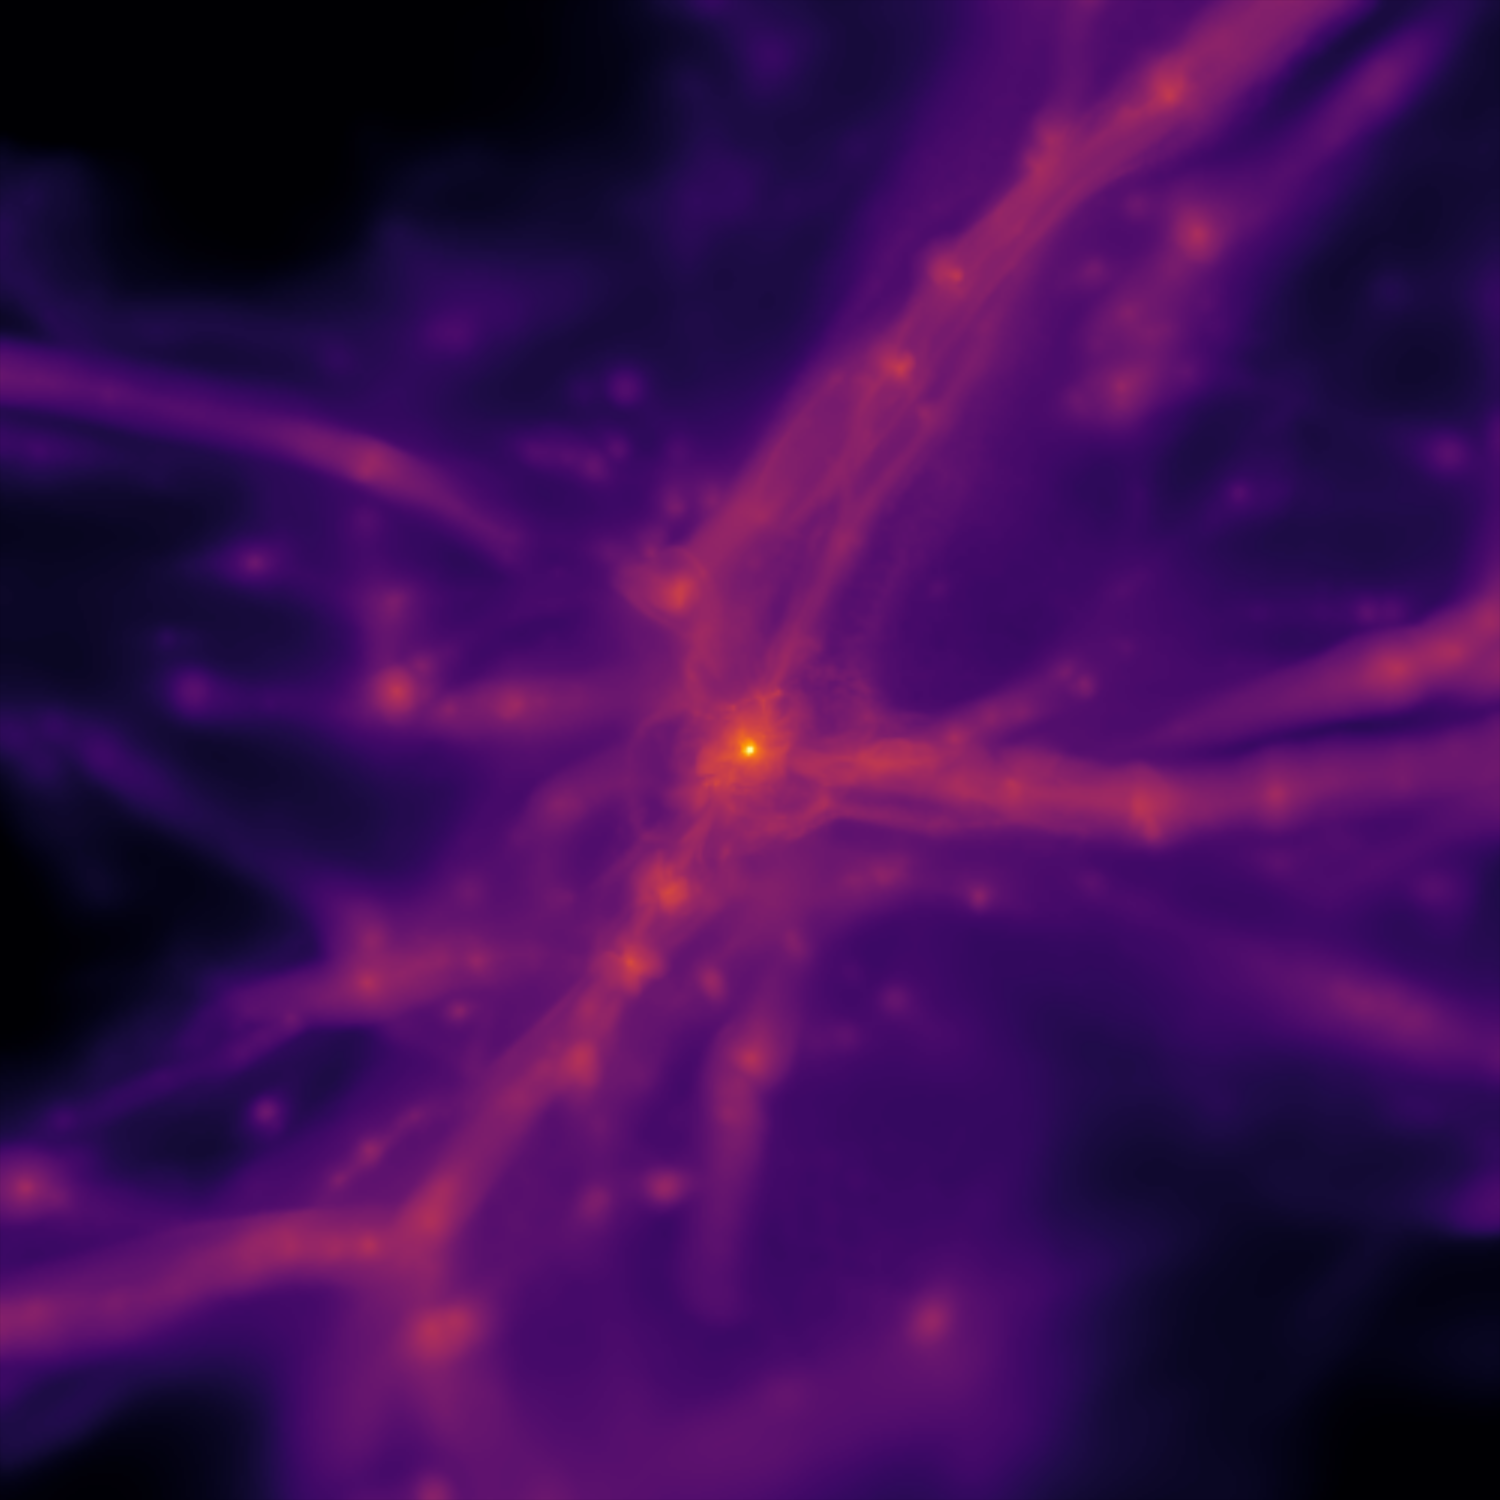
\includegraphics[width=\columnwidth]{figures/structure_halo/structure_halo}
\caption{\label{fig:vis}
Example of a visualization produced by \code{gadfly}.  This particular image shows the density distribution in a minihalo forming at $z=25$ on $1\,{\mathrm kpc}$ scales, and is from a simulation run for \citet{Hummeletal2015}.%
}
\end{center}
\end{figure}

\section{Visualization}
\label{sec:vis}
Visualization plays a major role in any analysis of simulation data, and the ability to directly visualize the spatial structure and evolution of a system is often crucial to generating insight.
While the guiding principle of the \code{gadfly} project is to avoid reinventing the wheel, instead relying on the tools developed by the broader scientific python community wherever possible, SPH particle rendering is one critical area where that broader ecosystem proves insufficient.  
To mitigate this shortcoming, \code{gadfly} includes a minimal library of visualization tools.

The particles in an SPH simulation are best thought of as fluid elements sampling the continuum properties of the gas they represent \citep{Lucy1977,GingoldMonaghan1977,Monaghan1992,Springel2010}.  They accomplish this by serving as Lagrangian tracers over which the continuum properties are interpolated using a smoothing kernel $W$. While it is possible to use alternative kernels, most modern SPH implementations (including \textsc{gadget}) utilize a cubic spline kernel \citep{Springel2014}: 
\begin{equation}
W(r,h_{\mathrm sml}) =
     \begin{cases}
       1 - 6 \left( \frac{r}{h_{\mathrm sml}} \right)^2 + 6 \left( \frac{r}{h_{\mathrm sml}} \right)^3, & 0 \leq \frac{r}{h_{\mathrm sml}} \leq \frac{1}{2}\\
       2 \left(1 - \frac{r}{h_{\mathrm sml}}\right)^3, & \frac{1}{2} < \frac{r}{h_{\mathrm sml}} \leq 1\\
       0, & \frac{r}{h} >  1,\\
     \end{cases}
\end{equation}
where $r$ is the radius and $h_{\mathrm sml}$ is the characteristic width of the kernel, otherwise known as the smoothing length.  The physical density at any point, $\rho(\mathbf{r})$, is then represented by the sum over all particles
\begin{equation}
\rho({\mathbf r}) \simeq \sum_j m_j W({\mathbf r} - {\mathbf r}_j, h_{\mathrm sml}),
\end{equation}
where $m_j$ is the mass of particle $j$, located at ${\mathbf r}_j$.
As such, creating visualizations that faithfully reproduce the actual density distribution requires performing this sum over all particles of interest; this can be quite computationally intensive depending on the number of particles involved and the desired resolution.
The SPH particle rendering algorithm included in \code{gadfly} performs this summation over two dimensions, producing a density-weighted projection. An example of such a visualization produced by \code{gadfly} is shown in Figure \ref{fig:vis}.

\code{Gadfly} includes three separate implementations of this algorithm, each of which is best suited to different conditions:
\begin{enumerate}
\item The primary implementation is derived from \citet{NavratilJohnsonBromm2007} and is written in \code{C}, parallelized using OpenMP, and wrapped in python using \code{scipy.weave}.  This method must be locally compiled, and will fail if the python interpreter cannot locate a \code{C} compiler, or if the requisite libraries are not installed.  However, it its the most powerful implementation, best suited to rendering many particles, and to machines with many processors available.
\item A second implementation makes use of \code{numba} \citep{LamPitrouSeibert2015} to perform just-in-time (JIT) compilation of pure python code using the LLVM compiler infrastructure \citep{LattnerAdve2004}.  The resulting serial routine is highly optimized, providing performance within a factor of two of the parallel method on a 16-core machine.  As such, this method is preferable on smaller machines with fewer processors, and for visualizations including fewer particles where the additional overhead associated with the parallel implementation is significant.
\item The final implementation is a pure python routine included only for situations where the other methods have unmet dependencies. This implementation is over 500 times slower than the others, and as such is suitable only to visualizing small numbers of particles, or as a last resort.
\end{enumerate}

These methods are all available as independent library functions, and can be used both with particle data in a \code{PartType} dataframe or independently from the rest of the \code{gadfly} framework, with data stored in \code{numpy} arrays.  
Future versions of \code{gadfly} will greatly simplify the visualization of data stored in a \code{PartType} dataframe through the use of a \code{.visualize()} method (see Section \ref{sec:future}).

\section{Future Development}
\label{sec:future}
The \code{gadfly} package is under active development, and in addition to incremental improvements of the existing functionality, a few significant upgrades are planned for future releases.  
First and foremost, the current \code{gadfly} units system is fairly inflexible, with limited support for additional units.  
For the next release we plan on replacing the existing units system, instead employing the far more versatile \code{astropy.units} framework \citep{Robitailleetal2013} as the backend for handling unit conversions. 
Future releases will also more seamlessly integrate \code{gadfly}'s visualization tools with the rest of the framework.  
At the moment the user is required to pass each required field to the visualization methods individually.
We intend to integrate this functionality directly into the \code{PartType} dataframe, allowing the user to simply call \code{PartType.visualize()} and be presented with a default density projection of the SPH particles currently in the dataframe, similar to the \code{.plot()} functionality of a standard \code{pandas.DataFrame}.

In the longer term, the \code{dask}\footnote{\code{http://dask.pydata.org}} project presents an intriguing option for handling very large out-of-core datasets through the use of blocked algorithms and task scheduling.
\code{Dask} manages this by mapping high-level \code{numpy}, \code{pandas}, and list operations on large datasets to many operations on smaller chunked datasets that can fit in memory.  
Future releases of \code{gadfly} may migrate the data structure on which the \code{PartType} dataframe is built from the \code{pandas.DataFrame} to \code{dask.dataframe} to take advantage of this functionality.

\section{Summary}
\label{sec:summary}
In this paper we have presented the first public release of \code{gadfly}.  We have described the framework's structure, which is designed around three core abstractions: the \code{PartType} dataframe (Section \ref{sec:df}), the \code{Snapshot} object (Section \ref{sec:snap}), and the \code{Simulation} object (Section \ref{sec:sim}).  Additional functionality includes intelligent memory management and file access (Section \ref{sec:fileIO}), basic unit handling (Section \ref{sec:units}), coordinate transformations (Section \ref{sec:coords}), utilities for parallel batch processing (Section \ref{sec:parallel}), and SPH particle visualization (Section \ref{sec:vis}).

\code{Gadfly} is fully open-source, is released under the MIT License, and can be downloaded and installed from its repository at \code{http://github.com/hummel/gadfly}.  Users can submit bug reports via GitHub, and if they know how to fix them, are welcome to submit pull requests.


\begin{appendix}
\chapter{Appendix}
\label{appendix}
Included here are the observable properties of the He100 and R175 models from
\citet{KasenWoosleyHeger2011}, including the observable flux and time visible 
(\RefFig{visibility2}) and the observable number for each feedback scenario 
(\RefFig{obsnumber2}).  These plots are to be compared to
\RefFig{visibility} and \RefFig{obsnumber} in \RefSec{JWSTobs}.  Both
cases may be detected with NIRCam beyond $z=15$ for deep exposures of
$10^6\,$s.

Also included is an extended version of \RefFig{area_obsR250} showing
the detectable number in observing campaigns totalling $10^6$, $10^7$
and $10^8\,$s for all four PISN models (\RefFig{area_obs}). Only
R250-type PISNe will be detectable above reshift 15, and R175- and
B200-type PISNe will only be detectable in observing campaigns
totalling greater than $10^7\,$s.

\begin{figure}
 \begin{center}
   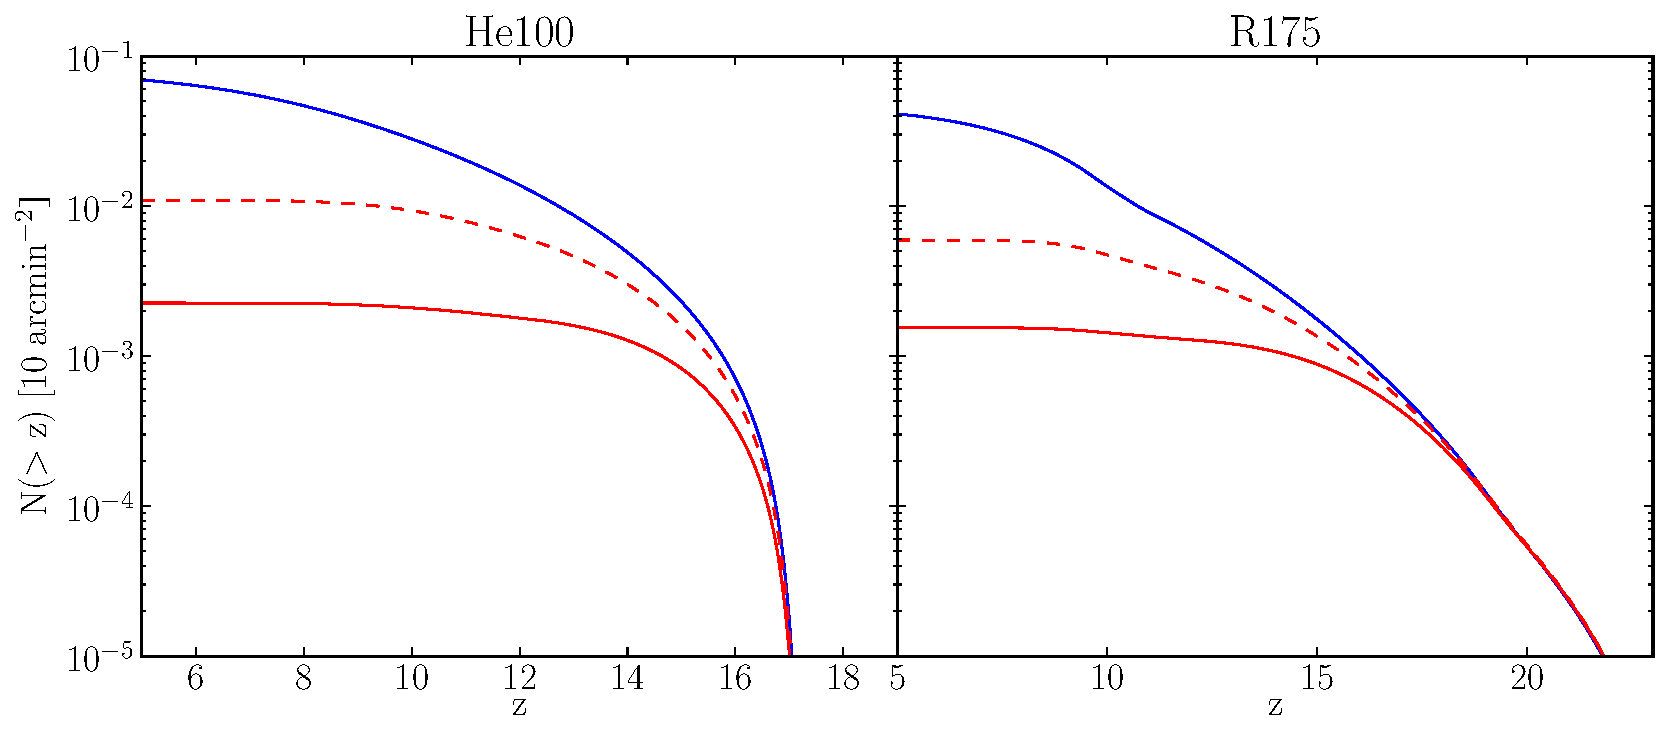
\includegraphics[width=\columnwidth]{observableNumber2}
   \caption{Upper and lower limits for the number of
     PISNe per JWST FoV above redshift $z$ with different feedback
     prescriptions. The observable numbers for a $10^6\,$s exposure
     assuming the He100 model are shown on the left; the R175 model is
     employed on the right. Solid blue lines show an upper limit
     to the observable number in the case of no feedback, solid red
     lines an estimate for the observable number in our conservative
     feedback scenario, and dashed red lines the number in the
     enhanced star formation case. Note that the x-axis is scaled
     independently in each panel.  }
   \label{obsnumber2}
 \end{center}
\end{figure} 

\begin{figure}
  \vspace*{\fill}
  \begin{center}
    \resizebox{15cm}{12cm}
              {\unitlength1cm
                \begin{picture}(15,12)
                  \put(0,6){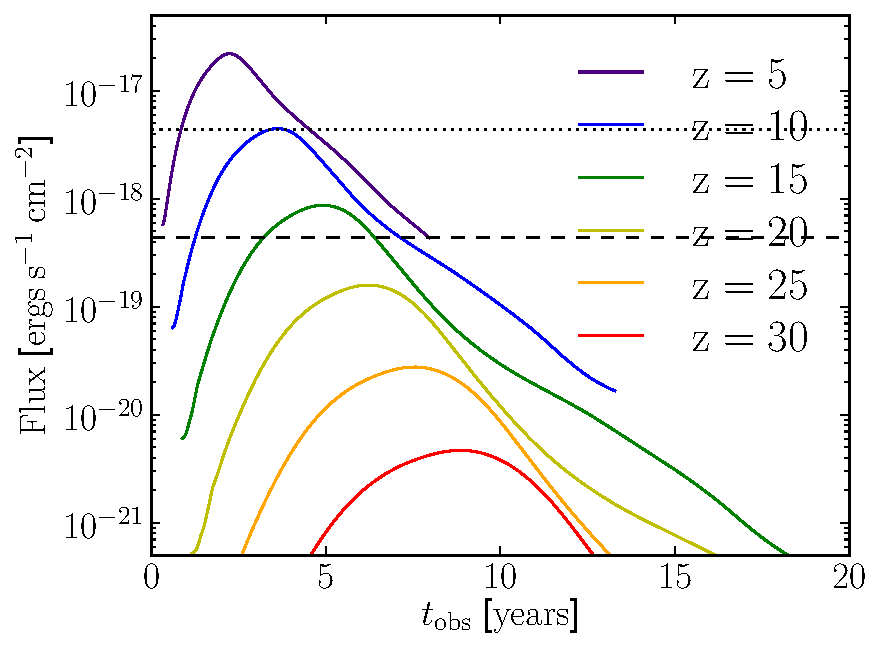
\includegraphics[width=7.5cm,height=6cm]{H100flux_F444W}}
                  \put(7.5,6){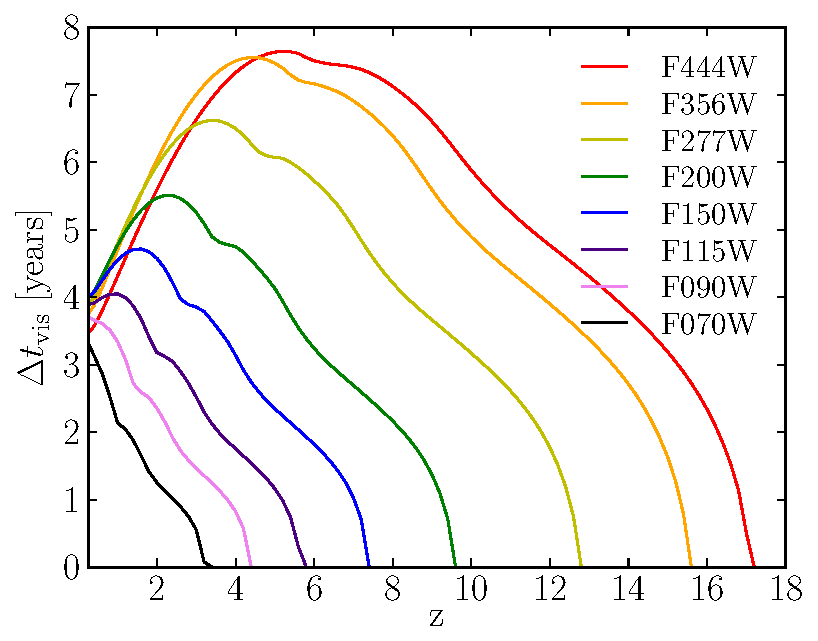
\includegraphics[width=7.5cm,height=6cm]{H100_t6}}
                  \put(0,0){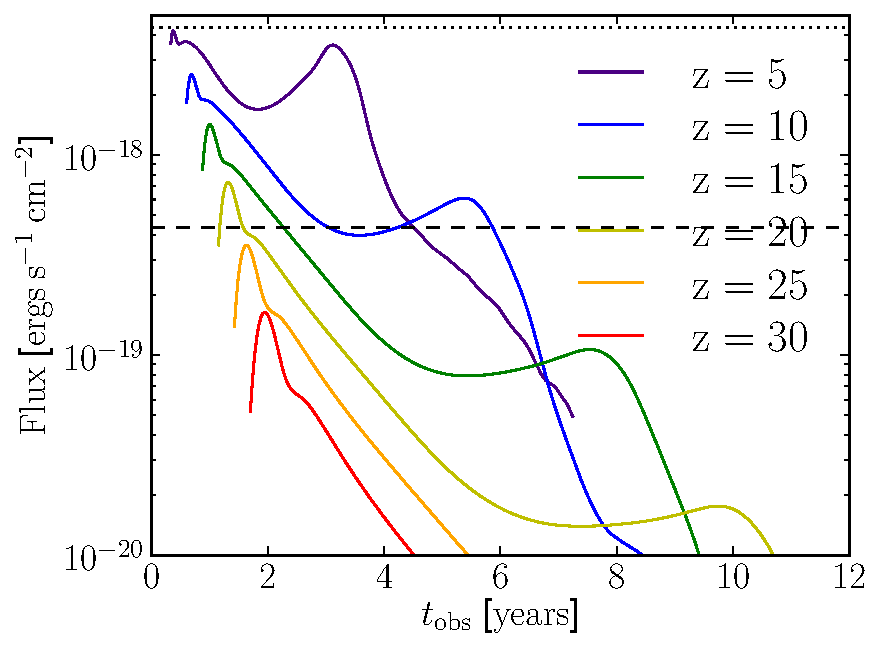
\includegraphics[width=7.5cm,height=6cm]{R175flux_F444W}}
                  \put(7.5,0){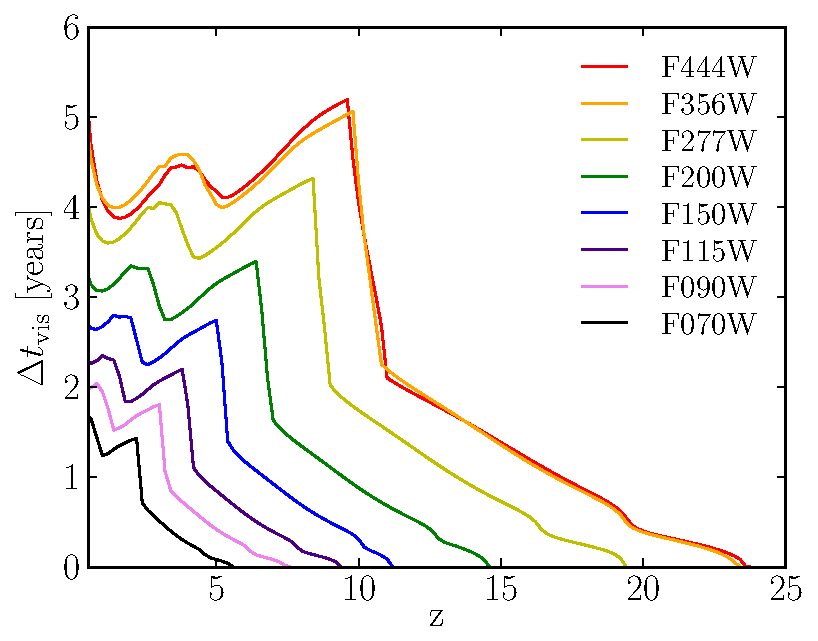
\includegraphics[width=7.5cm,height=6cm]{R175_t6}}
              \end{picture}}
              \caption{Left: Lightcurves for the
                \citet{KasenWoosleyHeger2011} He100 (top) and R175
                (bottom) models as they would be observed by JWST's
                F444W NIRCam filter at $z = 5, 10, 15, 20, 25 \:{\mathrm
                  and}\: 30$. The flux limits for a $10^6\,$s (dashed
                line) and $10^4\,$s (dotted line) exposure are shown
                for reference.  Right: The visibility time $\Delta
                t_{\mathrm vis}$ in years for He100 (top) and R175
                (bottom) as a function of redshift for each of the
                NIRcam wide filters. Note that the axes are scaled
                independently.}
              \label{visibility2}
  \end{center}
  \vspace*{\fill}
\end{figure}

\begin{figure}
  \vspace*{\fill}
  \begin{center}
    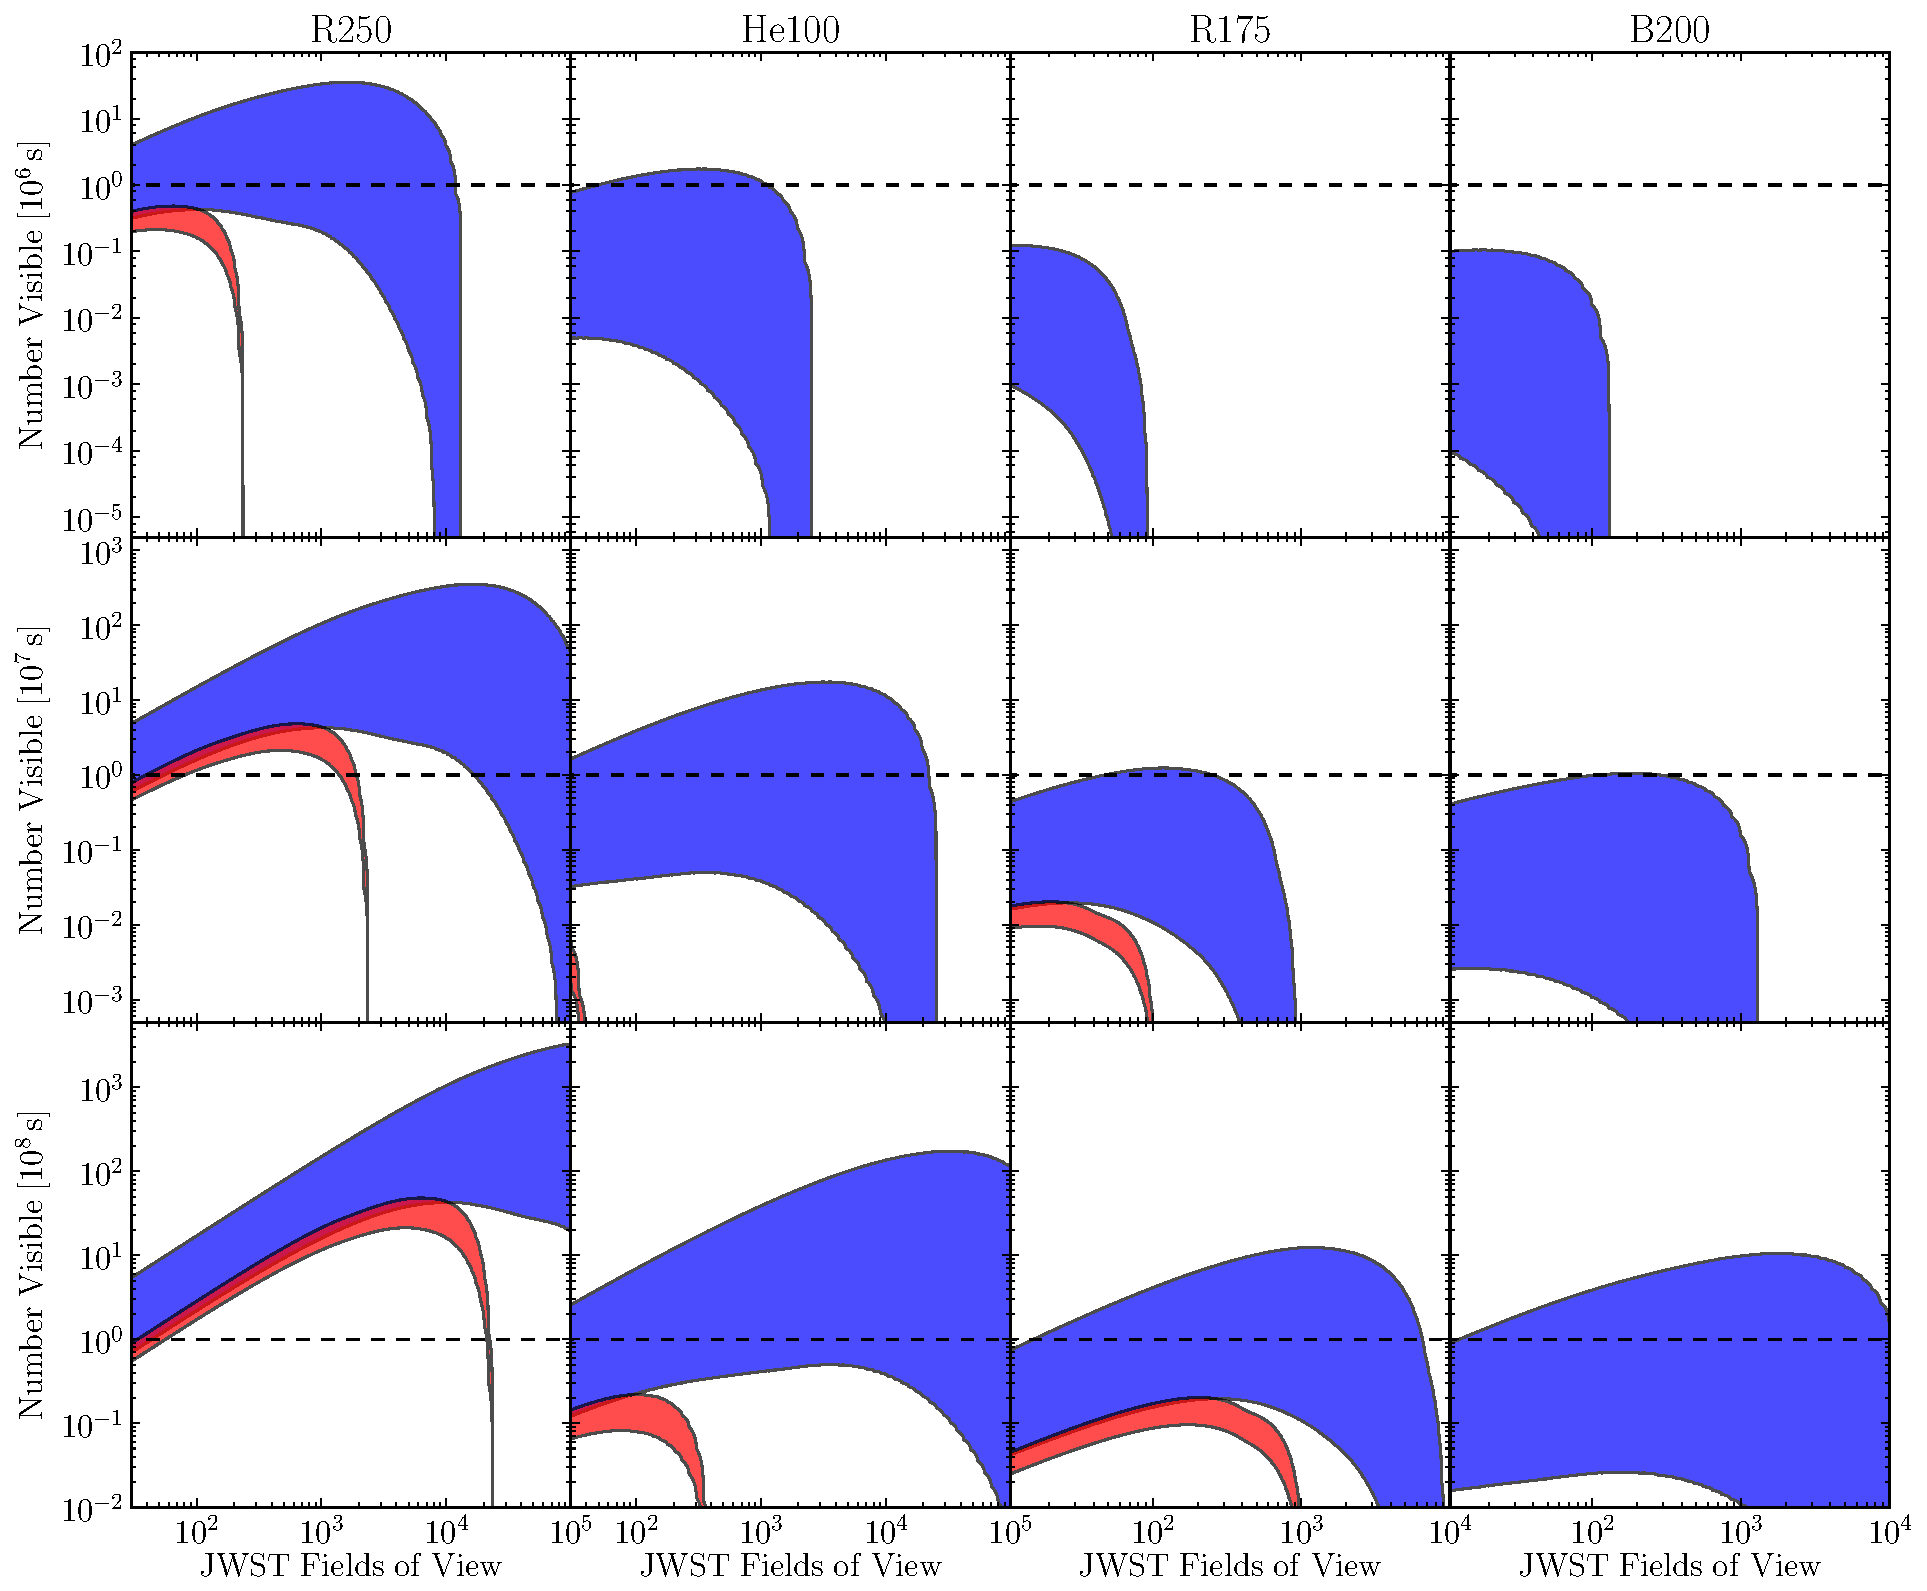
\includegraphics[width=\textwidth]{area_observability}
    \caption{The total number of PISNe observable with a
      campaign of $10^6$, $10^7$ and $10^8\,$s (from top to bottom) as
      a function of total survey area for a given PISN model.  In each
      case, the total campaign time is apportioned equally over the
      survey area to determine the exposure time for individual
      pointings.  The blue region represents all PISNe, the red only
      PISNe from $z>15$.  Upper boundaries correspond to the
      no-feedback upper limit to the PISN rate and lower boundaries to
      the conservative feedback case.  The dashed line marks one PISN
      visible. Note that not all axes are scaled the same.  }
    \label{area_obs}
  \end{center}
  \vspace*{\fill}
\end{figure} 
\end{appendix}


\backmatter

\printindex

\cleardoublepage
\phantomsection
\addcontentsline{toc}{chapter}{Bibliography}
%\chapter*{Bibliography}
\bibliography{biblio}

\end{document}
